\documentclass[journal=jctc,manuscript=article]{achemso}
\setkeys{acs}{articletitle = true}
 
%%%%%%%%%%%%%%%%%%%%%%%%%%%%%%%%%%%%%%%%%%%%%%%%%%%%%%%%%%%%%%%%%%%%%
%% Place any additional packages needed here.  Only include packages
%% which are essential, to avoid problems later.
%%%%%%%%%%%%%%%%%%%%%%%%%%%%%%%%%%%%%%%%%%%%%%%%%%%%%%%%%%%%%%%%%%%%%
\usepackage{chemformula} % Formula subscripts using \ch{}
\usepackage[T1]{fontenc} % Use modern font encodings

%%%%%%%%%%%%%%%%%%%%%%%%%%%%%%%%%%%%%%%%%%%%%%%%%%%%%%%%%%%%%%%%%%%%%
%% If issues arise when submitting your manuscript, you may want to
%% un-comment the next line.  This provides information on the
%% version of every file you have used.
%%%%%%%%%%%%%%%%%%%%%%%%%%%%%%%%%%%%%%%%%%%%%%%%%%%%%%%%%%%%%%%%%%%%%
%%\listfiles

%%%%%%%%%%%%%%%%%%%%%%%%%%%%%%%%%%%%%%%%%%%%%%%%%%%%%%%%%%%%%%%%%%%%%
%% Place any additional macros here.  Please use \newcommand* where
%% possible, and avoid layout-changing macros (which are not used
%% when typesetting).
%%%%%%%%%%%%%%%%%%%%%%%%%%%%%%%%%%%%%%%%%%%%%%%%%%%%%%%%%%%%%%%%%%%%%
% \newcommand*\mycommand[1]{\texttt{\emph{#1}}}

\usepackage{fullpage}
\usepackage{amsfonts}
\usepackage{graphicx}
\usepackage{float}
\usepackage{amsmath}
\usepackage{chemfig}
\usepackage{indentfirst}
\usepackage{longtable}
\usepackage{array}
\usepackage{cellspace}
\usepackage{palatino}
%\usepackage{breqn}
\usepackage{amssymb}
\usepackage{verbatim}
\usepackage[hidelinks,colorlinks=false,citecolor=black,linkcolor=black]{hyperref}
\usepackage{siunitx}
\usepackage{xr}
%\usepackage{bibentry}
\usepackage{verbatim}

%\DefineVerbatimEnvironment%
%	{verbatimprog}%
%	{Verbatim}%
%	{fontsize=\footnotesize}%

\newenvironment{myequation}{%
\addtocounter{equation}{-1}
\refstepcounter{defcounter}
\renewcommand\theequation{SI.\thedefcounter}
\begin{equation*}}
{\end{equation*}}

\renewcommand{\thefigure}{S\arabic{figure}}

\renewcommand{\thepage}{S\arabic{page}}

\renewcommand{\thesection}{S\arabic{section}}

\renewcommand{\thetable}{S\arabic{table}}

\makeatletter
\newcommand*{\addFileDependency}[1]{% argument=file name and extension
	\typeout{(#1)}
	\@addtofilelist{#1}
	\IfFileExists{#1}{}{\typeout{No file #1.}}
}
\makeatother

\newcommand*{\myexternaldocument}[1]{%
	\externaldocument{#1}%
	\addFileDependency{#1.tex}%
	\addFileDependency{#1.aux}%
}

\myexternaldocument{JCED_FOMMS_manuscript}

\SectionNumbersOn

% The figures are in a figures/ subdirectory.
\graphicspath{{figures/}}

%\bibliographystyle{apsrevlong}
%\bibliographystyle{apsrev}
\bibliographystyle{unsrt}
%\bibliographystyle{acs}

% italicized boldface for math (e.g. vectors)
\newcommand{\bfv}[1]{{\mbox{\boldmath{$#1$}}}}
% non-italicized boldface for math (e.g. matrices)
\newcommand{\bfm}[1]{{\bf #1}}          

%\newcommand{\bfm}[1]{{\mbox{\boldmath{$#1$}}}}
%\newcommand{\bfm}[1]{{\bf #1}}
\newcommand{\expect}[1]{\left \langle #1 \right \rangle} % <.> for denoting expectations over realizations of an experiment or thermal averages

\newcommand{\var}[1]{{\mathrm var}{(#1)}}
\newcommand{\x}{\bfv{x}}
\newcommand{\y}{\bfv{y}}
\newcommand{\f}{\bfv{f}}

\newcommand{\hatf}{\hat{f}}

\newcommand{\bTheta}{\bfm{\Theta}}
\newcommand{\btheta}{\bfm{\theta}}
\newcommand{\bhatf}{\bfm{\hat{f}}}
\newcommand{\Cov}[1] {\mathrm{cov}\left( #1 \right)}
\newcommand{\T}{\mathrm{T}}                                % T used in matrix transpose

\author{Richard A. Messerly}
\email{richard.messerly@nist.gov}
\affiliation{Thermodynamics Research Center, National Institute of Standards and Technology, Boulder, Colorado, 80305, United States}

\author{Mohammad S. Barhaghi}
\affiliation{Department of Chemical Engineering and Materials Science, Wayne State University, Detroit, Michigan 48202, United States}

\author{Jeffrey J. Potoff}
\affiliation{Department of Chemical Engineering and Materials Science, Wayne State University, Detroit, Michigan 48202, United States}

\author{Michael R. Shirts}
\affiliation{Department of Chemical and Biological Engineering, University of Colorado, Boulder, Colorado, 80309, United States}

%%%%%%%%%%%%%%%%%%%%%%%%%%%%%%%%%%%%%%%%%%%%%%%%%%%%%%%%%%%%%%%%%%%%%
%% The document title should be given as usual. Some journals require
%% a running title from the author: this should be supplied as an
%% optional argument to \title.
%%%%%%%%%%%%%%%%%%%%%%%%%%%%%%%%%%%%%%%%%%%%%%%%%%%%%%%%%%%%%%%%%%%%%
%\title{Multistate Bennett Acceptance Ratio replaces histogram reweighting for vapor-liquid coexistence calculations}
%\title{Multistate Bennett Acceptance Ratio to enable rapid force field parameterization}
%\title{Multistate Bennett Acceptance Ratio as a substitute for histogram reweighting when optimizing non-bonded parameters}
%\title{Multistate reweighting provides a better alternative to histogram reweighting for coexistance calculations}
%\title{Multistate histogram-free reweighting for vapor-liquid coexistence calculations of non-simulated force field parameters}
%\title{Estimating vapor-liquid coexistence properties with histogram-free reweighting}
%\title{Histogram-free reweighting for vapor-liquid coexistence calculations of multiple force fields}
\title{Supporting information: Histogram-free reweighting with grand canonical Monte Carlo: Post-simulation optimization of non-bonded potentials for phase equilibria}

%%%%%%%%%%%%%%%%%%%%%%%%%%%%%%%%%%%%%%%%%%%%%%%%%%%%%%%%%%%%%%%%%%%%%
%% Some journals require a list of abbreviations or keywords to be
%% supplied. These should be set up here, and will be printed after
%% the title and author information, if needed.
%%%%%%%%%%%%%%%%%%%%%%%%%%%%%%%%%%%%%%%%%%%%%%%%%%%%%%%%%%%%%%%%%%%%%
%\abbreviations{IR,NMR,UV}
%\keywords{MBAR, Monte Carlo, Grand Canonical, Vapor-liquid equilibria}

%%%%%%%%%%%%%%%%%%%%%%%%%%%%%%%%%%%%%%%%%%%%%%%%%%%%%%%%%%%%%%%%%%%%%
%% The manuscript does not need to include \maketitle, which is
%% executed automatically.
%%%%%%%%%%%%%%%%%%%%%%%%%%%%%%%%%%%%%%%%%%%%%%%%%%%%%%%%%%%%%%%%%%%%%
\begin{document}
	
\newpage
\clearpage
	
\section{Bonded parameters} \label{SI sec: Bonded parameters}

    \begin{table}[h!]
		\caption{Equilibrium (fixed) bond lengths $(r_{\rm eq})$. CH$_x$ and CH$_y$ represent CH$_3$, CH$_2$(sp$^3$), CH(sp$^3$), or C(sp$^3$) sites.} \label{tab:bonds}
		\begin{center}
			\begin{tabular}{|c|c|c|c|}
				\hline
				Bond sites & \multicolumn{3}{|c|}{$r_{\rm eq}$ (nm)} \\ \hline
				& TraPPE & MiPPE & NERD \\ \hline
				CH$_x$-CH$_y$ & 0.154 & 0.154 & 0.154 \\ 
				C(sp)-CH$_x$ & -- & 0.146 & -- \\
				CH$\equiv$CH & -- & 0.121 & -- \\ 
				C$\equiv$CH & -- & 0.121 & -- \\
				\hline
			\end{tabular}
		\end{center} 
	\end{table}

    \begin{table}[h!]
	\caption{Equilibrium bond angles $(\theta_{\rm eq})$ and force constants $(k_\theta/k_{\rm B})$, where $k_{\rm B}$ is the Boltzmann constant.} \label{tab:angles} % CH$_x$ and CH$_y$ represent CH$_3$, CH$_2$(sp$^3$), CH(sp$^3$), or C(sp$^3$) sites.
		\begin{center}
			\begin{tabular}{|c|c|c|c|c|}
				\hline
				Bending sites & \multicolumn{3}{|c|}{$\theta_{\rm eq}$ (degrees)} & $k_\theta/k_{\rm B}$ (K/rad$^2$) \\ \hline
				& TraPPE & MiPPE & NERD & \\ \hline
				CH$_x$-CH$_2$-CH$_y$ & 114.0 & 114.0 & 114.0 &  62500 \\ 
				CH$_x$-CH-CH$_y$ & 112.0 & 112.0 & 109.5 & 62500 \\
				CH$_x$-C-CH$_y$ & 109.5 & 109.5 & 109.5 & 62500 \\
				CH$_x$-CH$_2$-C(sp) & -- & 112 & -- & 62500 \\
				CH$_x$-C(sp)$\equiv$CH & -- & 180 & -- & 30800 \\
				CH$_x$-C(sp)$\equiv$C & -- & 180 & -- & 30800 \\
				\hline
			\end{tabular}
		\end{center} 
	\end{table}

    \begin{table}[h!]
		\caption{Fourier constants $(c_n/k_{\rm B})$ in units of K.} \label{tab:torsions} %CH$_x$ and CH$_y$ represent CH$_3$, CH$_2$(sp$^3$), CH(sp$^3$), or C(sp$^3$) sites.
		\begin{center}
			\begin{tabular}{|c|c|c|c|c|}
				\hline
				Torsion sites & $c_0/k_{\rm B}$ & $c_1/k_{\rm B}$ & $c_2/k_{\rm B}$ & $c_3/k_{\rm B}$ \\ \hline
				CH$_x$-CH$_2$-CH$_2$-CH$_y$ & 0.0 & 355.03 & -68.19 & 791.32 \\ 
				CH$_x$-CH$_2$-CH-CH$_y$ & -251.06 & 428.73 & -111.85 & 441.27 \\
				CH$_x$-CH$_2$-C-CH$_y$ & 0.0 & 0.0 & 0.0 & 461.29 \\
				CH$_x$-CH-CH-CH$_y$ & -251.06 & 428.73 & -111.85 & 441.27 \\
				CH$_x$-CH$_2$-CH$_2$-C(sp) & 94.88 & 162.00 & -205.40 & 980.40 \\
				CH$_x$-CH$_2$-C(sp)$\equiv$C(sp) & 0 & 0 & 0 & 0 \\
				CH$_x$-CH$_2$-C(sp)$\equiv$CH(sp) & 0 & 0 & 0 & 0 \\
				CH$_x$-C(sp)$\equiv$C(sp)-CH$_y$ & 0 & 0 & 0 & 0 \\
				\hline
			\end{tabular}
		\end{center} 
	\end{table}

% In accordance with Reference \citenum{Yiannourakou2019}, we simulate cyclohexane using the TraPPE CH$_x$-CH$_2$-CH$_2$-CH$_y$ torsional parameters instead of the TraPPE C-C-C-C six-member ring torsional parameters reported in Table 3 of Reference \citenum{Keasler2012}. This choice is made to better replicate the vapor-liquid coexistence densities reported in Reference \citenum{Keasler2012}. After investigating the dihedral distributions for cyclohexane obtained with the torsional parameters from Reference \cite{Keasler2012}, we suspect there is a sign error for at least the $c_1$ term.

\newpage
\clearpage

\section{Fixed vs. flexible bonds} \label{SI sec: Fixed vs flexible bonds}

	\begin{figure}[H]
		\centering
		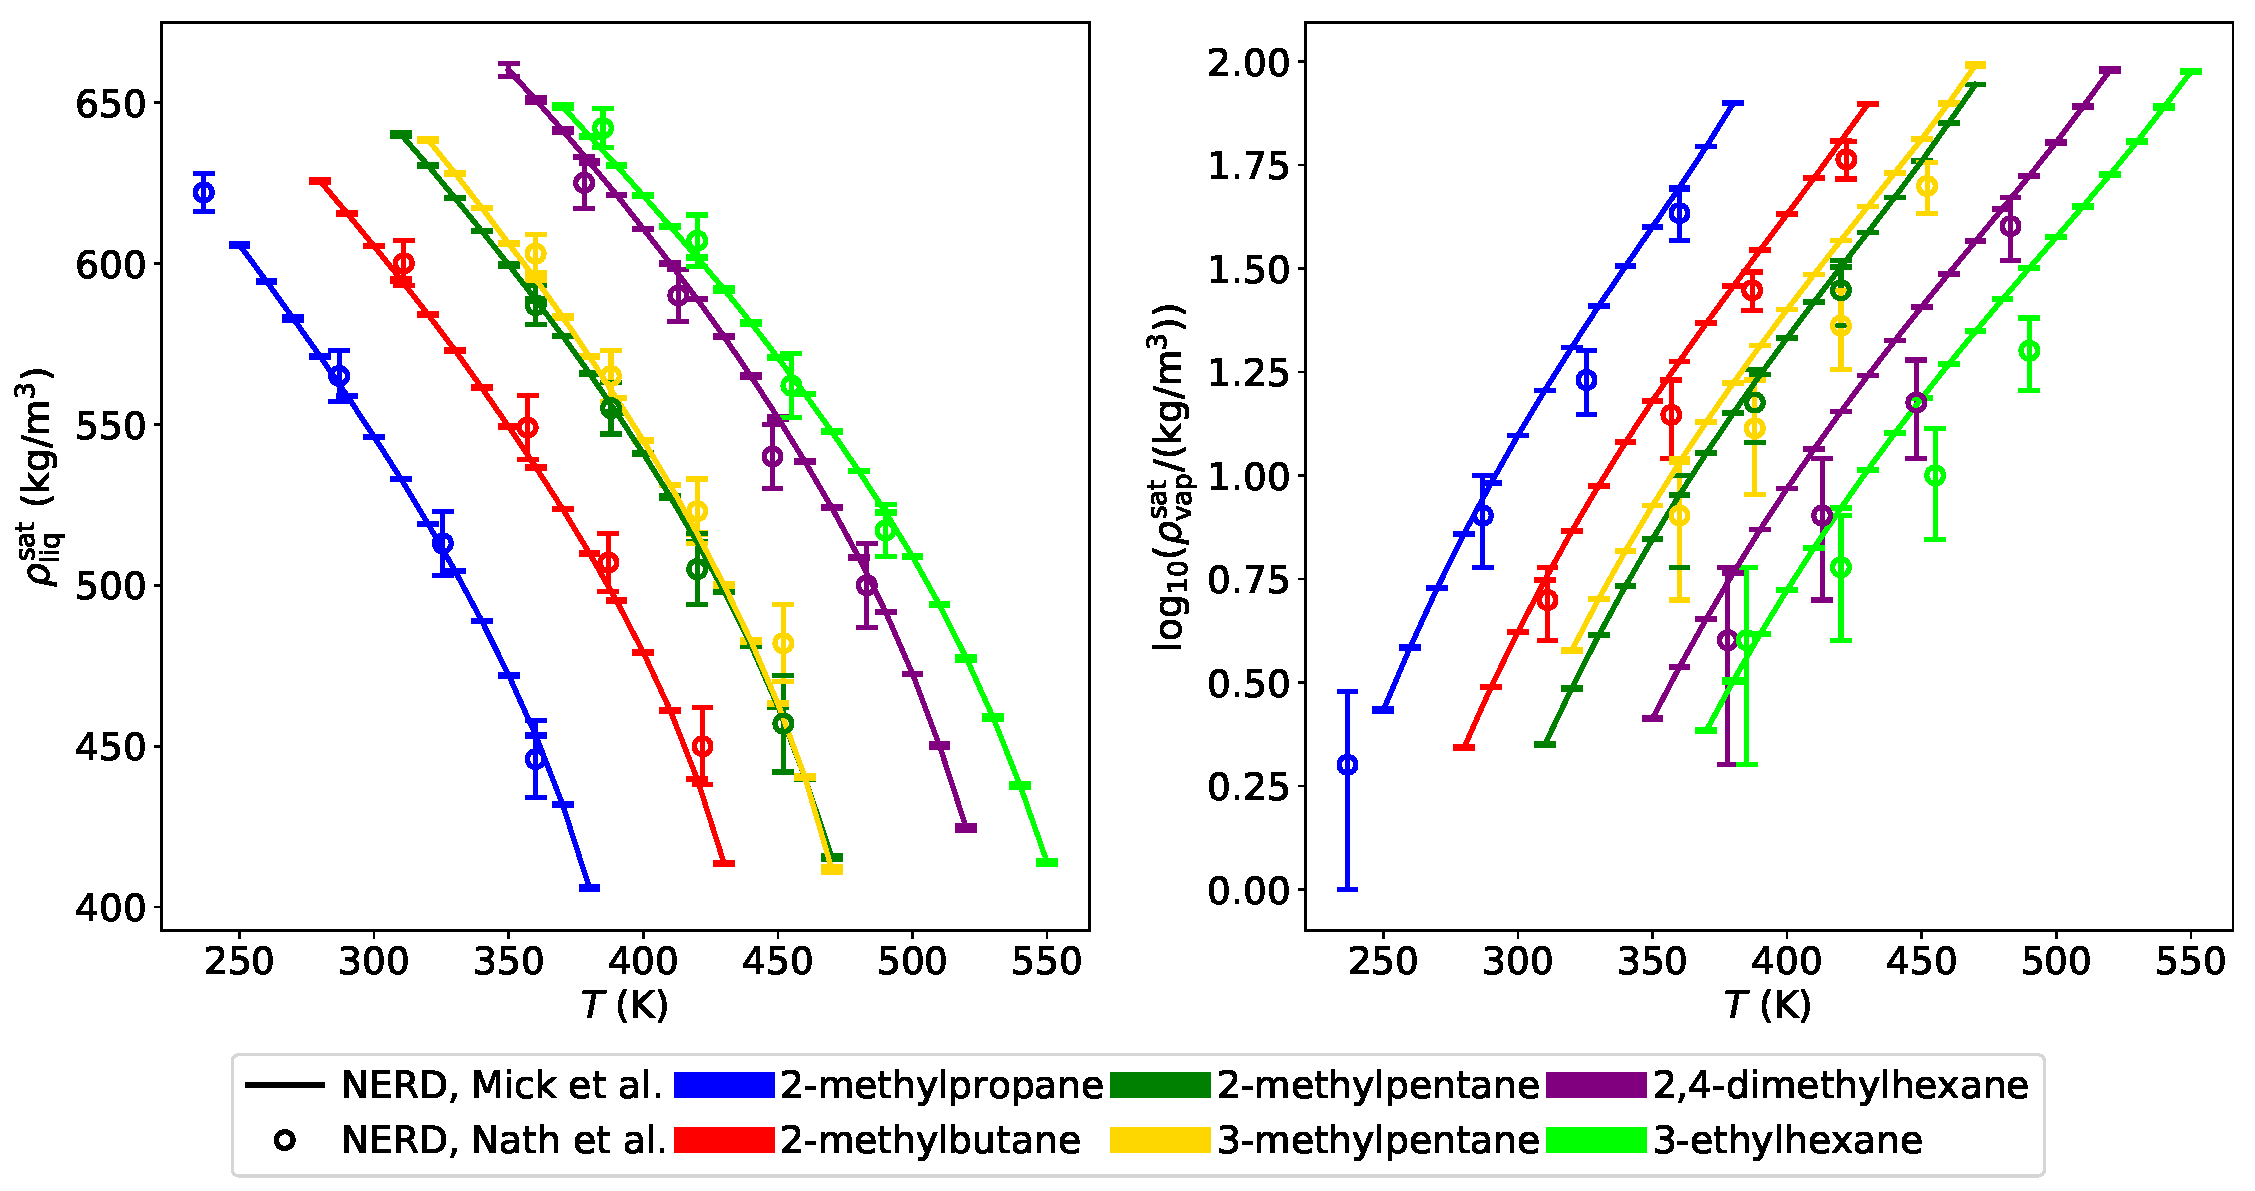
\includegraphics[width=6.4in]{NERD_fixed_flexible.pdf}
		\caption{Comparison of saturated liquid (left panel) and vapor (right panel) densities for fixed (Mick et al.) and flexible (Nath et al.) bonds. Mick et al. used GCMC-HR while Nath et al. utilized GEMC. Note that Nath et al. did not report tabulated values for vapor pressure or enthalpy of vaporization.}
		\label{SI fig: NERD_fixed_flexible}
	\end{figure}

\newpage
\clearpage

\section{CBMC acceptance rates} \label{SI sec: CBMC acceptance rates}

\begin{table}[htb!]
	\caption{Percentage acceptance of CBMC moves for cyclohexane with MiPPE force field. Averages were computed from 20 replicate simulations with $L_{\rm box}$ = 3.0 nm.}
	\begin{center}
		\begin{tabular}{|c|c|c|}
			\hline
			$T$ (K) & $\mu$ (K) & Acceptance (\%) \\ \hline
			450	&	-4370	&	68.8	\\
			500	&	-4370	&	75.1	\\
			550	&	-4370	&	39.5	\\
			500	&	-4135	&	5.50	\\
			460	&	-4025	&	2.20	\\
			410	&	-3890	&	1.11	\\
			360	&	-3790	&	0.19	\\
			\hline
		\end{tabular}
	\end{center}
\end{table}

\newpage
\clearpage

\section{Compiler and hardware} \label{SI sec: Machine hardware}

With the exception of the 20 replicates performed for MiPPE cyclohexane (3.0 and 3.5 nm box length) and TAMie cyclohexane, all simulations are run on a Linux 4.4.0-112-generic x86\_64 on an Intel(R) Xeon(R) CPU E5-2699 v4 @ 2.20GHz machine. On this machine, GOMC was erroneously compiled using the sub-optimal GNU compiler collection (GCC) instead of the preferred Intel compiler. GOMC compiled with the Intel compiler typically runs approximately twice as fast as GOMC compiled with the GCC compiler.

The 20 replicate simulations for MiPPE cyclohexane (3.0 and 3.5 nm box length) and TAMie cyclohexane utilize several different machine hardware architectures, listed in Table \ref{SI tab: Machine hardware}. GOMC was compiled with the Intel compiler on each of these machines.

\begin{table}[htb!]
	\caption{Machine hardware for 20 replicate simulations of MiPPE cyclohexane} \label{SI tab: Machine hardware}
	\begin{center}
		\begin{tabular}{|c|}
			\hline
			Intel(R) Core(TM) i7-4790K CPU @ 4.00GHz \\
			Intel(R) Core(TM) i5-3570 CPU @ 3.40GHz \\
			Intel(R) Core(TM) i5-2500K CPU @ 3.30GHz \\
			Intel(R) Xeon(R) CPU X5450 @ 3.00GHz \\
			Intel(R) Xeon(R) CPU X5355 @ 2.66GHz \\
			Intel(R) Xeon(R) CPU E5-2640 v3 @ 2.60GHz \\
			Intel(R) Core(TM)2 Quad CPU Q6600 @ 2.40GHz \\
			\hline
		\end{tabular}
	\end{center}
\end{table}

\newpage
\clearpage

\section{$\epsilon$-scaling} \label{SI sec: eps scale}

\subsection{Tabulated $\psi$ values}

\begin{table}[htb!]
	\caption{Optimal $\epsilon$-scaling parameter $(\psi)$ values and corresponding scoring function. Abbreviations correspond to those in Figure \ref{fig:epsilon_scaling}.} \label{SI tab: psi opt}
	\begin{center}
		\begin{tabular}{|c|c|c|c|}
			\hline
			Molecular name & Abbreviation & Optimal $\psi$ & Optimal score \\ \hline
			\multicolumn{4}{|c|}{Branched alkanes} \\ \hline
			2-methylpropane & 2MC$_3$ & 1.0015 & 0.3883 \\
			2-methylbutane & 2MC$_4$ & 1.0025 & 0.4281 \\
			2-methylpentane & 2MC$_5$ & 1.0020 & 0.4770 \\
			3-methylpentane & 3MC$_5$ & 1.0103 & 0.4050 \\
			2,2-dimethylpropane & 22DMC$_3$ & 1.0035 & 0.5132 \\
			2,2-dimethylbutane & 22DMC$_4$ & 0.9985 & 0.5445 \\
			2,3-dimethylbutane & 23DMC$_4$ & 1.0000 & 0.4724 \\
			2,2,4-trimethylpentane & 234TMC$_5$ & 1.0005 & 0.4367 \\ \hline	
			\multicolumn{4}{|c|}{Alkynes} \\ \hline
			1-ethyne & C$_2$ & 1.0005 & 0.2931 \\
			1-propyne & C$_3$ & 0.9965 & 0.3307 \\
			1-butyne & 1C$_4$ & 1.0063 & 1.143 \\
			2-butyne & 2C$_4$ & 1.0031 & 0.3191 \\
			1-pentyne & 1C$_5$ & 1.0087 & 1.8505 \\
			2-pentyne & 2C$_5$ & 1.0186 & 1.3801 \\
			1-hexyne & 1C$_6$ & 1.0063 & 1.908 \\
			2-hexyne & 2C$_6$ & 1.0228 & 1.0594 \\
			1-heptyne & 1C$_7$ & 1.0066 & 0.8415 \\
			1-octyne & 1C$_8$ & 1.0034 & 0.9777 \\
			1-nonyne & 1C$_9$ & 1.0000 & 0.9128 \\
			\hline
		\end{tabular}
	\end{center}
\end{table}

\newpage
\clearpage

\subsection{Tabulated phase equilibria for optimal $\psi$}

\subsubsection{Branched alkanes}

\begin{table}[htb!]
	\caption{GCMC-MBAR results for 2-methylpropane with the iMiPPE force field (optimal $\psi$ value from Table \ref{SI tab: psi opt}). Subscripts correspond to the 95\% confidence interval computed with bootstrap re-sampling.}
	\begin{center}
		\begin{tabular}{|c|c|c|c|c|c|}
			\hline
			$T^{\rm sat}$ (K) & $\rho_{\rm liq}^{\rm sat}$ (kg/m$^3$) & $\rho_{\rm vap}^{\rm sat}$ (kg/m$^3$) & $P_{\rm vap}^{\rm sat}$ (MPa) & $\Delta H_{\rm v}$ (kJ/mol) & $Z_{\rm vap}^{\rm sat}$ \\ \hline
			390 & $390.5_{4.5}$ & $85.7_{2.5}$ & $2.718_{0.030}$ & $9.90_{0.20}$ & $0.569_{0.011}$ \\
			380 & $418.0_{2.3}$ & $65.5_{2.0}$ & $2.272_{0.017}$ & $11.81_{0.14}$ & $0.639_{0.016}$ \\
			370 & $440.86_{0.43}$ & $51.3_{1.3}$ & $1.8856_{0.0088}$ & $13.31_{0.11}$ & $0.695_{0.015}$ \\
			360 & $460.16_{0.83}$ & $40.72_{0.64}$ & $1.5515_{0.0048}$ & $14.524_{0.080}$ & $0.740_{0.011}$ \\
			350 & $477.25_{0.86}$ & $32.43_{0.28}$ & $1.2638_{0.0038}$ & $15.559_{0.056}$ & $0.78_{0.01}$ \\
			340 & $492.86_{0.74}$ & $25.78_{0.16}$ & $1.0177_{0.0034}$ & $16.473_{0.048}$ & $0.81_{0.01}$ \\
			330 & $507.34_{0.80}$ & $20.38_{0.14}$ & $0.8090_{0.0033}$ & $17.292_{0.053}$ & $0.84_{0.01}$ \\
			320 & $521.13_{0.61}$ & $15.97_{0.11}$ & $0.6336_{0.0034}$ & $18.042_{0.053}$ & $0.87_{0.01}$ \\
			310 & $534.54_{0.29}$ & $12.374_{0.074}$ & $0.4881_{0.0036}$ & $18.745_{0.042}$ & $0.89_{0.01}$ \\
			300 & $547.12_{0.22}$ & $9.452_{0.060}$ & $0.3690_{0.0035}$ & $19.389_{0.035}$ & $0.910_{0.010}$ \\
			290 & $558.97_{0.19}$ & $7.101_{0.076}$ & $0.2732_{0.0032}$ & $19.980_{0.039}$ & $0.927_{0.012}$ \\
			280 & $570.80_{0.34}$ & $5.230_{0.094}$ & $0.1975_{0.0027}$ & $20.552_{0.048}$ & $0.943_{0.019}$ \\
			270 & $582.96_{0.45}$ & $3.76_{0.10}$ & $0.1389_{0.0025}$ & $21.122_{0.071}$ & $0.956_{0.034}$ \\
			260 & $593.85_{0.25}$ & $2.63_{0.10}$ & $0.0946_{0.0027}$ & $21.62_{0.12}$ & $0.966_{0.060}$ \\
			250 & $603.32_{0.94}$ & $1.787_{0.089}$ & $0.0623_{0.0034}$ & $22.06_{0.24}$ & $0.97_{0.10}$ \\
			\hline
		\end{tabular}
	\end{center}
\end{table}

\begin{table}[htb!]
	\caption{GCMC-MBAR results for 2-methylbutane with the iMiPPE force field (optimal $\psi$ value from Table \ref{SI tab: psi opt}). Subscripts correspond to the 95\% confidence interval computed with bootstrap re-sampling.}
	\begin{center}
		\begin{tabular}{|c|c|c|c|c|c|}
			\hline
			$T^{\rm sat}$ (K) & $\rho_{\rm liq}^{\rm sat}$ (kg/m$^3$) & $\rho_{\rm vap}^{\rm sat}$ (kg/m$^3$) & $P_{\rm vap}^{\rm sat}$ (MPa) & $\Delta H_{\rm v}$ (kJ/mol) & $Z_{\rm vap}^{\rm sat}$ \\ \hline
			440 & $403.0_{2.4}$ & $84.5_{1.4}$ & $2.490_{0.015}$ & $11.80_{0.11}$ & $0.58_{0.01}$ \\
			430 & $429.5_{1.4}$ & $67.3_{1.1}$ & $2.1160_{0.0099}$ & $13.658_{0.094}$ & $0.63_{0.01}$ \\
			420 & $451.56_{0.83}$ & $53.86_{0.75}$ & $1.7868_{0.0058}$ & $15.259_{0.071}$ & $0.69_{0.01}$ \\
			410 & $470.40_{0.84}$ & $43.55_{0.44}$ & $1.4985_{0.0031}$ & $16.608_{0.052}$ & $0.73_{0.01}$ \\
			400 & $487.2_{1.1}$ & $35.38_{0.25}$ & $1.2466_{0.0017}$ & $17.769_{0.044}$ & $0.76_{0.01}$ \\
			390 & $502.5_{1.3}$ & $28.74_{0.17}$ & $1.0277_{0.0016}$ & $18.796_{0.044}$ & $0.80_{0.01}$ \\
			380 & $516.7_{1.4}$ & $23.25_{0.13}$ & $0.8385_{0.0025}$ & $19.723_{0.041}$ & $0.82_{0.01}$ \\
			370 & $530.1_{1.2}$ & $18.699_{0.091}$ & $0.6765_{0.0033}$ & $20.574_{0.033}$ & $0.85_{0.01}$ \\
			360 & $542.77_{0.83}$ & $14.917_{0.061}$ & $0.5388_{0.0038}$ & $21.360_{0.027}$ & $0.87_{0.01}$ \\
			350 & $554.94_{0.49}$ & $11.782_{0.058}$ & $0.4234_{0.0039}$ & $22.094_{0.027}$ & $0.89_{0.01}$ \\
			340 & $566.86_{0.43}$ & $9.196_{0.079}$ & $0.3274_{0.0037}$ & $22.793_{0.033}$ & $0.91_{0.01}$ \\
			330 & $578.69_{0.60}$ & $7.08_{0.10}$ & $0.2489_{0.0032}$ & $23.467_{0.052}$ & $0.925_{0.011}$ \\
			320 & $589.78_{0.55}$ & $5.36_{0.12}$ & $0.1856_{0.0027}$ & $24.087_{0.073}$ & $0.939_{0.019}$ \\
			310 & $599.68_{0.39}$ & $3.99_{0.12}$ & $0.1354_{0.0024}$ & $24.634_{0.10}$ & $0.951_{0.031}$ \\
			300 & $609.37_{0.41}$ & $2.90_{0.11}$ & $0.0965_{0.0025}$ & $25.16_{0.14}$ & $0.961_{0.050}$ \\
			290 & $619.67_{0.47}$ & $2.065_{0.092}$ & $0.0670_{0.0030}$ & $25.71_{0.20}$ & $0.971_{0.076}$ \\
			\hline
		\end{tabular}
	\end{center}
\end{table}

\begin{table}[htb!]
	\caption{GCMC-MBAR results for 2-methylpentane with the iMiPPE force field (optimal $\psi$ value from Table \ref{SI tab: psi opt}). Subscripts correspond to the 95\% confidence interval computed with bootstrap re-sampling.}
	\begin{center}
		\begin{tabular}{|c|c|c|c|c|c|}
			\hline
			$T^{\rm sat}$ (K) & $\rho_{\rm liq}^{\rm sat}$ (kg/m$^3$) & $\rho_{\rm vap}^{\rm sat}$ (kg/m$^3$) & $P_{\rm vap}^{\rm sat}$ (MPa) & $\Delta H_{\rm v}$ (kJ/mol) & $Z_{\rm vap}^{\rm sat}$ \\ \hline
			470 & $424.43_{0.72}$ & $75.06_{0.98}$ & $2.0415_{0.0063}$ & $14.355_{0.063}$ & $0.60_{0.01}$ \\
			460 & $446.63_{0.44}$ & $59.92_{0.85}$ & $1.7383_{0.0032}$ & $16.259_{0.079}$ & $0.65_{0.01}$ \\
			450 & $466.02_{0.34}$ & $48.40_{0.58}$ & $1.4722_{0.0024}$ & $17.883_{0.082}$ & $0.70_{0.01}$ \\
			440 & $483.12_{0.37}$ & $39.46_{0.30}$ & $1.2388_{0.0030}$ & $19.257_{0.075}$ & $0.74_{0.01}$ \\
			430 & $498.62_{0.46}$ & $32.30_{0.13}$ & $1.0347_{0.0032}$ & $20.456_{0.064}$ & $0.77_{0.01}$ \\
			420 & $513.07_{0.46}$ & $26.404_{0.097}$ & $0.8567_{0.0028}$ & $21.538_{0.049}$ & $0.80_{0.01}$ \\
			410 & $526.79_{0.34}$ & $21.50_{0.12}$ & $0.7026_{0.0021}$ & $22.536_{0.031}$ & $0.83_{0.01}$ \\
			400 & $539.84_{0.33}$ & $17.39_{0.13}$ & $0.5701_{0.0016}$ & $23.462_{0.027}$ & $0.85_{0.01}$ \\
			390 & $552.17_{0.47}$ & $13.96_{0.12}$ & $0.4573_{0.0015}$ & $24.320_{0.043}$ & $0.87_{0.01}$ \\
			380 & $563.75_{0.44}$ & $11.10_{0.10}$ & $0.3622_{0.0018}$ & $25.113_{0.052}$ & $0.890_{0.011}$ \\
			370 & $574.77_{0.27}$ & $8.738_{0.085}$ & $0.2829_{0.0022}$ & $25.853_{0.051}$ & $0.907_{0.015}$ \\
			360 & $585.55_{0.30}$ & $6.794_{0.076}$ & $0.2177_{0.0027}$ & $26.562_{0.058}$ & $0.922_{0.021}$ \\
			350 & $596.34_{0.30}$ & $5.208_{0.079}$ & $0.1647_{0.0031}$ & $27.257_{0.083}$ & $0.936_{0.030}$ \\
			340 & $606.99_{0.31}$ & $3.928_{0.084}$ & $0.1222_{0.0035}$ & $27.93_{0.12}$ & $0.948_{0.045}$ \\
			330 & $617.01_{0.30}$ & $2.909_{0.083}$ & $0.0888_{0.0039}$ & $28.55_{0.18}$ & $0.959_{0.067}$ \\
			320 & $626.41_{0.21}$ & $2.111_{0.076}$ & $0.0631_{0.0043}$ & $29.13_{0.26}$ & $0.968_{0.099}$ \\
			\hline
		\end{tabular}
	\end{center}
\end{table}

\begin{table}[htb!]
	\caption{GCMC-MBAR results for 3-methylpentane with the iMiPPE force field (optimal $\psi$ value from Table \ref{SI tab: psi opt}). Subscripts correspond to the 95\% confidence interval computed with bootstrap re-sampling.}
	\begin{center}
		\begin{tabular}{|c|c|c|c|c|c|}
			\hline
			$T^{\rm sat}$ (K) & $\rho_{\rm liq}^{\rm sat}$ (kg/m$^3$) & $\rho_{\rm vap}^{\rm sat}$ (kg/m$^3$) & $P_{\rm vap}^{\rm sat}$ (MPa) & $\Delta H_{\rm v}$ (kJ/mol) & $Z_{\rm vap}^{\rm sat}$ \\ \hline
			480 & $428.2_{1.5}$ & $75_{12}$ & $2.171_{0.060}$ & $14.81_{0.93}$ & $0.625_{0.090}$ \\
			470 & $449.9_{1.6}$ & $61.1_{8.5}$ & $1.863_{0.021}$ & $16.56_{0.84}$ & $0.672_{0.089}$ \\
			460 & $468.1_{1.3}$ & $50.3_{4.0}$ & $1.5910_{0.0071}$ & $18.01_{0.53}$ & $0.712_{0.060}$ \\
			450 & $484.5_{1.2}$ & $41.6_{1.1}$ & $1.350_{0.014}$ & $19.28_{0.23}$ & $0.747_{0.027}$ \\
			440 & $500.3_{1.1}$ & $34.45_{0.21}$ & $1.137_{0.015}$ & $20.464_{0.074}$ & $0.78_{0.01}$ \\
			430 & $515.5_{1.0}$ & $28.41_{0.46}$ & $0.950_{0.013}$ & $21.563_{0.068}$ & $0.81_{0.01}$ \\
			420 & $529.38_{0.62}$ & $23.34_{0.40}$ & $0.786_{0.010}$ & $22.556_{0.054}$ & $0.83_{0.01}$ \\
			410 & $541.89_{0.69}$ & $19.07_{0.30}$ & $0.6449_{0.0079}$ & $23.443_{0.043}$ & $0.85_{0.01}$ \\
			400 & $553.62_{0.90}$ & $15.49_{0.24}$ & $0.5233_{0.0062}$ & $24.264_{0.049}$ & $0.88_{0.01}$ \\
			390 & $565.07_{0.63}$ & $12.48_{0.20}$ & $0.4198_{0.0048}$ & $25.051_{0.039}$ & $0.89_{0.01}$ \\
			380 & $575.97_{0.45}$ & $9.95_{0.17}$ & $0.3326_{0.0039}$ & $25.789_{0.043}$ & $0.912_{0.014}$ \\
			370 & $586_{95}$ & $7.8_{1.6}$ & $0.260_{0.066}$ & $26.5_{4.1}$ & $0.93_{0.18}$ \\
			360 & $597.06_{0.27}$ & $6.10_{0.13}$ & $0.2001_{0.0035}$ & $27.178_{0.094}$ & $0.945_{0.029}$ \\
			350 & $607.29_{0.23}$ & $4.67_{0.12}$ & $0.1514_{0.0039}$ & $27.83_{0.14}$ & $0.959_{0.043}$ \\
			\hline
		\end{tabular}
	\end{center}
\end{table}

\begin{table}[htb!]
	\caption{GCMC-MBAR results for 2,2-dimethylpropane with the iMiPPE force field (optimal $\psi$ value from Table \ref{SI tab: psi opt}). Subscripts correspond to the 95\% confidence interval computed with bootstrap re-sampling.}
	\begin{center}
		\begin{tabular}{|c|c|c|c|c|c|}
			\hline
			$T^{\rm sat}$ (K) & $\rho_{\rm liq}^{\rm sat}$ (kg/m$^3$) & $\rho_{\rm vap}^{\rm sat}$ (kg/m$^3$) & $P_{\rm vap}^{\rm sat}$ (MPa) & $\Delta H_{\rm v}$ (kJ/mol) & $Z_{\rm vap}^{\rm sat}$ \\ \hline
			410 & $413.2_{2.6}$ & $75.9_{2.6}$ & $2.173_{0.029}$ & $11.65_{0.11}$ & $0.606_{0.013}$ \\
			400 & $437.1_{2.3}$ & $59.3_{1.8}$ & $1.831_{0.018}$ & $13.410_{0.083}$ & $0.669_{0.014}$ \\
			390 & $457.4_{1.5}$ & $47.4_{1.1}$ & $1.532_{0.010}$ & $14.814_{0.051}$ & $0.719_{0.013}$ \\
			380 & $474.6_{1.1}$ & $38.29_{0.72}$ & $1.2725_{0.0056}$ & $15.944_{0.045}$ & $0.759_{0.011}$ \\
			370 & $489.78_{0.98}$ & $31.00_{0.48}$ & $1.0468_{0.0035}$ & $16.909_{0.045}$ & $0.792_{0.011}$ \\
			360 & $504.12_{0.89}$ & $25.02_{0.33}$ & $0.8520_{0.0036}$ & $17.785_{0.044}$ & $0.821_{0.012}$ \\
			350 & $518.05_{0.86}$ & $20.05_{0.21}$ & $0.6853_{0.0043}$ & $18.604_{0.046}$ & $0.847_{0.011}$ \\
			340 & $531.32_{0.93}$ & $15.93_{0.18}$ & $0.5437_{0.0045}$ & $19.363_{0.057}$ & $0.871_{0.011}$ \\
			330 & $543.65_{0.96}$ & $12.52_{0.23}$ & $0.4252_{0.0041}$ & $20.056_{0.078}$ & $0.893_{0.016}$ \\
			320 & $555.0_{1.0}$ & $9.71_{0.28}$ & $0.3271_{0.0037}$ & $20.68_{0.11}$ & $0.913_{0.029}$ \\
			310 & $565.5_{1.4}$ & $7.43_{0.32}$ & $0.2473_{0.0044}$ & $21.25_{0.18}$ & $0.931_{0.052}$ \\
			300 & $576.4_{1.8}$ & $5.60_{0.33}$ & $0.1832_{0.0061}$ & $21.82_{0.28}$ & $0.947_{0.087}$ \\
			290 & $588.4_{1.3}$ & $4.13_{0.32}$ & $0.1327_{0.0084}$ & $22.41_{0.38}$ & $0.96_{0.14}$ \\
			280 & $600.2_{1.1}$ & $2.98_{0.29}$ & $0.093_{0.011}$ & $22.98_{0.55}$ & $0.97_{0.22}$ \\
			\hline
		\end{tabular}
	\end{center}
\end{table}

\begin{table}[htb!]
	\caption{GCMC-MBAR results for 2,2-dimethylbutane with the iMiPPE force field (optimal $\psi$ value from Table \ref{SI tab: psi opt}). Subscripts correspond to the 95\% confidence interval computed with bootstrap re-sampling.}
	\begin{center}
		\begin{tabular}{|c|c|c|c|c|c|}
			\hline
			$T^{\rm sat}$ (K) & $\rho_{\rm liq}^{\rm sat}$ (kg/m$^3$) & $\rho_{\rm vap}^{\rm sat}$ (kg/m$^3$) & $P_{\rm vap}^{\rm sat}$ (MPa) & $\Delta H_{\rm v}$ (kJ/mol) & $Z_{\rm vap}^{\rm sat}$ \\ \hline
			470 & $410.4_{5.2}$ & $86.7_{8.5}$ & $2.34_{0.11}$ & $12.61_{0.20}$ & $0.595_{0.027}$ \\
			460 & $436.5_{4.9}$ & $70.3_{8.7}$ & $2.014_{0.071}$ & $14.48_{0.34}$ & $0.645_{0.049}$ \\
			450 & $457.9_{3.1}$ & $57.7_{7.2}$ & $1.724_{0.036}$ & $16.04_{0.45}$ & $0.689_{0.061}$ \\
			440 & $476.4_{1.5}$ & $47.7_{4.6}$ & $1.467_{0.011}$ & $17.37_{0.41}$ & $0.725_{0.057}$ \\
			430 & $493.01_{0.95}$ & $39.4_{2.1}$ & $1.2386_{0.0045}$ & $18.53_{0.25}$ & $0.757_{0.039}$ \\
			420 & $508.03_{0.71}$ & $32.56_{0.58}$ & $1.0375_{0.0094}$ & $19.573_{0.098}$ & $0.786_{0.020}$ \\
			410 & $521.74_{0.38}$ & $26.79_{0.14}$ & $0.862_{0.010}$ & $20.513_{0.035}$ & $0.81_{0.01}$ \\
			400 & $534.75_{0.29}$ & $21.94_{0.16}$ & $0.7088_{0.0094}$ & $21.383_{0.026}$ & $0.84_{0.01}$ \\
			390 & $547.49_{0.34}$ & $17.86_{0.11}$ & $0.5771_{0.0086}$ & $22.210_{0.027}$ & $0.859_{0.010}$ \\
			380 & $559.93_{0.37}$ & $14.416_{0.067}$ & $0.4643_{0.0081}$ & $22.998_{0.038}$ & $0.878_{0.013}$ \\
			370 & $571.83_{0.42}$ & $11.528_{0.058}$ & $0.3687_{0.0077}$ & $23.738_{0.053}$ & $0.896_{0.017}$ \\
			360 & $582.92_{0.45}$ & $9.115_{0.074}$ & $0.2885_{0.0074}$ & $24.416_{0.062}$ & $0.911_{0.022}$ \\
			350 & $593.10_{0.52}$ & $7.115_{0.099}$ & $0.2224_{0.0070}$ & $25.030_{0.081}$ & $0.925_{0.029}$ \\
			340 & $602.70_{0.55}$ & $5.47_{0.12}$ & $0.1685_{0.0067}$ & $25.60_{0.11}$ & $0.938_{0.041}$ \\
			330 & $612.20_{0.41}$ & $4.14_{0.14}$ & $0.1253_{0.0065}$ & $26.15_{0.16}$ & $0.949_{0.061}$ \\
			320 & $621.65_{0.33}$ & $3.08_{0.13}$ & $0.0912_{0.0065}$ & $26.69_{0.23}$ & $0.959_{0.091}$ \\
			310 & $631.20_{0.30}$ & $2.24_{0.12}$ & $0.0649_{0.0068}$ & $27.22_{0.34}$ & $0.97_{0.14}$ \\
			\hline
		\end{tabular}
	\end{center}
\end{table}

\begin{table}[htb!]
	\caption{GCMC-MBAR results for 2,3-dimethylbutane with the iMiPPE force field (optimal $\psi$ value from Table \ref{SI tab: psi opt}). Subscripts correspond to the 95\% confidence interval computed with bootstrap re-sampling.}
	\begin{center}
		\begin{tabular}{|c|c|c|c|c|c|}
			\hline
			$T^{\rm sat}$ (K) & $\rho_{\rm liq}^{\rm sat}$ (kg/m$^3$) & $\rho_{\rm vap}^{\rm sat}$ (kg/m$^3$) & $P_{\rm vap}^{\rm sat}$ (MPa) & $\Delta H_{\rm v}$ (kJ/mol) & $Z_{\rm vap}^{\rm sat}$ \\ \hline
			480 & $411.7_{1.1}$ & $88.4_{2.2}$ & $2.369_{0.027}$ & $12.87_{0.14}$ & $0.58_{0.01}$ \\
			470 & $437.1_{1.0}$ & $71.6_{2.1}$ & $2.037_{0.019}$ & $14.80_{0.17}$ & $0.627_{0.013}$ \\
			460 & $459.23_{0.86}$ & $58.1_{1.6}$ & $1.742_{0.013}$ & $16.53_{0.18}$ & $0.676_{0.015}$ \\
			450 & $478.07_{0.79}$ & $47.5_{1.1}$ & $1.4813_{0.0074}$ & $18.00_{0.16}$ & $0.718_{0.014}$ \\
			440 & $494.54_{0.81}$ & $39.07_{0.72}$ & $1.2513_{0.0041}$ & $19.26_{0.13}$ & $0.754_{0.012}$ \\
			430 & $509.51_{0.77}$ & $32.20_{0.43}$ & $1.0493_{0.0024}$ & $20.37_{0.10}$ & $0.79_{0.01}$ \\
			420 & $523.51_{0.64}$ & $26.49_{0.25}$ & $0.8726_{0.0019}$ & $21.382_{0.079}$ & $0.81_{0.01}$ \\
			410 & $536.78_{0.54}$ & $21.70_{0.15}$ & $0.7189_{0.0020}$ & $22.310_{0.063}$ & $0.84_{0.01}$ \\
			400 & $549.39_{0.59}$ & $17.68_{0.10}$ & $0.5863_{0.0021}$ & $23.171_{0.060}$ & $0.86_{0.01}$ \\
			390 & $561.38_{0.73}$ & $14.296_{0.082}$ & $0.4727_{0.0023}$ & $23.971_{0.062}$ & $0.88_{0.01}$ \\
			380 & $572.70_{0.68}$ & $11.455_{0.085}$ & $0.3764_{0.0025}$ & $24.712_{0.056}$ & $0.896_{0.011}$ \\
			370 & $583.42_{0.40}$ & $9.083_{0.092}$ & $0.2957_{0.0028}$ & $25.402_{0.050}$ & $0.912_{0.016}$ \\
			360 & $593.75_{0.21}$ & $7.115_{0.095}$ & $0.2289_{0.0033}$ & $26.054_{0.064}$ & $0.926_{0.024}$ \\
			350 & $603.97_{0.20}$ & $5.497_{0.091}$ & $0.1742_{0.0037}$ & $26.686_{0.091}$ & $0.938_{0.034}$ \\
			340 & $614.11_{0.22}$ & $4.179_{0.082}$ & $0.1302_{0.0042}$ & $27.30_{0.13}$ & $0.950_{0.047}$ \\
			330 & $623.72_{0.26}$ & $3.121_{0.069}$ & $0.0953_{0.0047}$ & $27.87_{0.18}$ & $0.959_{0.066}$ \\
			320 & $632.83_{0.34}$ & $2.284_{0.057}$ & $0.0682_{0.0050}$ & $28.41_{0.25}$ & $0.968_{0.092}$ \\
			\hline
		\end{tabular}
	\end{center}
\end{table}

\begin{table}[htb!]
	\caption{GCMC-MBAR results for 2,2,4-trimethylpentane with the iMiPPE force field (optimal $\psi$ value from Table \ref{SI tab: psi opt}). Subscripts correspond to the 95\% confidence interval computed with bootstrap re-sampling.}
	\begin{center}
		\begin{tabular}{|c|c|c|c|c|c|}
			\hline
			$T^{\rm sat}$ (K) & $\rho_{\rm liq}^{\rm sat}$ (kg/m$^3$) & $\rho_{\rm vap}^{\rm sat}$ (kg/m$^3$) & $P_{\rm vap}^{\rm sat}$ (MPa) & $\Delta H_{\rm v}$ (kJ/mol) & $Z_{\rm vap}^{\rm sat}$ \\ \hline
			530 & $401.6_{2.0}$ & $97.3_{2.8}$ & $2.113_{0.013}$ & $13.65_{0.15}$ & $0.563_{0.014}$ \\
			520 & $428.08_{0.71}$ & $79.0_{1.7}$ & $1.8383_{0.0085}$ & $15.95_{0.17}$ & $0.615_{0.012}$ \\
			510 & $449.27_{0.69}$ & $64.82_{0.80}$ & $1.5924_{0.0067}$ & $17.85_{0.12}$ & $0.66_{0.01}$ \\
			500 & $467.26_{0.83}$ & $53.68_{0.34}$ & $1.3733_{0.0059}$ & $19.449_{0.068}$ & $0.70_{0.01}$ \\
			490 & $484.19_{0.91}$ & $44.67_{0.32}$ & $1.1784_{0.0050}$ & $20.898_{0.058}$ & $0.74_{0.01}$ \\
			480 & $500.20_{0.83}$ & $37.25_{0.39}$ & $1.0051_{0.0038}$ & $22.224_{0.066}$ & $0.77_{0.01}$ \\
			470 & $514.73_{0.48}$ & $31.08_{0.39}$ & $0.8515_{0.0027}$ & $23.414_{0.060}$ & $0.80_{0.01}$ \\
			460 & $527.91_{0.42}$ & $25.89_{0.30}$ & $0.7160_{0.0022}$ & $24.486_{0.050}$ & $0.83_{0.01}$ \\
			450 & $540.02_{0.69}$ & $21.49_{0.18}$ & $0.5973_{0.0026}$ & $25.458_{0.051}$ & $0.85_{0.01}$ \\
			440 & $551.36_{0.72}$ & $17.746_{0.095}$ & $0.4939_{0.0030}$ & $26.355_{0.050}$ & $0.87_{0.01}$ \\
			430 & $562.92_{0.74}$ & $14.553_{0.071}$ & $0.4046_{0.0031}$ & $27.239_{0.050}$ & $0.89_{0.01}$ \\
			420 & $574.83_{0.92}$ & $11.836_{0.082}$ & $0.3278_{0.0033}$ & $28.116_{0.049}$ & $0.906_{0.013}$ \\
			410 & $585.23_{0.62}$ & $9.54_{0.11}$ & $0.2626_{0.0037}$ & $28.885_{0.042}$ & $0.922_{0.022}$ \\
			400 & $594.42_{0.22}$ & $7.62_{0.14}$ & $0.2078_{0.0042}$ & $29.567_{0.098}$ & $0.937_{0.036}$ \\
			390 & $604.54_{0.21}$ & $6.02_{0.18}$ & $0.1623_{0.0051}$ & $30.29_{0.17}$ & $0.949_{0.058}$ \\
			380 & $615.63_{0.16}$ & $4.70_{0.20}$ & $0.1247_{0.0061}$ & $31.04_{0.27}$ & $0.959_{0.089}$ \\
			370 & $625.43_{0.14}$ & $3.62_{0.20}$ & $0.0942_{0.0072}$ & $31.71_{0.40}$ & $0.97_{0.13}$ \\
			\hline
		\end{tabular}
	\end{center}
\end{table}

\newpage
\clearpage

\subsubsection{Alkynes}


\begin{table}[htb!]
	\caption{GCMC-MBAR results for ethyne with the iMiPPE force field (optimal $\psi$ value from Table \ref{SI tab: psi opt}). Subscripts correspond to the 95\% confidence interval computed with bootstrap re-sampling.}
	\begin{center}
		\begin{tabular}{|c|c|c|c|c|c|}
			\hline
			$T^{\rm sat}$ (K) & $\rho_{\rm liq}^{\rm sat}$ (kg/m$^3$) & $\rho_{\rm vap}^{\rm sat}$ (kg/m$^3$) & $P_{\rm vap}^{\rm sat}$ (MPa) & $\Delta H_{\rm v}$ (kJ/mol) & $Z_{\rm vap}^{\rm sat}$ \\ \hline
			290 & $421.8_{1.7}$ & $69.4_{1.8}$ & $4.071_{0.027}$ & $8.835_{0.094}$ & $0.634_{0.013}$ \\
			280 & $451.1_{1.2}$ & $50.48_{0.65}$ & $3.187_{0.018}$ & $10.290_{0.067}$ & $0.71_{0.01}$ \\
			270 & $475.2_{2.5}$ & $37.51_{0.33}$ & $2.457_{0.013}$ & $11.409_{0.072}$ & $0.76_{0.01}$ \\
			260 & $497.6_{1.7}$ & $27.84_{0.34}$ & $1.8584_{0.0078}$ & $12.379_{0.043}$ & $0.80_{0.01}$ \\
			250 & $518.16_{0.83}$ & $20.45_{0.22}$ & $1.3737_{0.0065}$ & $13.231_{0.027}$ & $0.84_{0.01}$ \\
			240 & $537.09_{0.92}$ & $14.759_{0.088}$ & $0.9884_{0.0067}$ & $13.991_{0.021}$ & $0.87_{0.01}$ \\
			230 & $554.32_{0.93}$ & $10.40_{0.10}$ & $0.6899_{0.0056}$ & $14.664_{0.024}$ & $0.90_{0.01}$ \\
			220 & $571.08_{0.74}$ & $7.12_{0.12}$ & $0.4649_{0.0046}$ & $15.298_{0.035}$ & $0.929_{0.019}$ \\
			\hline
		\end{tabular}
	\end{center}
\end{table}

\begin{table}[htb!]
	\caption{GCMC-MBAR results for propyne with the iMiPPE force field (optimal $\psi$ value from Table \ref{SI tab: psi opt}). Subscripts correspond to the 95\% confidence interval computed with bootstrap re-sampling.}
	\begin{center}
		\begin{tabular}{|c|c|c|c|c|c|}
			\hline
			$T^{\rm sat}$ (K) & $\rho_{\rm liq}^{\rm sat}$ (kg/m$^3$) & $\rho_{\rm vap}^{\rm sat}$ (kg/m$^3$) & $P_{\rm vap}^{\rm sat}$ (MPa) & $\Delta H_{\rm v}$ (kJ/mol) & $Z_{\rm vap}^{\rm sat}$ \\ \hline
			380 & $436.3_{5.1}$ & $85.3_{1.7}$ & $3.923_{0.045}$ & $10.64_{0.20}$ & $0.58_{0.01}$ \\
			370 & $468.9_{3.2}$ & $64.9_{1.9}$ & $3.234_{0.036}$ & $12.56_{0.18}$ & $0.649_{0.012}$ \\
			360 & $495.3_{1.2}$ & $50.2_{1.4}$ & $2.643_{0.025}$ & $14.12_{0.13}$ & $0.705_{0.014}$ \\
			350 & $517.6_{1.1}$ & $39.26_{0.77}$ & $2.137_{0.018}$ & $15.39_{0.10}$ & $0.750_{0.011}$ \\
			340 & $537.2_{1.3}$ & $30.77_{0.40}$ & $1.708_{0.013}$ & $16.469_{0.084}$ & $0.79_{0.01}$ \\
			330 & $554.7_{1.7}$ & $24.00_{0.28}$ & $1.3456_{0.0097}$ & $17.416_{0.089}$ & $0.82_{0.01}$ \\
			320 & $570.4_{2.2}$ & $18.56_{0.23}$ & $1.0444_{0.0070}$ & $18.26_{0.10}$ & $0.85_{0.01}$ \\
			310 & $585.8_{2.1}$ & $14.18_{0.18}$ & $0.7969_{0.0050}$ & $19.048_{0.098}$ & $0.87_{0.01}$ \\
			300 & $601.7_{1.6}$ & $10.67_{0.12}$ & $0.5964_{0.0038}$ & $19.823_{0.073}$ & $0.90_{0.01}$ \\
			290 & $616.5_{2.2}$ & $7.899_{0.078}$ & $0.4365_{0.0038}$ & $20.532_{0.077}$ & $0.918_{0.012}$ \\
			\hline
		\end{tabular}
	\end{center}
\end{table}

\begin{table}[htb!]
	\caption{GCMC-MBAR results for 1-butyne with the iMiPPE force field (optimal $\psi$ value from Table \ref{SI tab: psi opt}). Subscripts correspond to the 95\% confidence interval computed with bootstrap re-sampling.}
	\begin{center}
		\begin{tabular}{|c|c|c|c|c|c|}
			\hline
			$T^{\rm sat}$ (K) & $\rho_{\rm liq}^{\rm sat}$ (kg/m$^3$) & $\rho_{\rm vap}^{\rm sat}$ (kg/m$^3$) & $P_{\rm vap}^{\rm sat}$ (MPa) & $\Delta H_{\rm v}$ (kJ/mol) & $Z_{\rm vap}^{\rm sat}$ \\ \hline
			410 & $452.8_{4.0}$ & $70.9_{5.6}$ & $2.840_{0.093}$ & $13.41_{0.28}$ & $0.636_{0.032}$ \\
			400 & $478.29_{0.92}$ & $55.9_{2.7}$ & $2.366_{0.066}$ & $15.10_{0.20}$ & $0.689_{0.016}$ \\
			390 & $500.1_{1.3}$ & $44.5_{1.3}$ & $1.955_{0.052}$ & $16.52_{0.12}$ & $0.73_{0.01}$ \\
			380 & $520.1_{1.4}$ & $35.6_{1.1}$ & $1.599_{0.043}$ & $17.771_{0.095}$ & $0.77_{0.01}$ \\
			370 & $538.8_{1.1}$ & $28.3_{1.2}$ & $1.293_{0.033}$ & $18.90_{0.10}$ & $0.802_{0.015}$ \\
			360 & $555.7_{1.3}$ & $22.5_{1.2}$ & $1.032_{0.021}$ & $19.92_{0.14}$ & $0.831_{0.031}$ \\
			350 & $571.1_{1.3}$ & $17.64_{0.98}$ & $0.8126_{0.0098}$ & $20.83_{0.15}$ & $0.856_{0.041}$ \\
			340 & $585.1_{1.0}$ & $13.72_{0.65}$ & $0.6302_{0.0033}$ & $21.64_{0.16}$ & $0.879_{0.044}$ \\
			330 & $598.8_{2.7}$ & $10.54_{0.36}$ & $0.4806_{0.0057}$ & $22.41_{0.19}$ & $0.899_{0.042}$ \\
			320 & $613.6_{4.5}$ & $7.97_{0.19}$ & $0.3595_{0.0080}$ & $23.21_{0.25}$ & $0.917_{0.039}$ \\
			310 & $627.0_{2.2}$ & $5.92_{0.13}$ & $0.2629_{0.0086}$ & $23.93_{0.17}$ & $0.932_{0.040}$ \\
			\hline
		\end{tabular}
	\end{center}
\end{table}

\begin{table}[htb!]
	\caption{GCMC-MBAR results for 2-butyne with the iMiPPE force field (optimal $\psi$ value from Table \ref{SI tab: psi opt}). Subscripts correspond to the 95\% confidence interval computed with bootstrap re-sampling.}
	\begin{center}
		\begin{tabular}{|c|c|c|c|c|c|}
			\hline
			$T^{\rm sat}$ (K) & $\rho_{\rm liq}^{\rm sat}$ (kg/m$^3$) & $\rho_{\rm vap}^{\rm sat}$ (kg/m$^3$) & $P_{\rm vap}^{\rm sat}$ (MPa) & $\Delta H_{\rm v}$ (kJ/mol) & $Z_{\rm vap}^{\rm sat}$ \\ \hline
			450 & $437.2_{4.2}$ & $90.5_{3.2}$ & $3.554_{0.053}$ & $12.28_{0.20}$ & $0.568_{0.014}$ \\
			440 & $470.0_{3.7}$ & $71.8_{2.3}$ & $3.012_{0.037}$ & $14.30_{0.20}$ & $0.620_{0.017}$ \\
			430 & $494.6_{1.6}$ & $57.4_{1.2}$ & $2.535_{0.029}$ & $15.96_{0.15}$ & $0.668_{0.014}$ \\
			420 & $514.58_{0.50}$ & $46.27_{0.57}$ & $2.118_{0.025}$ & $17.336_{0.085}$ & $0.71_{0.01}$ \\
			410 & $532.82_{0.48}$ & $37.39_{0.49}$ & $1.757_{0.022}$ & $18.554_{0.040}$ & $0.75_{0.01}$ \\
			400 & $550.44_{0.50}$ & $30.16_{0.62}$ & $1.444_{0.017}$ & $19.684_{0.065}$ & $0.78_{0.01}$ \\
			390 & $567.00_{0.68}$ & $24.23_{0.63}$ & $1.175_{0.012}$ & $20.72_{0.11}$ & $0.809_{0.013}$ \\
			380 & $582.34_{0.91}$ & $19.36_{0.53}$ & $0.9452_{0.0067}$ & $21.66_{0.13}$ & $0.836_{0.017}$ \\
			370 & $596.57_{0.71}$ & $15.35_{0.39}$ & $0.7513_{0.0033}$ & $22.51_{0.12}$ & $0.860_{0.019}$ \\
			360 & $610.15_{0.68}$ & $12.07_{0.25}$ & $0.5893_{0.0027}$ & $23.32_{0.12}$ & $0.882_{0.019}$ \\
			350 & $623.0_{1.1}$ & $9.39_{0.13}$ & $0.4552_{0.0037}$ & $24.06_{0.12}$ & $0.901_{0.018}$ \\
			340 & $635.13_{0.92}$ & $7.213_{0.060}$ & $0.3458_{0.0041}$ & $24.75_{0.10}$ & $0.917_{0.016}$ \\
			330 & $647.43_{0.75}$ & $5.454_{0.041}$ & $0.2577_{0.0039}$ & $25.410_{0.086}$ & $0.931_{0.015}$ \\
			\hline
		\end{tabular}
	\end{center}
\end{table}

\begin{table}[htb!]
	\caption{GCMC-MBAR results for 1-pentyne with the iMiPPE force field (optimal $\psi$ value from Table \ref{SI tab: psi opt}). Subscripts correspond to the 95\% confidence interval computed with bootstrap re-sampling.}
	\begin{center}
		\begin{tabular}{|c|c|c|c|c|c|}
			\hline
			$T^{\rm sat}$ (K) & $\rho_{\rm liq}^{\rm sat}$ (kg/m$^3$) & $\rho_{\rm vap}^{\rm sat}$ (kg/m$^3$) & $P_{\rm vap}^{\rm sat}$ (MPa) & $\Delta H_{\rm v}$ (kJ/mol) & $Z_{\rm vap}^{\rm sat}$ \\ \hline
			450 & $445.1_{1.3}$ & $77.7_{1.0}$ & $2.582_{0.012}$ & $14.14_{0.12}$ & $0.61_{0.01}$ \\
			440 & $471.10_{0.57}$ & $61.18_{0.83}$ & $2.1759_{0.0091}$ & $16.143_{0.079}$ & $0.66_{0.01}$ \\
			430 & $493.03_{0.73}$ & $48.93_{0.57}$ & $1.8221_{0.0082}$ & $17.791_{0.054}$ & $0.71_{0.01}$ \\
			420 & $512.1_{1.0}$ & $39.44_{0.30}$ & $1.5143_{0.0083}$ & $19.182_{0.025}$ & $0.75_{0.01}$ \\
			410 & $529.2_{1.4}$ & $31.85_{0.22}$ & $1.2476_{0.0079}$ & $20.400_{0.045}$ & $0.78_{0.01}$ \\
			400 & $545.2_{1.3}$ & $25.65_{0.31}$ & $1.0180_{0.0064}$ & $21.503_{0.073}$ & $0.81_{0.01}$ \\
			390 & $560.39_{0.90}$ & $20.55_{0.33}$ & $0.8216_{0.0042}$ & $22.528_{0.075}$ & $0.84_{0.01}$ \\
			380 & $574.87_{0.92}$ & $16.34_{0.27}$ & $0.6551_{0.0022}$ & $23.483_{0.088}$ & $0.865_{0.012}$ \\
			370 & $588.2_{1.7}$ & $12.87_{0.20}$ & $0.5155_{0.0014}$ & $24.35_{0.13}$ & $0.887_{0.014}$ \\
			360 & $600.8_{2.1}$ & $10.03_{0.16}$ & $0.4000_{0.0020}$ & $25.16_{0.15}$ & $0.907_{0.018}$ \\
			350 & $613.6_{1.5}$ & $7.72_{0.15}$ & $0.3052_{0.0029}$ & $25.96_{0.14}$ & $0.925_{0.026}$ \\
			340 & $626.2_{1.2}$ & $5.86_{0.16}$ & $0.2288_{0.0041}$ & $26.72_{0.17}$ & $0.941_{0.042}$ \\
			\hline
		\end{tabular}
	\end{center}
\end{table}

\begin{table}[htb!]
	\caption{GCMC-MBAR results for 2-pentyne with the iMiPPE force field (optimal $\psi$ value from Table \ref{SI tab: psi opt}). Subscripts correspond to the 95\% confidence interval computed with bootstrap re-sampling.}
	\begin{center}
		\begin{tabular}{|c|c|c|c|c|c|}
			\hline
			$T^{\rm sat}$ (K) & $\rho_{\rm liq}^{\rm sat}$ (kg/m$^3$) & $\rho_{\rm vap}^{\rm sat}$ (kg/m$^3$) & $P_{\rm vap}^{\rm sat}$ (MPa) & $\Delta H_{\rm v}$ (kJ/mol) & $Z_{\rm vap}^{\rm sat}$ \\ \hline
			470 & $470.2_{2.0}$ & $67.8_{1.5}$ & $2.443_{0.022}$ & $16.285_{0.075}$ & $0.628_{0.016}$ \\
			460 & $493.37_{0.97}$ & $54.31_{0.93}$ & $2.066_{0.024}$ & $18.127_{0.084}$ & $0.677_{0.016}$ \\
			450 & $513.26_{0.50}$ & $43.98_{0.45}$ & $1.735_{0.025}$ & $19.667_{0.065}$ & $0.718_{0.013}$ \\
			440 & $531.38_{0.38}$ & $35.74_{0.41}$ & $1.447_{0.023}$ & $21.022_{0.031}$ & $0.75_{0.01}$ \\
			430 & $548.11_{0.47}$ & $29.01_{0.58}$ & $1.197_{0.020}$ & $22.242_{0.067}$ & $0.79_{0.01}$ \\
			420 & $563.44_{0.72}$ & $23.48_{0.64}$ & $0.981_{0.015}$ & $23.34_{0.12}$ & $0.81_{0.01}$ \\
			410 & $577.72_{0.97}$ & $18.92_{0.59}$ & $0.796_{0.011}$ & $24.35_{0.16}$ & $0.840_{0.015}$ \\
			400 & $591.5_{1.4}$ & $15.15_{0.47}$ & $0.6386_{0.0070}$ & $25.30_{0.20}$ & $0.863_{0.018}$ \\
			390 & $604.8_{1.9}$ & $12.03_{0.32}$ & $0.5062_{0.0042}$ & $26.19_{0.22}$ & $0.884_{0.018}$ \\
			380 & $617.3_{1.8}$ & $9.46_{0.18}$ & $0.3957_{0.0027}$ & $27.01_{0.19}$ & $0.902_{0.014}$ \\
			370 & $629.1_{1.5}$ & $7.353_{0.077}$ & $0.3048_{0.0022}$ & $27.78_{0.14}$ & $0.92_{0.01}$ \\
			360 & $640.7_{1.8}$ & $5.637_{0.054}$ & $0.2308_{0.0024}$ & $28.52_{0.12}$ & $0.932_{0.016}$ \\
			350 & $652.0_{1.7}$ & $4.255_{0.079}$ & $0.1717_{0.0030}$ & $29.229_{0.082}$ & $0.944_{0.032}$ \\
			\hline
		\end{tabular}
	\end{center}
\end{table}

\begin{table}[htb!]
	\caption{GCMC-MBAR results for 1-hexyne with the iMiPPE force field (optimal $\psi$ value from Table \ref{SI tab: psi opt}). Subscripts correspond to the 95\% confidence interval computed with bootstrap re-sampling.}
	\begin{center}
		\begin{tabular}{|c|c|c|c|c|c|}
			\hline
			$T^{\rm sat}$ (K) & $\rho_{\rm liq}^{\rm sat}$ (kg/m$^3$) & $\rho_{\rm vap}^{\rm sat}$ (kg/m$^3$) & $P_{\rm vap}^{\rm sat}$ (MPa) & $\Delta H_{\rm v}$ (kJ/mol) & $Z_{\rm vap}^{\rm sat}$ \\ \hline
			490 & $433.3_{7.6}$ & $81.5_{3.5}$ & $2.435_{0.037}$ & $15.09_{0.17}$ & $0.602_{0.017}$ \\
			480 & $461.1_{2.9}$ & $65.5_{2.5}$ & $2.080_{0.022}$ & $17.26_{0.14}$ & $0.654_{0.019}$ \\
			470 & $483.65_{0.76}$ & $53.2_{1.3}$ & $1.766_{0.014}$ & $19.07_{0.11}$ & $0.698_{0.013}$ \\
			460 & $502.56_{0.55}$ & $43.45_{0.54}$ & $1.489_{0.010}$ & $20.586_{0.041}$ & $0.74_{0.01}$ \\
			450 & $519.59_{0.69}$ & $35.56_{0.36}$ & $1.2468_{0.0083}$ & $21.936_{0.038}$ & $0.77_{0.01}$ \\
			440 & $536.0_{1.0}$ & $29.06_{0.41}$ & $1.0351_{0.0065}$ & $23.201_{0.073}$ & $0.80_{0.01}$ \\
			430 & $551.44_{0.96}$ & $23.66_{0.47}$ & $0.8514_{0.0043}$ & $24.36_{0.10}$ & $0.827_{0.014}$ \\
			420 & $565.34_{0.57}$ & $19.17_{0.42}$ & $0.6934_{0.0031}$ & $25.40_{0.11}$ & $0.851_{0.019}$ \\
			410 & $578.56_{0.49}$ & $15.43_{0.30}$ & $0.5583_{0.0037}$ & $26.378_{0.089}$ & $0.872_{0.021}$ \\
			400 & $591.16_{0.88}$ & $12.31_{0.18}$ & $0.4443_{0.0049}$ & $27.296_{0.062}$ & $0.892_{0.022}$ \\
			390 & $602.46_{0.56}$ & $9.72_{0.10}$ & $0.3488_{0.0056}$ & $28.119_{0.069}$ & $0.909_{0.022}$ \\
			380 & $612.80_{0.61}$ & $7.587_{0.080}$ & $0.2702_{0.0059}$ & $28.86_{0.10}$ & $0.926_{0.027}$ \\
			370 & $624.2_{1.5}$ & $5.851_{0.083}$ & $0.2061_{0.0060}$ & $29.65_{0.15}$ & $0.940_{0.037}$ \\
			360 & $637.2_{1.1}$ & $4.445_{0.086}$ & $0.1543_{0.0064}$ & $30.50_{0.19}$ & $0.953_{0.053}$ \\
			\hline
		\end{tabular}
	\end{center}
\end{table}

\begin{table}[htb!]
	\caption{GCMC-MBAR results for 2-hexyne with the iMiPPE force field (optimal $\psi$ value from Table \ref{SI tab: psi opt}). Subscripts correspond to the 95\% confidence interval computed with bootstrap re-sampling.}
	\begin{center}
		\begin{tabular}{|c|c|c|c|c|c|}
			\hline
			$T^{\rm sat}$ (K) & $\rho_{\rm liq}^{\rm sat}$ (kg/m$^3$) & $\rho_{\rm vap}^{\rm sat}$ (kg/m$^3$) & $P_{\rm vap}^{\rm sat}$ (MPa) & $\Delta H_{\rm v}$ (kJ/mol) & $Z_{\rm vap}^{\rm sat}$ \\ \hline
			500 & $467.54_{0.99}$ & $66.01_{0.94}$ & $2.140_{0.019}$ & $17.945_{0.093}$ & $0.64_{0.01}$ \\
			490 & $488.44_{0.86}$ & $53.67_{0.62}$ & $1.825_{0.016}$ & $19.766_{0.070}$ & $0.69_{0.01}$ \\
			480 & $506.42_{0.87}$ & $44.07_{0.54}$ & $1.547_{0.012}$ & $21.286_{0.048}$ & $0.72_{0.01}$ \\
			470 & $523.2_{1.3}$ & $36.28_{0.58}$ & $1.3025_{0.0090}$ & $22.660_{0.039}$ & $0.75_{0.01}$ \\
			460 & $539.7_{1.9}$ & $29.82_{0.56}$ & $1.0881_{0.0054}$ & $23.957_{0.044}$ & $0.784_{0.012}$ \\
			450 & $555.2_{1.7}$ & $24.42_{0.46}$ & $0.9014_{0.0029}$ & $25.157_{0.042}$ & $0.810_{0.015}$ \\
			440 & $569.3_{1.2}$ & $19.91_{0.33}$ & $0.7397_{0.0032}$ & $26.240_{0.053}$ & $0.834_{0.016}$ \\
			430 & $582.7_{1.3}$ & $16.13_{0.20}$ & $0.6010_{0.0043}$ & $27.253_{0.058}$ & $0.856_{0.016}$ \\
			420 & $596.1_{1.2}$ & $12.96_{0.11}$ & $0.4831_{0.0051}$ & $28.236_{0.062}$ & $0.876_{0.015}$ \\
			410 & $608.84_{0.86}$ & $10.324_{0.065}$ & $0.3835_{0.0054}$ & $29.161_{0.058}$ & $0.895_{0.014}$ \\
			400 & $620.4_{1.4}$ & $8.136_{0.057}$ & $0.3005_{0.0053}$ & $30.003_{0.073}$ & $0.912_{0.015}$ \\
			390 & $631.7_{1.6}$ & $6.340_{0.060}$ & $0.2321_{0.0051}$ & $30.807_{0.083}$ & $0.928_{0.018}$ \\
			380 & $642.43_{0.53}$ & $4.878_{0.064}$ & $0.1766_{0.0049}$ & $31.568_{0.066}$ & $0.941_{0.026}$ \\
			370 & $652.13_{0.63}$ & $3.702_{0.067}$ & $0.1322_{0.0047}$ & $32.24_{0.12}$ & $0.953_{0.040}$ \\
			\hline
		\end{tabular}
	\end{center}
\end{table}

\begin{table}[htb!]
	\caption{GCMC-MBAR results for 1-heptyne with the iMiPPE force field (optimal $\psi$ value from Table \ref{SI tab: psi opt}). Subscripts correspond to the 95\% confidence interval computed with bootstrap re-sampling.}
	\begin{center}
		\begin{tabular}{|c|c|c|c|c|c|}
			\hline
			$T^{\rm sat}$ (K) & $\rho_{\rm liq}^{\rm sat}$ (kg/m$^3$) & $\rho_{\rm vap}^{\rm sat}$ (kg/m$^3$) & $P_{\rm vap}^{\rm sat}$ (MPa) & $\Delta H_{\rm v}$ (kJ/mol) & $Z_{\rm vap}^{\rm sat}$ \\ \hline
			520 & $437.2_{2.6}$ & $77.0_{2.2}$ & $2.122_{0.017}$ & $16.99_{0.12}$ & $0.613_{0.013}$ \\
			510 & $462.1_{1.5}$ & $62.4_{1.4}$ & $1.822_{0.011}$ & $19.188_{0.099}$ & $0.662_{0.013}$ \\
			500 & $483.1_{1.1}$ & $51.09_{0.74}$ & $1.5560_{0.0076}$ & $21.050_{0.060}$ & $0.70_{0.01}$ \\
			490 & $501.4_{1.0}$ & $42.07_{0.40}$ & $1.3207_{0.0063}$ & $22.662_{0.042}$ & $0.74_{0.01}$ \\
			480 & $518.0_{1.1}$ & $34.69_{0.32}$ & $1.1135_{0.0053}$ & $24.100_{0.057}$ & $0.77_{0.01}$ \\
			470 & $533.2_{1.2}$ & $28.57_{0.30}$ & $0.9318_{0.0044}$ & $25.399_{0.069}$ & $0.80_{0.01}$ \\
			460 & $547.3_{1.1}$ & $23.46_{0.24}$ & $0.7736_{0.0042}$ & $26.588_{0.061}$ & $0.83_{0.01}$ \\
			450 & $560.81_{1.0}$ & $19.18_{0.16}$ & $0.6364_{0.0046}$ & $27.703_{0.047}$ & $0.853_{0.011}$ \\
			440 & $573.98_{0.87}$ & $15.59_{0.12}$ & $0.5185_{0.0052}$ & $28.768_{0.035}$ & $0.874_{0.015}$ \\
			430 & $586.56_{0.51}$ & $12.58_{0.10}$ & $0.4179_{0.0057}$ & $29.770_{0.052}$ & $0.894_{0.019}$ \\
			420 & $598.39_{0.36}$ & $10.06_{0.10}$ & $0.3329_{0.0061}$ & $30.703_{0.082}$ & $0.911_{0.024}$ \\
			410 & $609.60_{0.41}$ & $7.97_{0.12}$ & $0.2618_{0.0064}$ & $31.576_{0.098}$ & $0.927_{0.030}$ \\
			400 & $620.43_{0.28}$ & $6.24_{0.16}$ & $0.2031_{0.0065}$ & $32.41_{0.13}$ & $0.941_{0.042}$ \\
			390 & $631.53_{0.29}$ & $4.82_{0.19}$ & $0.1551_{0.0067}$ & $33.24_{0.20}$ & $0.953_{0.062}$ \\
			\hline
		\end{tabular}
	\end{center}
\end{table}

\begin{table}[htb!]
	\caption{GCMC-MBAR results for 1-octyne with the iMiPPE force field (optimal $\psi$ value from Table \ref{SI tab: psi opt}). Subscripts correspond to the 95\% confidence interval computed with bootstrap re-sampling.}
	\begin{center}
		\begin{tabular}{|c|c|c|c|c|c|}
			\hline
			$T^{\rm sat}$ (K) & $\rho_{\rm liq}^{\rm sat}$ (kg/m$^3$) & $\rho_{\rm vap}^{\rm sat}$ (kg/m$^3$) & $P_{\rm vap}^{\rm sat}$ (MPa) & $\Delta H_{\rm v}$ (kJ/mol) & $Z_{\rm vap}^{\rm sat}$ \\ \hline
			550 & $424.4_{3.1}$ & $85.7_{2.4}$ & $2.025_{0.020}$ & $16.856_{0.096}$ & $0.570_{0.012}$ \\
			540 & $449.6_{2.4}$ & $68.1_{1.6}$ & $1.745_{0.012}$ & $19.509_{0.082}$ & $0.629_{0.011}$ \\
			530 & $471.3_{1.4}$ & $55.11_{0.94}$ & $1.4972_{0.0080}$ & $21.746_{0.072}$ & $0.68_{0.01}$ \\
			520 & $490.29_{0.85}$ & $45.27_{0.56}$ & $1.2786_{0.0057}$ & $23.612_{0.065}$ & $0.72_{0.01}$ \\
			510 & $507.10_{0.64}$ & $37.43_{0.38}$ & $1.0854_{0.0043}$ & $25.219_{0.062}$ & $0.75_{0.01}$ \\
			500 & $522.35_{0.60}$ & $30.99_{0.30}$ & $0.9152_{0.0033}$ & $26.653_{0.065}$ & $0.78_{0.01}$ \\
			490 & $536.64_{0.61}$ & $25.61_{0.25}$ & $0.7660_{0.0026}$ & $27.971_{0.072}$ & $0.81_{0.01}$ \\
			480 & $550.42_{0.57}$ & $21.08_{0.21}$ & $0.6360_{0.0023}$ & $29.216_{0.075}$ & $0.83_{0.01}$ \\
			470 & $563.64_{0.48}$ & $17.26_{0.16}$ & $0.5234_{0.0024}$ & $30.392_{0.075}$ & $0.85_{0.01}$ \\
			460 & $576.05_{0.40}$ & $14.05_{0.13}$ & $0.4265_{0.0026}$ & $31.485_{0.074}$ & $0.875_{0.012}$ \\
			450 & $587.80_{0.34}$ & $11.35_{0.11}$ & $0.3440_{0.0029}$ & $32.510_{0.077}$ & $0.893_{0.014}$ \\
			440 & $599.21_{0.42}$ & $9.09_{0.11}$ & $0.2743_{0.0031}$ & $33.488_{0.090}$ & $0.909_{0.018}$ \\
			430 & $610.23_{0.53}$ & $7.210_{0.099}$ & $0.2160_{0.0034}$ & $34.42_{0.11}$ & $0.923_{0.023}$ \\
			420 & $620.82_{0.50}$ & $5.656_{0.089}$ & $0.1678_{0.0037}$ & $35.31_{0.12}$ & $0.936_{0.031}$ \\
			410 & $631.54_{0.36}$ & $4.383_{0.076}$ & $0.1285_{0.0039}$ & $36.19_{0.15}$ & $0.948_{0.041}$ \\
			\hline
		\end{tabular}
	\end{center}
\end{table}

\begin{table}[htb!]
	\caption{GCMC-MBAR results for 1-nonyne with the iMiPPE force field (optimal $\psi$ value from Table \ref{SI tab: psi opt}). Subscripts correspond to the 95\% confidence interval computed with bootstrap re-sampling.}
	\begin{center}
		\begin{tabular}{|c|c|c|c|c|c|}
			\hline
			$T^{\rm sat}$ (K) & $\rho_{\rm liq}^{\rm sat}$ (kg/m$^3$) & $\rho_{\rm vap}^{\rm sat}$ (kg/m$^3$) & $P_{\rm vap}^{\rm sat}$ (MPa) & $\Delta H_{\rm v}$ (kJ/mol) & $Z_{\rm vap}^{\rm sat}$ \\ \hline
			570 & $427.1_{1.4}$ & $80.51_{0.73}$ & $1.776_{0.010}$ & $18.58_{0.12}$ & $0.58_{0.01}$ \\
			560 & $450.90_{0.83}$ & $64.43_{0.54}$ & $1.5311_{0.0083}$ & $21.279_{0.086}$ & $0.63_{0.01}$ \\
			550 & $471.72_{0.65}$ & $52.31_{0.42}$ & $1.3149_{0.0067}$ & $23.583_{0.093}$ & $0.68_{0.01}$ \\
			540 & $489.89_{0.61}$ & $43.02_{0.39}$ & $1.1239_{0.0056}$ & $25.52_{0.11}$ & $0.72_{0.01}$ \\
			530 & $506.26_{0.52}$ & $35.61_{0.32}$ & $0.9552_{0.0047}$ & $27.21_{0.11}$ & $0.76_{0.01}$ \\
			520 & $521.47_{0.54}$ & $29.51_{0.25}$ & $0.8067_{0.0040}$ & $28.739_{0.079}$ & $0.79_{0.01}$ \\
			510 & $535.75_{0.66}$ & $24.42_{0.23}$ & $0.6762_{0.0031}$ & $30.149_{0.058}$ & $0.81_{0.01}$ \\
			500 & $549.10_{0.71}$ & $20.14_{0.24}$ & $0.5626_{0.0022}$ & $31.452_{0.059}$ & $0.83_{0.01}$ \\
			490 & $561.65_{0.67}$ & $16.54_{0.23}$ & $0.4641_{0.0013}$ & $32.666_{0.073}$ & $0.856_{0.010}$ \\
			480 & $573.68_{0.55}$ & $13.50_{0.21}$ & $0.37923_{0.00095}$ & $33.811_{0.085}$ & $0.875_{0.014}$ \\
			470 & $585.26_{0.38}$ & $10.94_{0.18}$ & $0.3068_{0.0015}$ & $34.896_{0.092}$ & $0.892_{0.018}$ \\
			460 & $596.35_{0.30}$ & $8.79_{0.16}$ & $0.2455_{0.0022}$ & $35.92_{0.10}$ & $0.907_{0.023}$ \\
			450 & $607.27_{0.32}$ & $7.00_{0.14}$ & $0.1942_{0.0030}$ & $36.92_{0.13}$ & $0.921_{0.031}$ \\
			440 & $618.21_{0.22}$ & $5.52_{0.12}$ & $0.1516_{0.0036}$ & $37.91_{0.16}$ & $0.933_{0.041}$ \\
			430 & $628.74_{0.19}$ & $4.29_{0.11}$ & $0.1166_{0.0042}$ & $38.85_{0.22}$ & $0.944_{0.055}$ \\
			420 & $638.50_{0.35}$ & $3.296_{0.094}$ & $0.0885_{0.0047}$ & $39.72_{0.29}$ & $0.955_{0.074}$ \\
			\hline
		\end{tabular}
	\end{center}
\end{table}

\newpage
\clearpage

\section{Case study: Cyclohexane optimization} \label{SI sec: Case study}

\subsection{Phase equilibria plots}

	\begin{figure}[H]
		\centering
		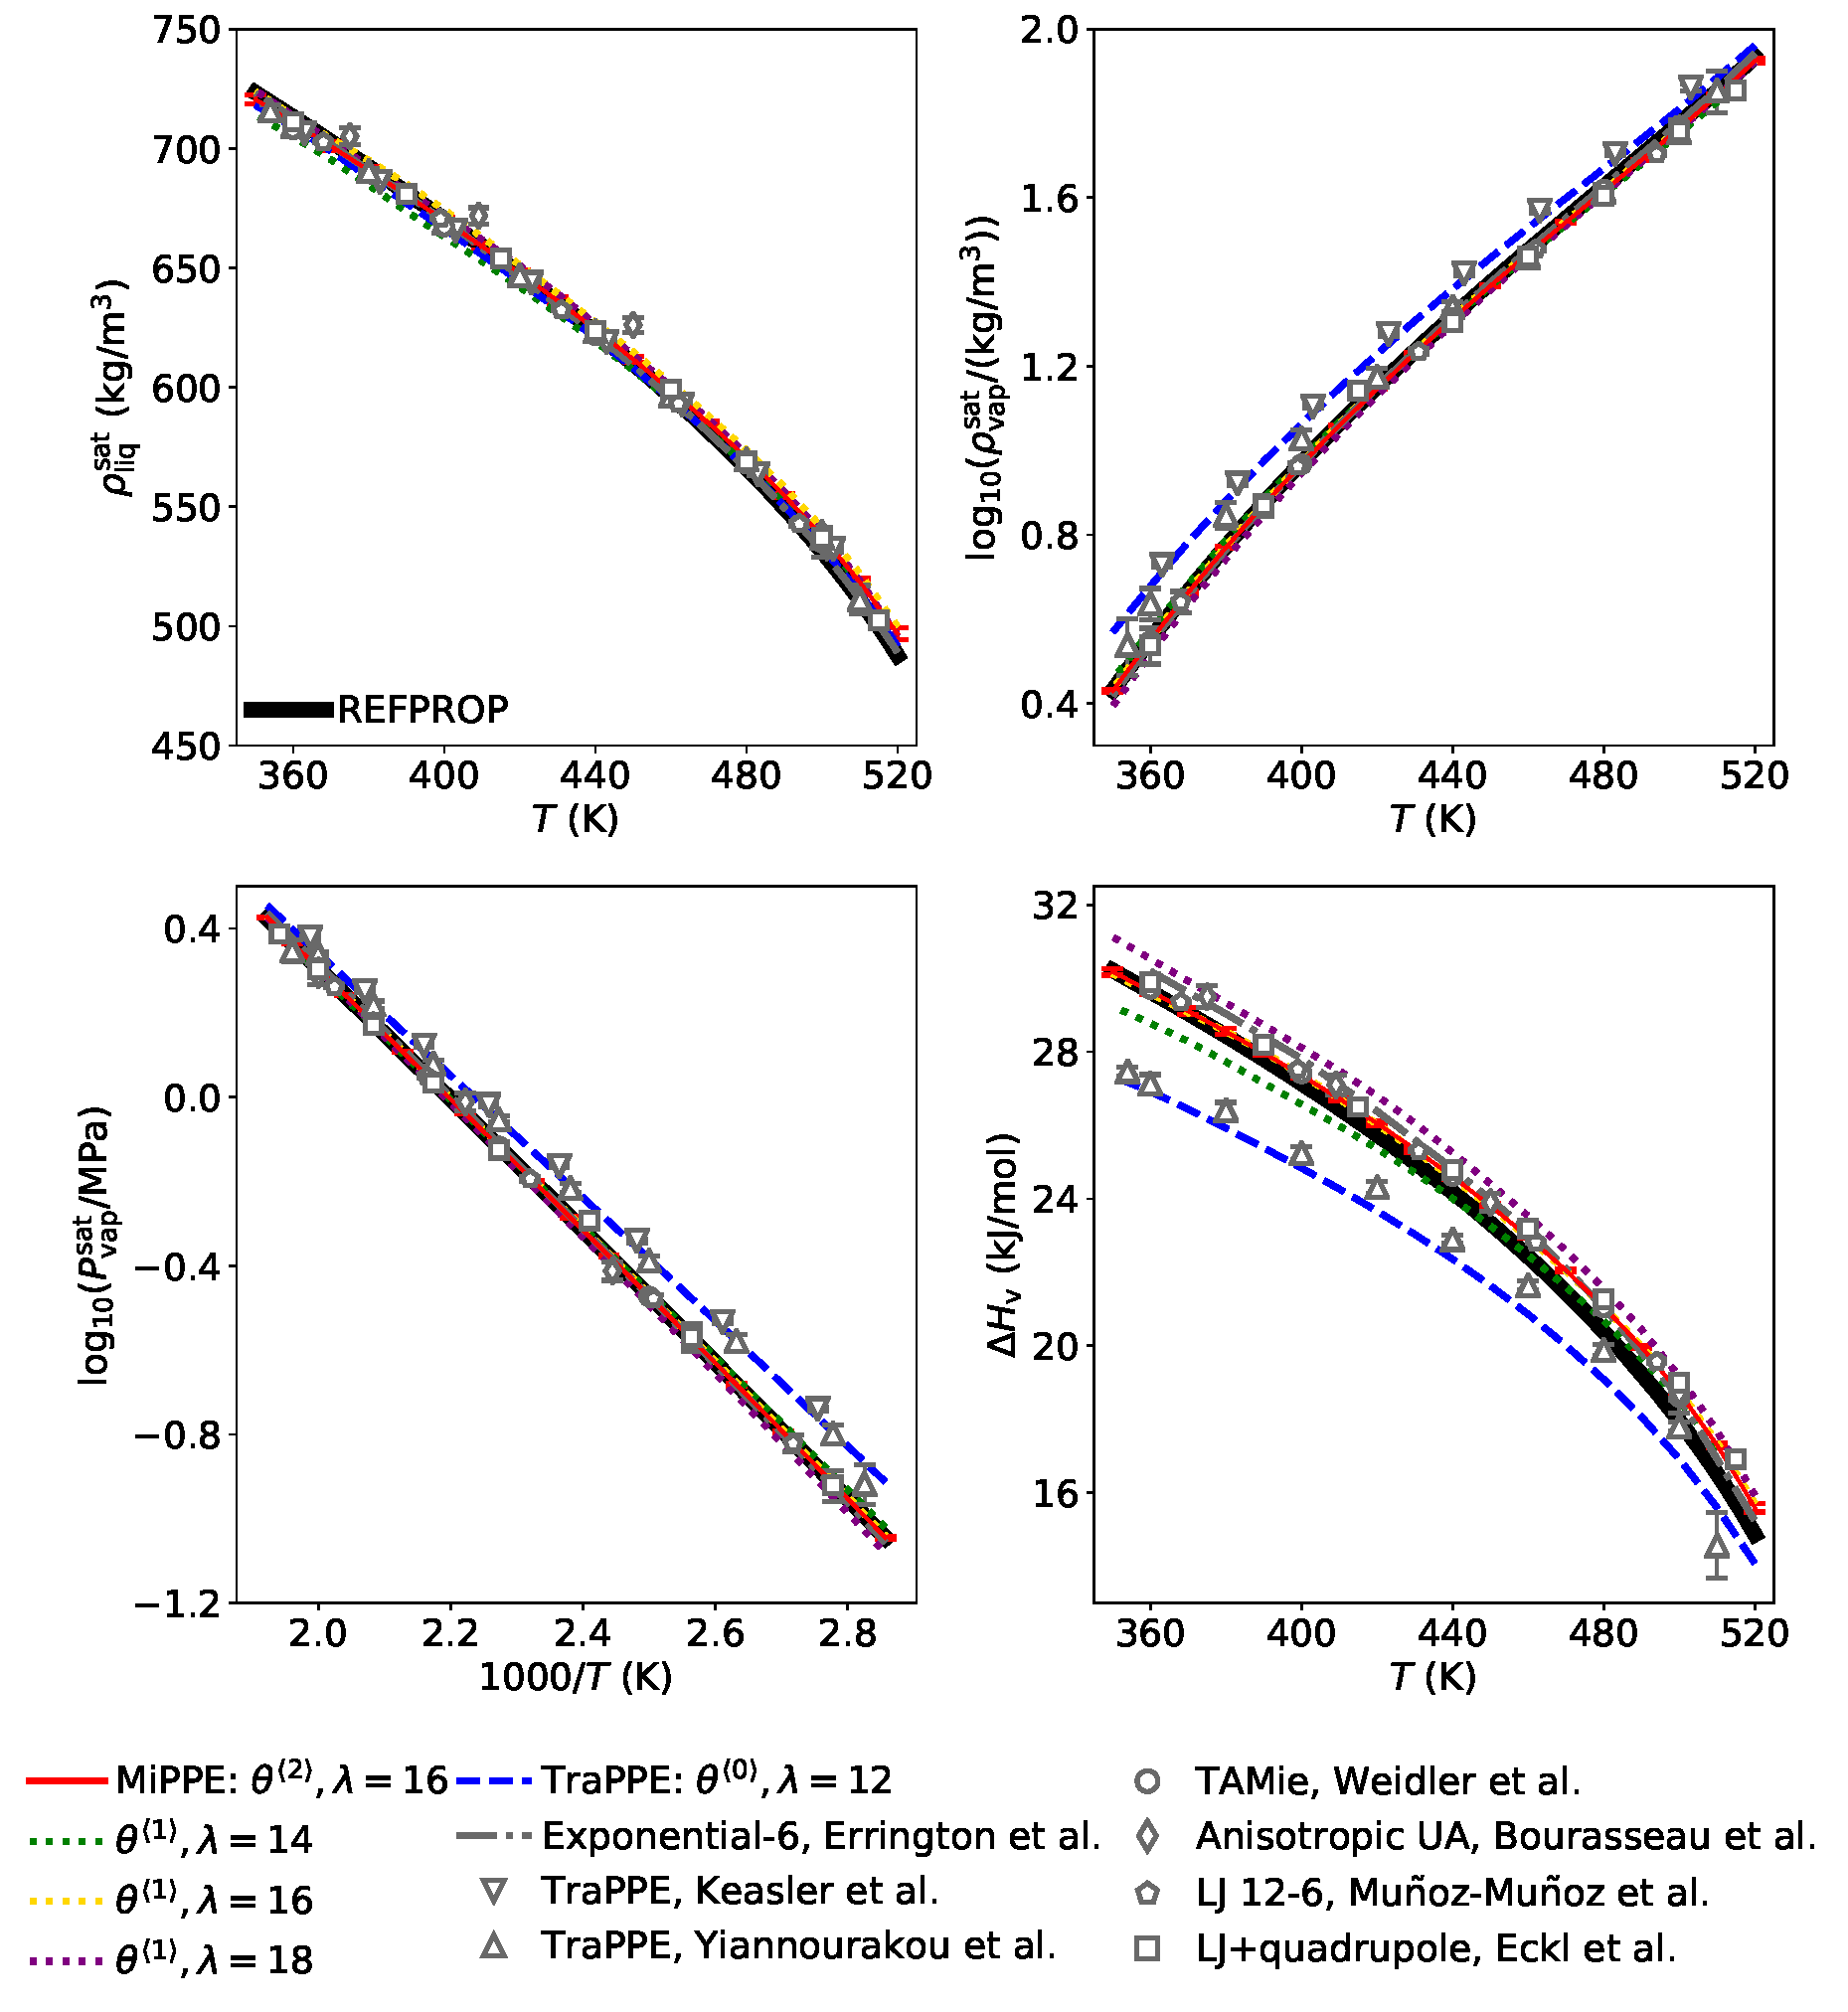
\includegraphics[width=5.8in]{CYC6_VLE_iterations.pdf}
		\caption{Phase equilibria for MiPPE ($\theta^{\langle2\rangle}, \lambda_{\rm CH_2} = 16$), zeroth iteration (TraPPE: $\theta^{\langle0\rangle}$), first iterations ($\theta^{\langle1\rangle}, \lambda_{\rm CH_2} = 14, 16, 18, 20$), and several literature force fields. See caption of Figure 9 in manuscript for details.}
		\label{SI fig: VLE cyclohexane}
	\end{figure}

\newpage
\clearpage

\subsection{Twenty replicates}

	\begin{figure}[H]
		\centering
		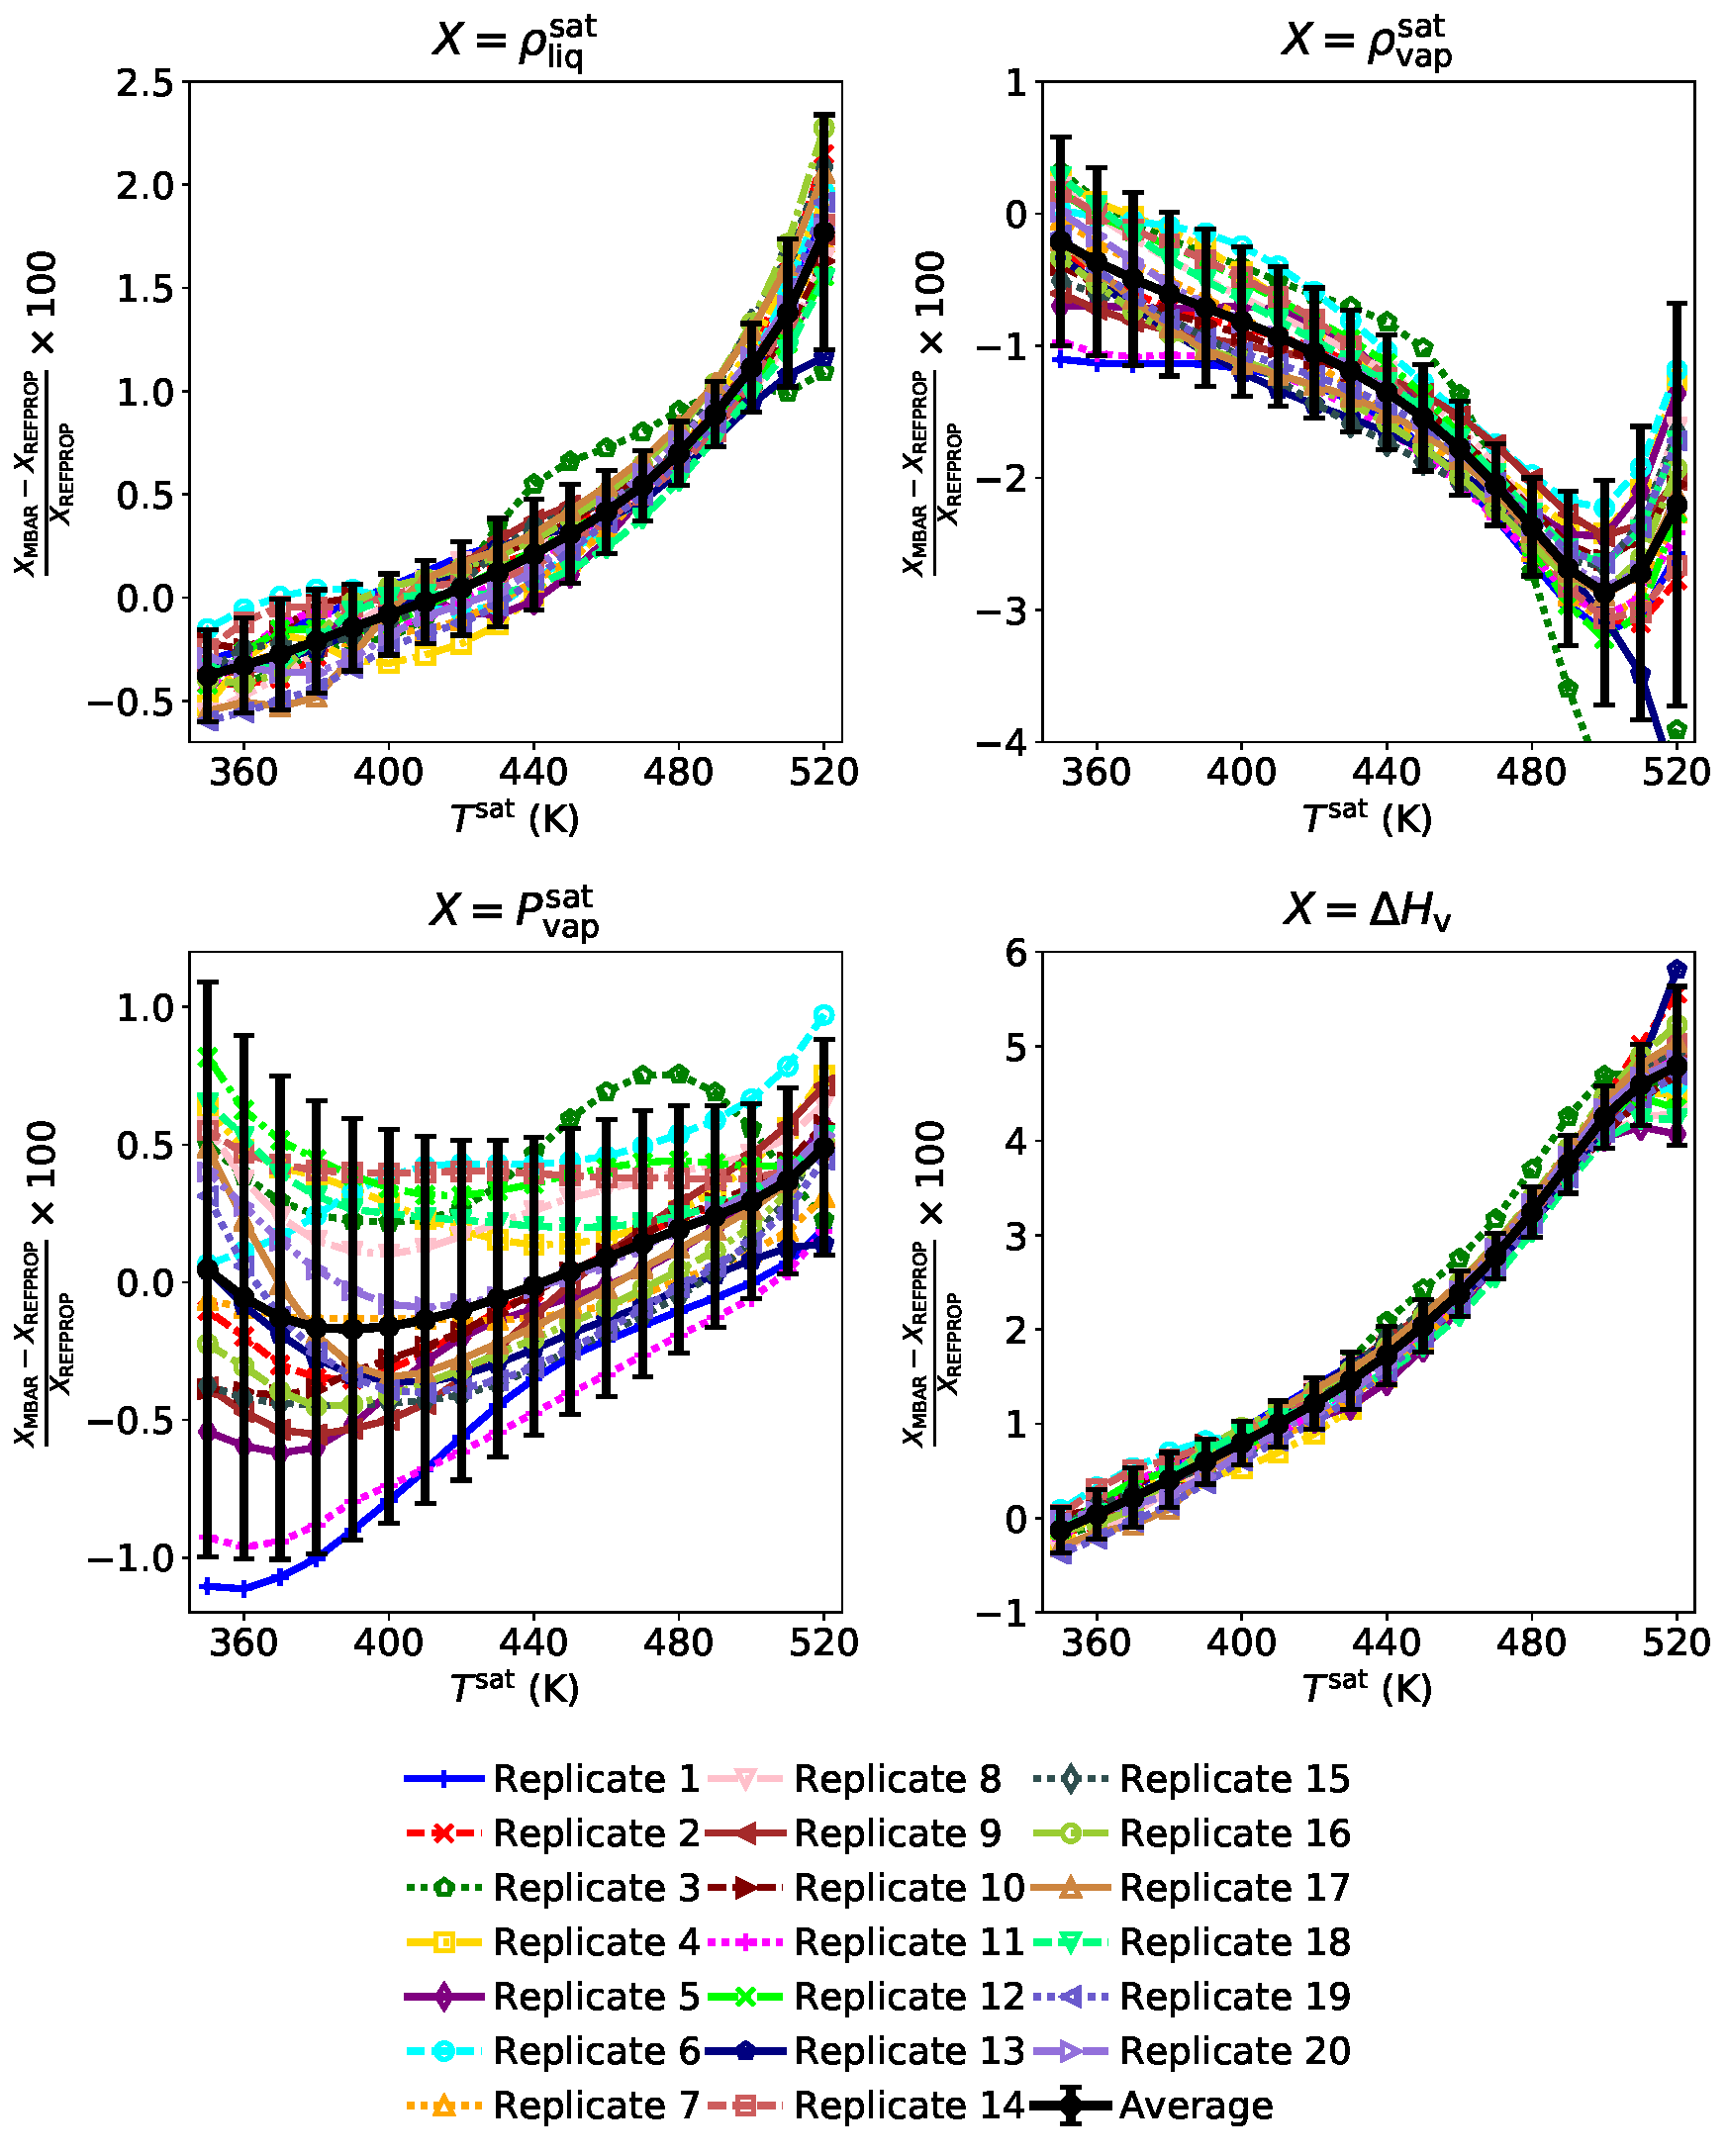
\includegraphics[width=5.8in]{CYC6_deviations_20replicates.pdf}
		\caption{Percent deviations of MiPPE force field relative to REFPROP cyclohexane values for twenty replicates and average.}
		\label{SI fig: VLE cyclohexane replicates}
	\end{figure}

\newpage
\clearpage

\subsection{TAMie comparison} \label{SI sec: TAMie comparison}

\begin{figure}[H]
	\centering
	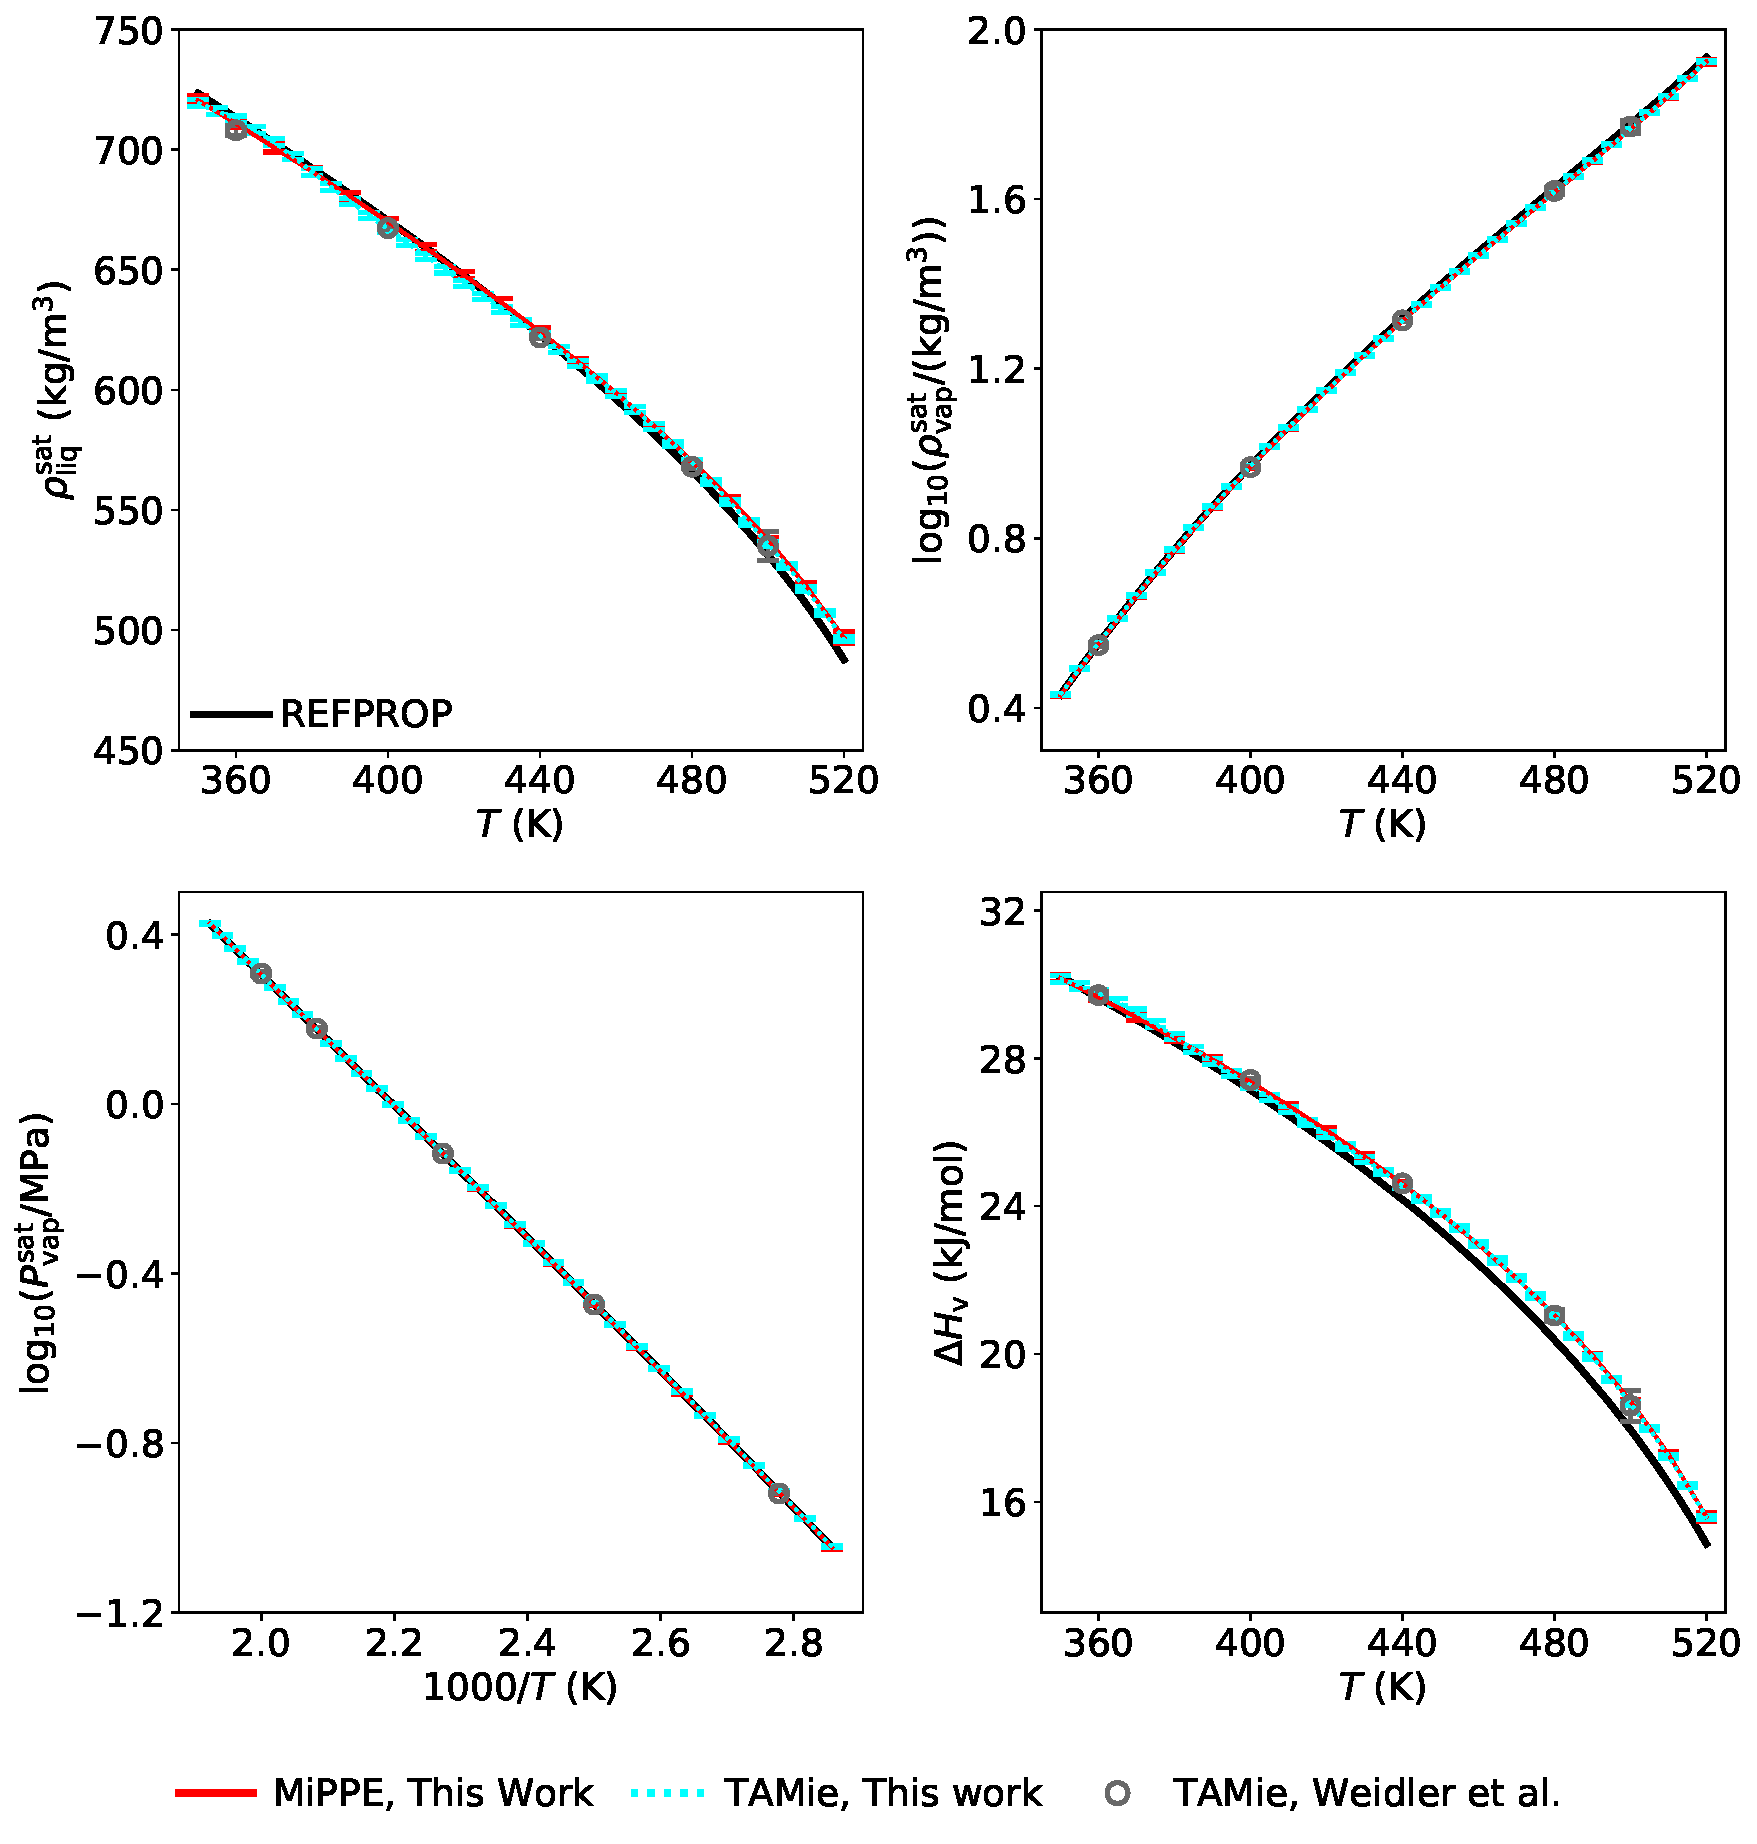
\includegraphics[width=5.8in]{CYC6_VLE_MiPPE_TAMie.pdf}
	\caption{Comparison of MiPPE and TAMie (from this work and Weidler et al.) cyclohexane phase equilibria. All simulations from this work utilized 3.5 nm box length. TAMie simulations used a 1.4 nm cut-off.}
	\label{SI fig: CYC6_VLE_MiPPE_TAMie}
\end{figure}

\begin{figure}[H]
	\centering
	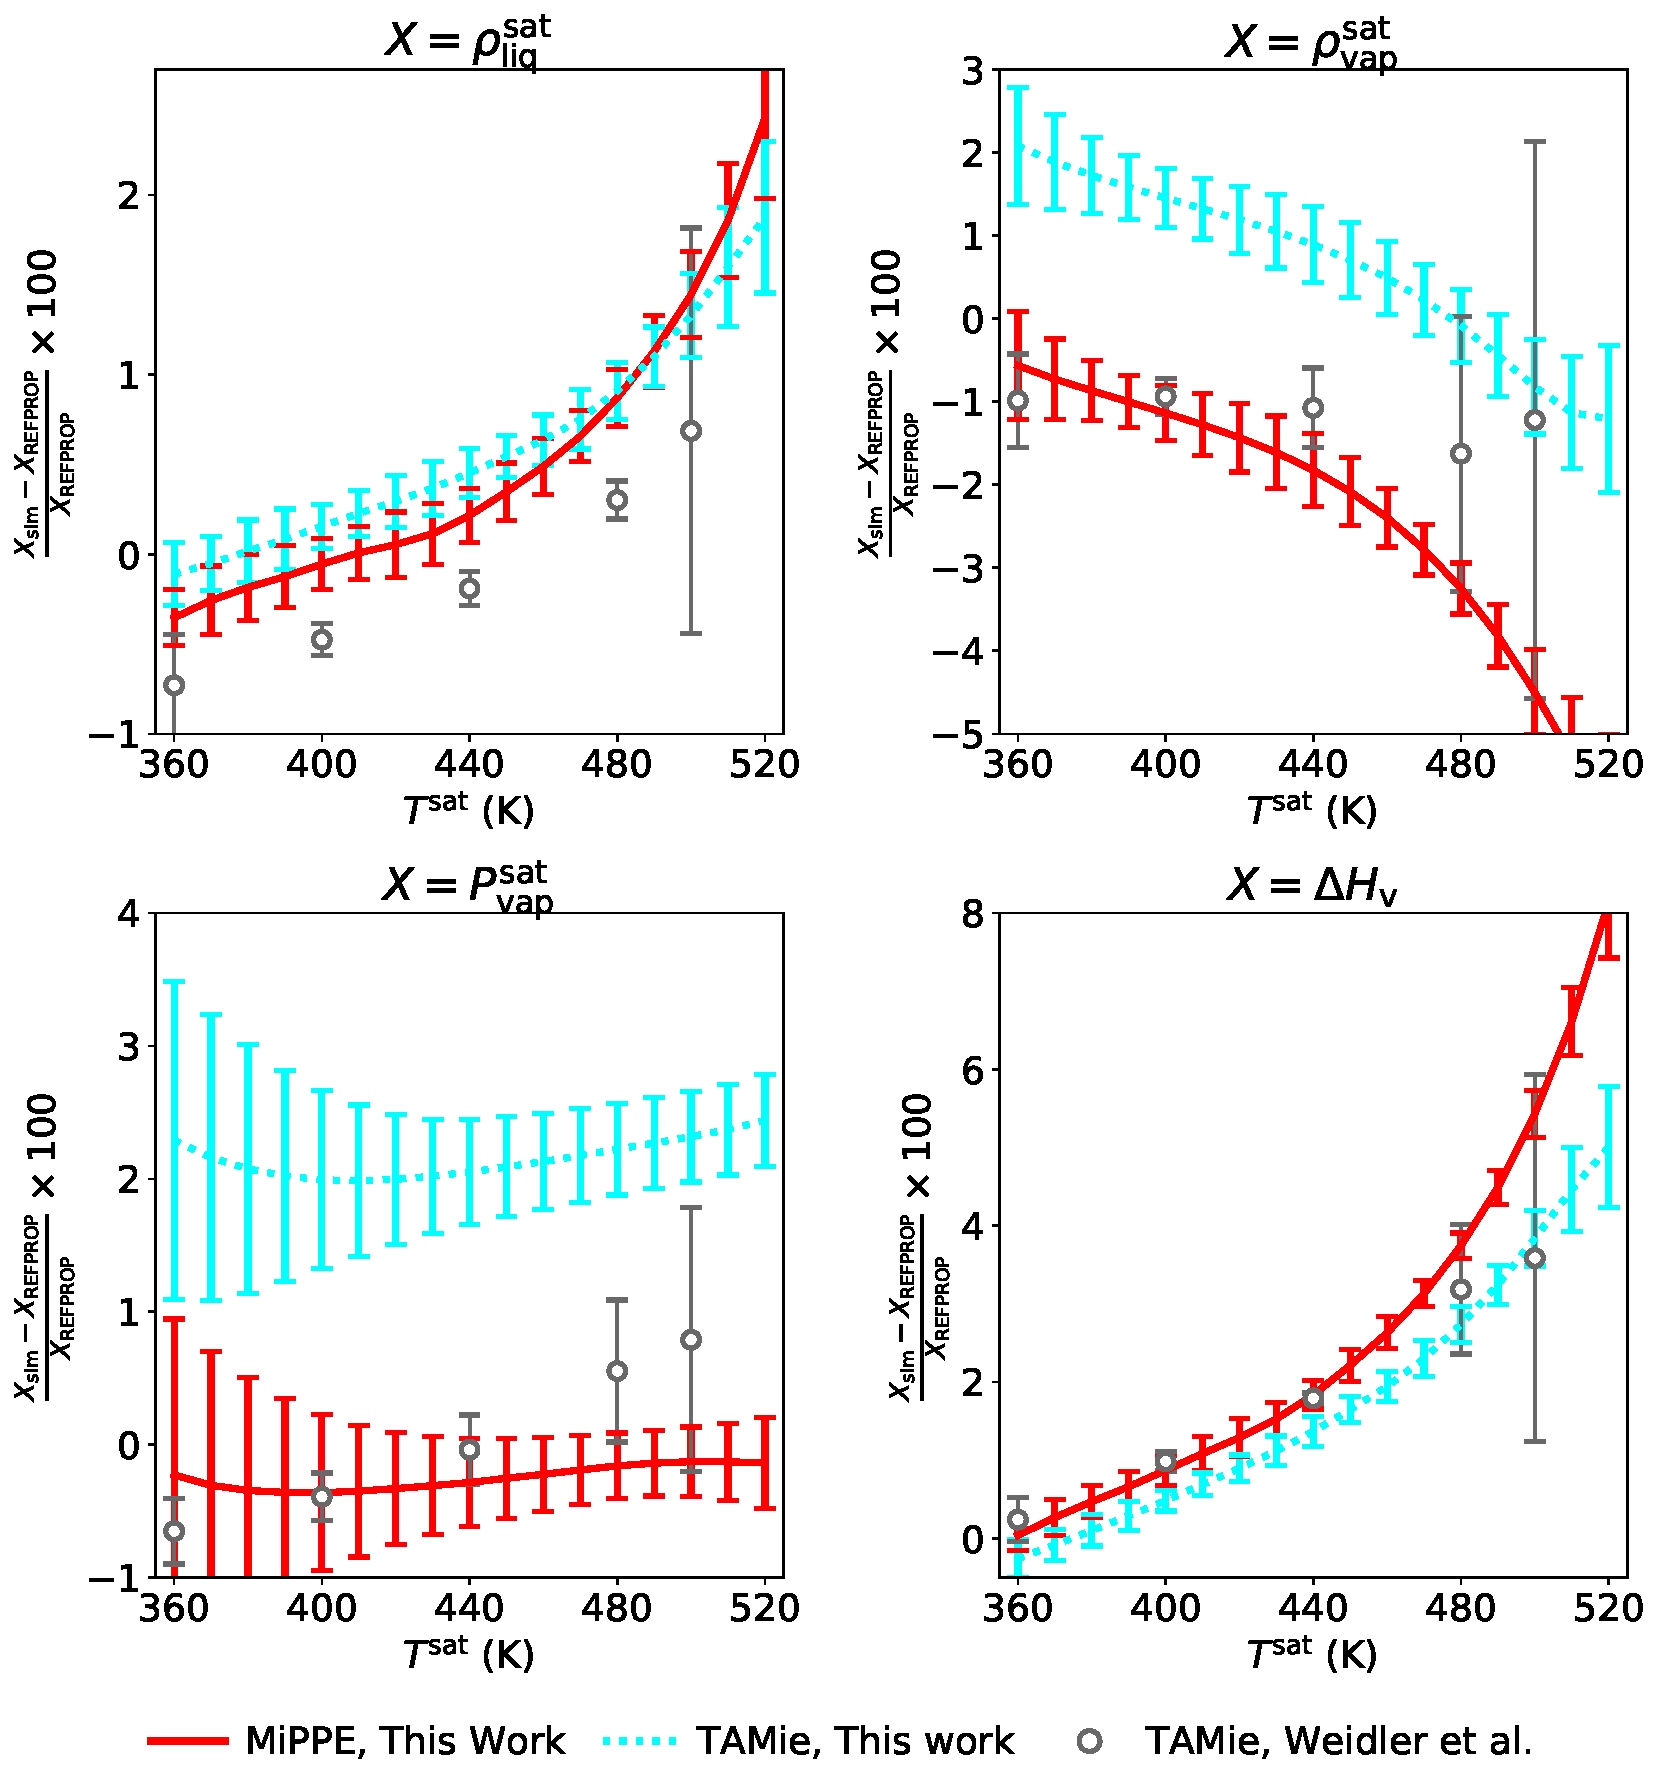
\includegraphics[width=5.8in]{CYC6_deviations_MiPPE_TAMie.pdf}
	\caption{Comparison of MiPPE and TAMie (from this work and Weidler et al.) deviations relative to REFPROP cyclohexane values. All simulations from this work utilized 3.5 nm box length. TAMie simulations used a 1.4 nm cut-off.}
	\label{SI fig: CYC6_deviations_MiPPE_TAMie}
\end{figure}

\newpage
\clearpage

\subsection{Minimum number of effective snapshots} \label{SI sec: Min eff}

\begin{figure}[htb!]
	\centering
	\includegraphics[width=6.4in]{CYC6_min_Neff_lam_iteration.pdf}
	\caption{Second iteration minimum number of effective snapshots $(\min(K_{\rm snaps}^{\rm eff}))$ with respect to $\epsilon_{\rm CH_2}$ and $\sigma_{\rm CH_2}$ for cyclohexane. Optimization has converged as $\min(K_{\rm snaps}^{\rm eff}) \gg 50$ for the optimal $\epsilon_{\rm CH_2}$, $\sigma_{\rm CH_2}$, $\lambda_{\rm CH_2}$ parameter set. Top-left, top-right, bottom-left, and bottom-right panels correspond $\lambda_{\rm CH_2} = 14$, $\lambda_{\rm CH_2} = 16$, $\lambda_{\rm CH_2} = 18$, and $\lambda_{\rm CH_2} = 12$, respectively. White star represents the optimal parameter set, i.e., the lowest value of $S$, for a given $\lambda_{\rm CH_2}$.}
	\label{SI fig:Iterate_Neff_CYC6}
\end{figure}

\newpage
\clearpage

\subsection{Finite-size effects} \label{SI sec: finite-size effects}

	\begin{figure}[H]
		\centering
		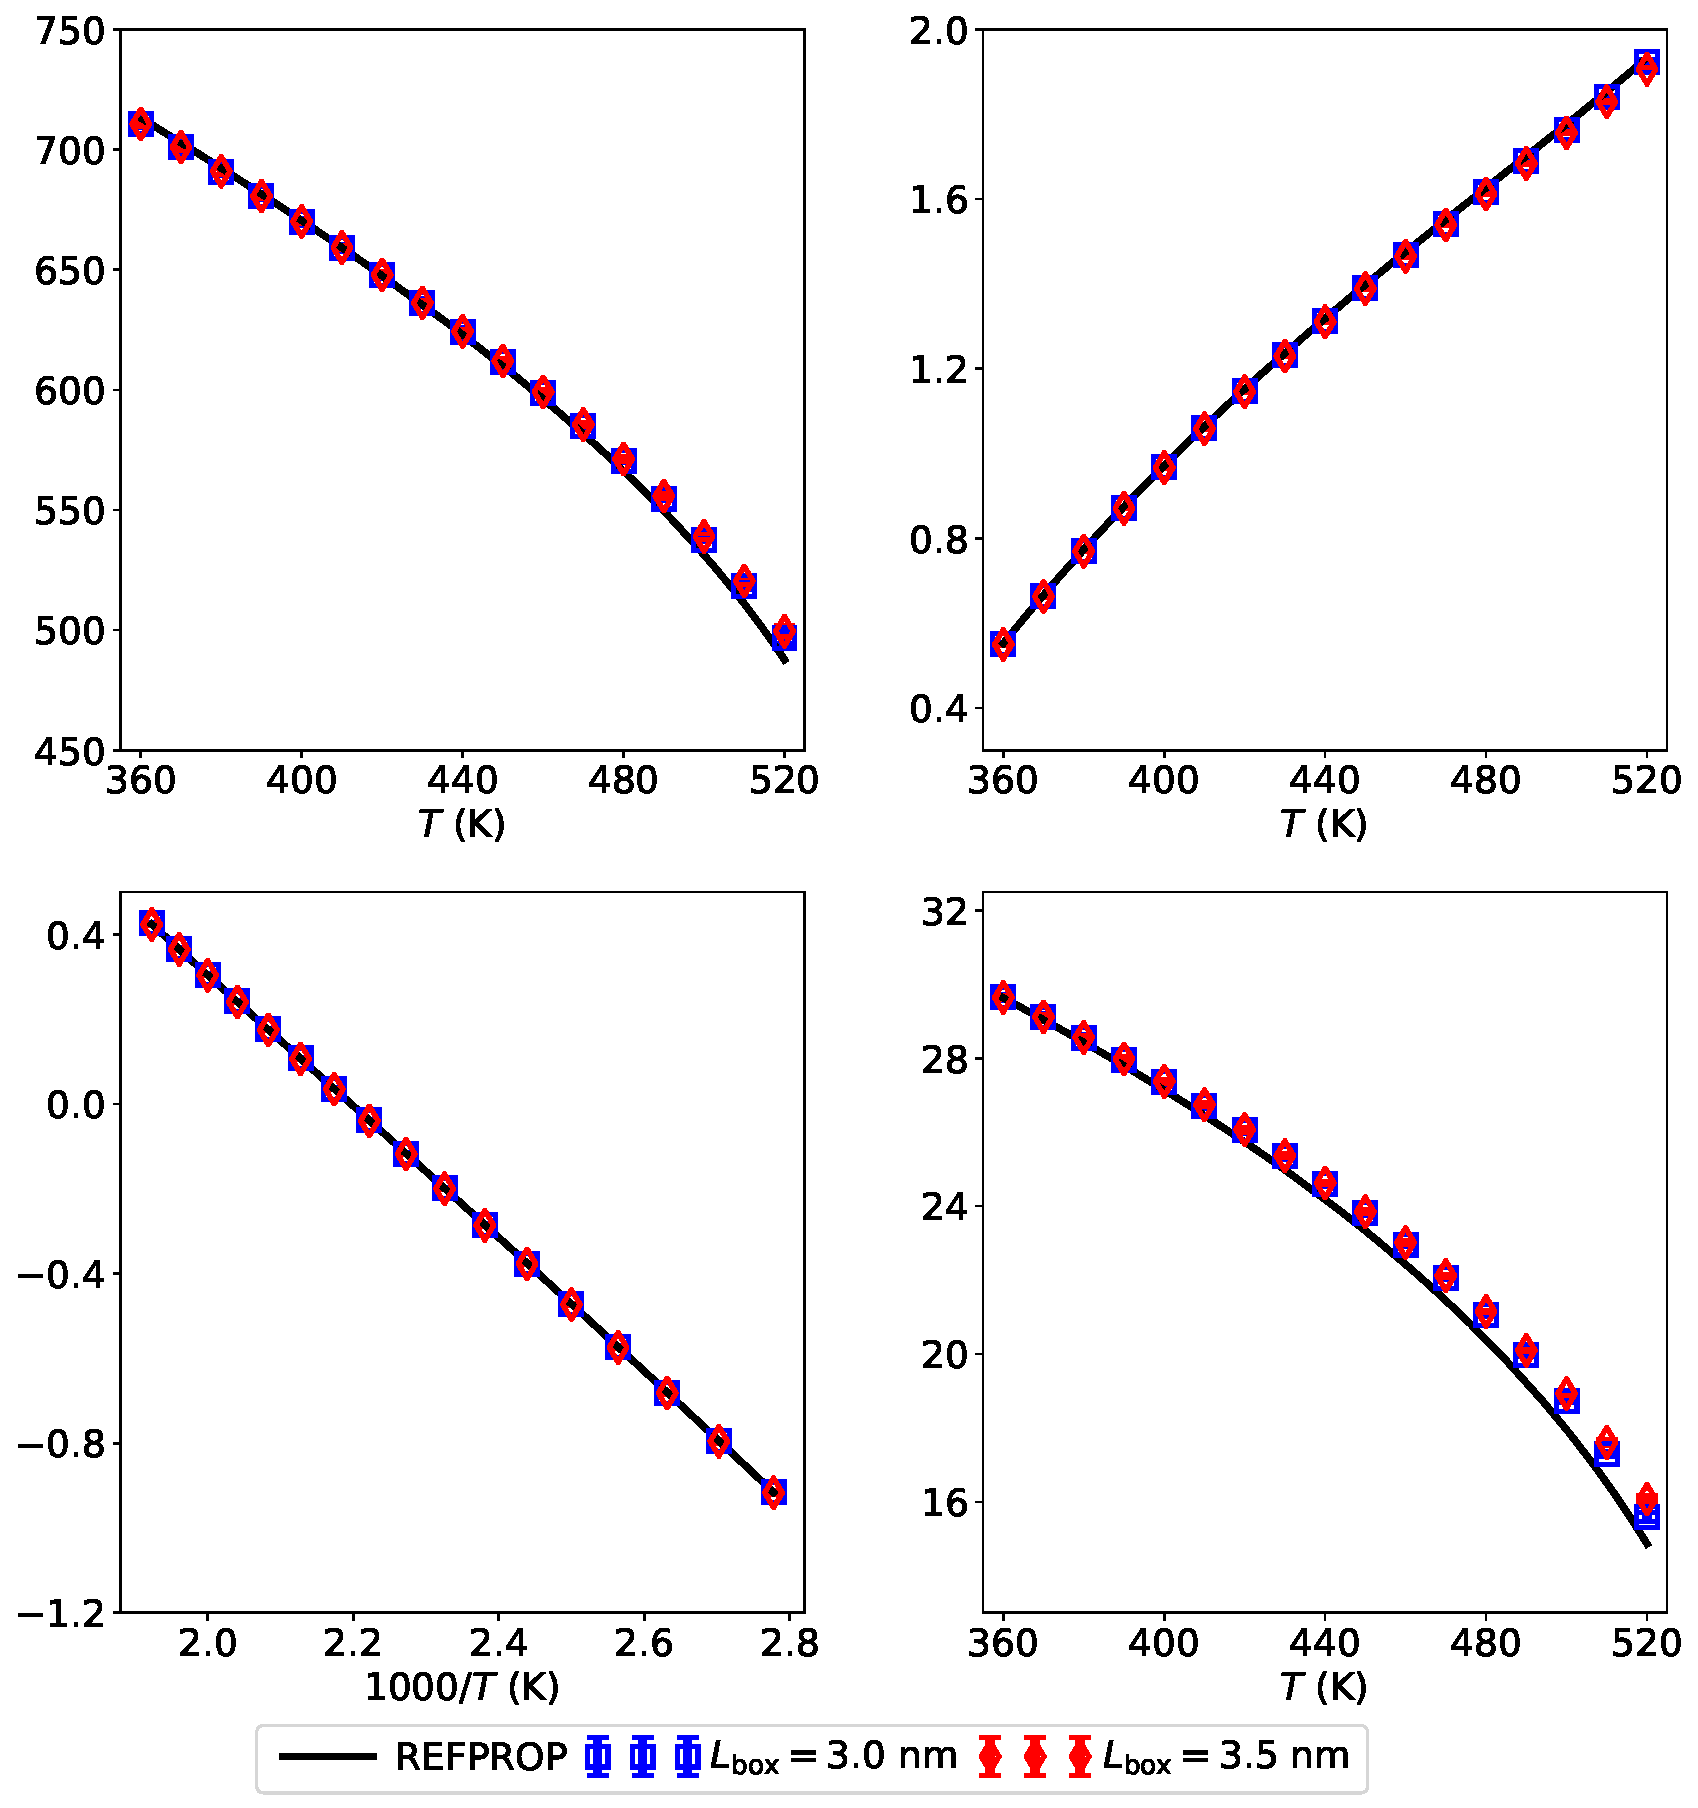
\includegraphics[width=5.8in]{CYC6_VLE_finite_size_effects.pdf}
		\caption{Comparison of phase equilibria using simulations with 3.0 nm and 3.5 nm box lengths for cyclohexane with MiPPE force field. Estimated values and uncertainties are obtained from 20 independent replicate simulations. See Figure \ref{SI fig:CYC6_finite_size_effects} for quantitative assessment of finite-size effects.}
		\label{SI fig: VLE CYC6_finite_size_effects}
	\end{figure}

	\newpage
	\clearpage

	\begin{figure}[H]
		\centering
		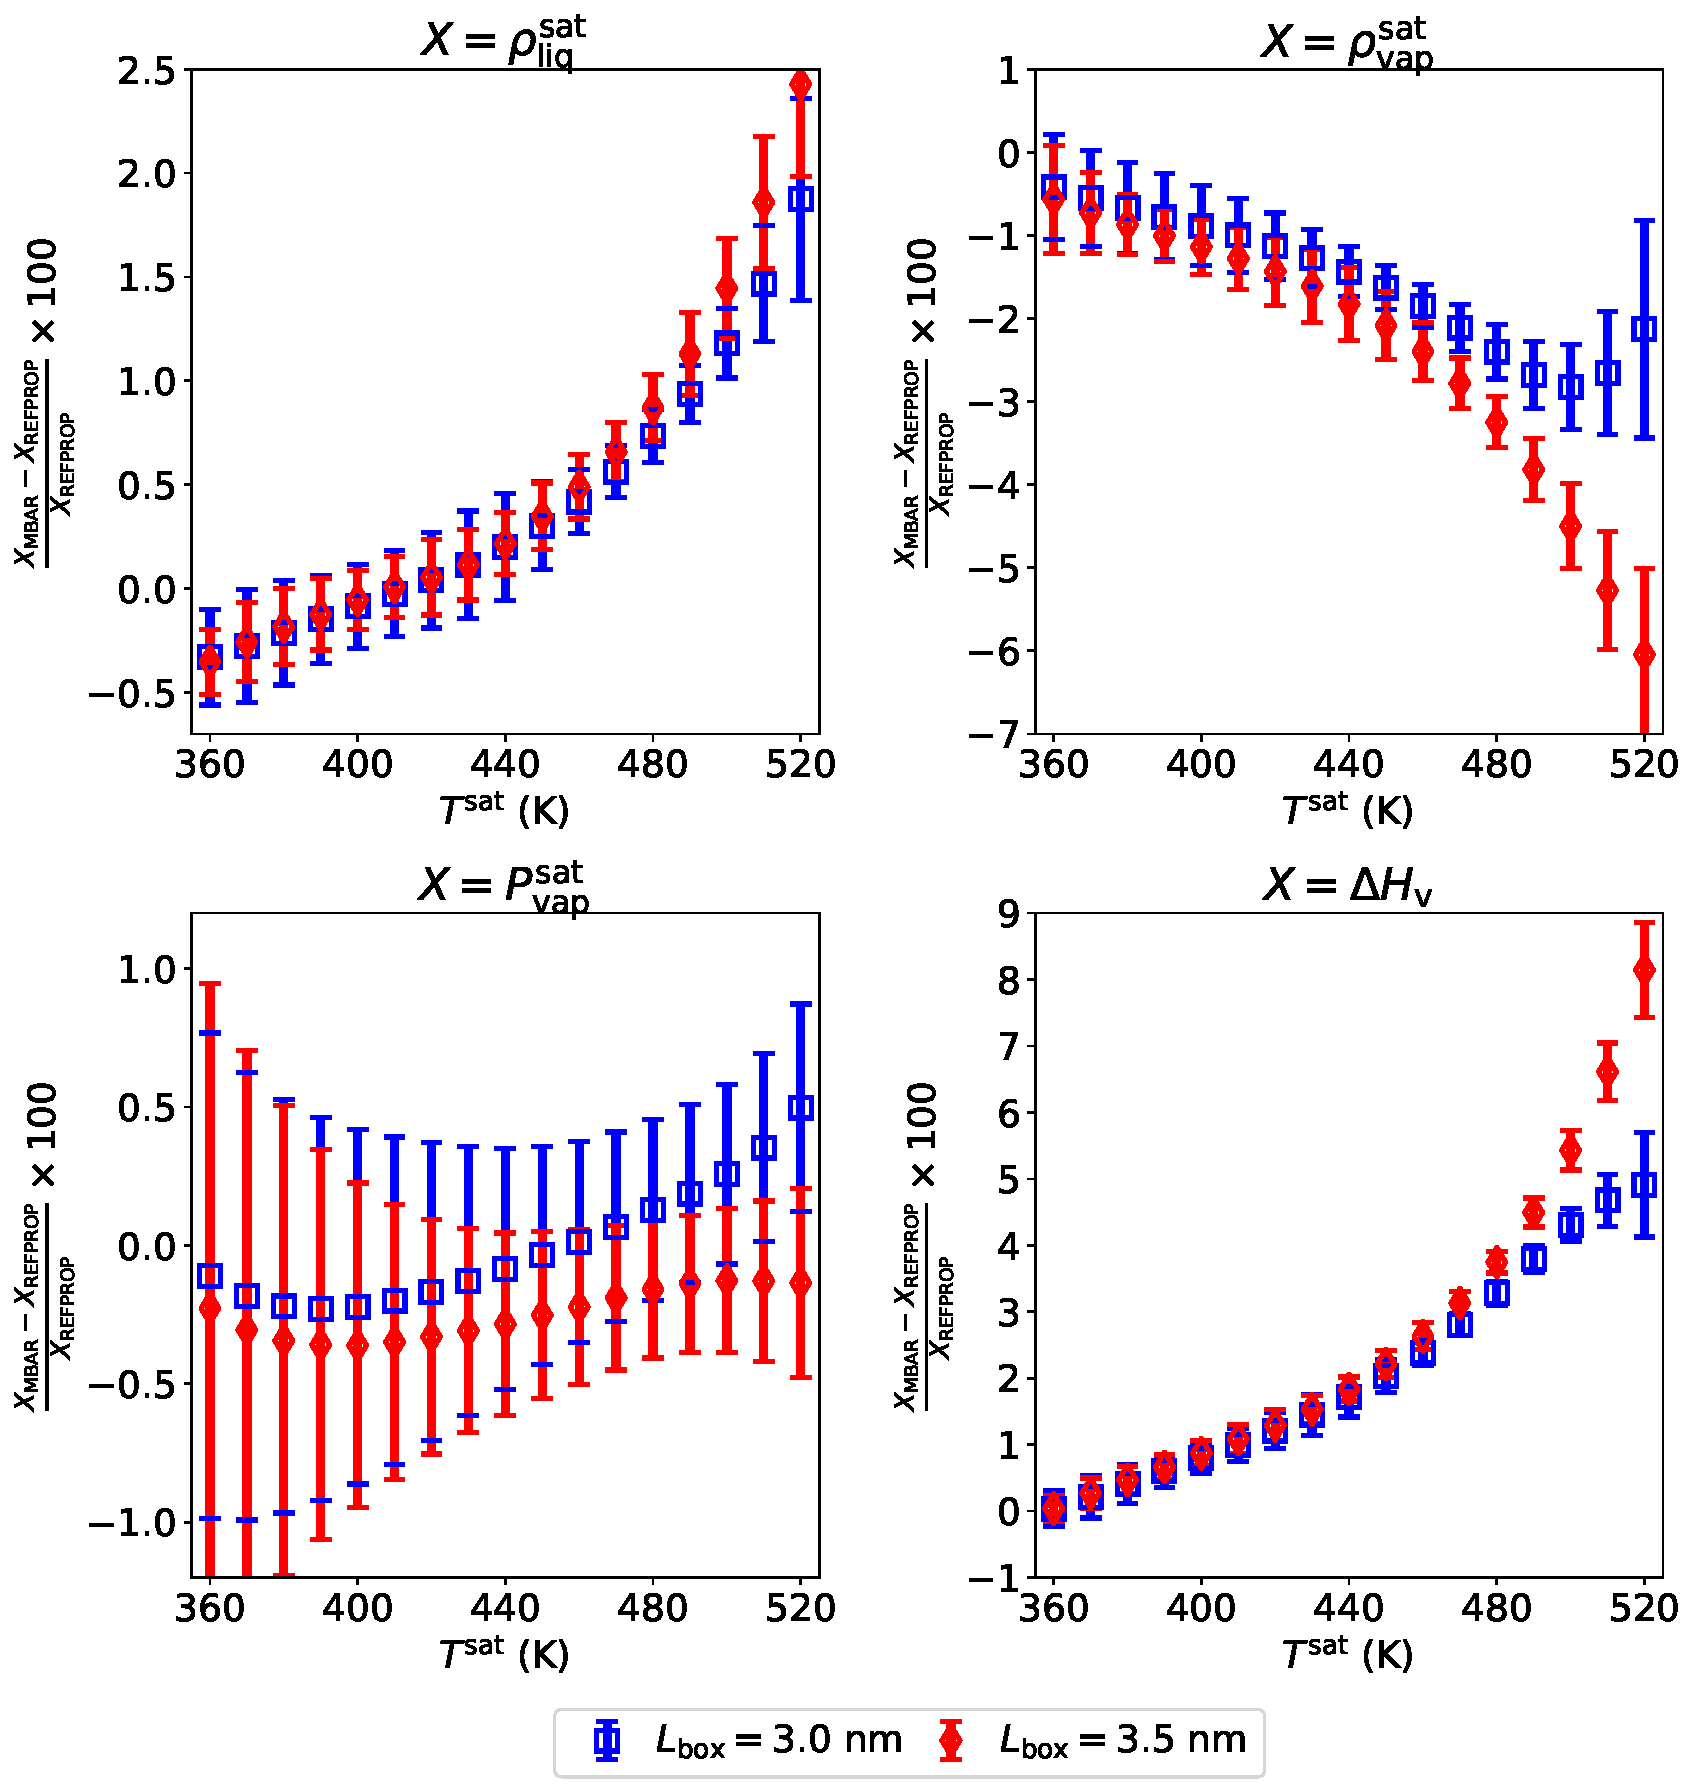
\includegraphics[width=5.8in]{CYC6_deviations_finite_size_effects.pdf}
		\caption{Comparison of percent deviations using simulations with 3.0 nm and 3.5 nm box lengths for cyclohexane with MiPPE force field. Agreement is typically within the combined uncertainties for low to moderate temperatures. Finite-size effects are most prevalent in $\rho_{\rm vap}^{\rm sat}$ and $\Delta H_{\rm v}$ near the critical temperature ($T^{\rm sat} > 480$ K). Estimated values and uncertainties are obtained from 20 independent replicate simulations.}
		\label{SI fig:CYC6_finite_size_effects}
	\end{figure}

	\newpage
	\clearpage

	\begin{table}[htb!]
		\caption{GCMC-MBAR results for the MiPPE force field with 3.5 nm box length to test finite-size effects. Subscripts correspond to the 95\% confidence interval computed with twenty independent replicate GCMC simulations at each state point.}
		\begin{center}
			\begin{tabular}{|c|c|c|c|c|c|}
				\hline
				$T^{\rm sat}$ (K) & $\rho_{\rm liq}^{\rm sat}$ (kg/m$^3$) & $\rho_{\rm vap}^{\rm sat}$ (kg/m$^3$) & $P_{\rm vap}^{\rm sat}$ (MPa) & $\Delta H_{\rm v}$ (kJ/mol) & $Z_{\rm vap}^{\rm sat}$ \\ \hline
				360 & $710.7_{1.2}$ & $3.545_{0.025}$ & $0.1211_{0.0015}$ & $29.648_{0.061}$ & $0.961_{0.014}$ \\
				370 & $701.0_{1.4}$ & $4.600_{0.024}$ & $0.1601_{0.0017}$ & $29.122_{0.071}$ & $0.952_{0.011}$ \\
				380 & $691.0_{1.4}$ & $5.882_{0.023}$ & $0.2081_{0.0019}$ & $28.567_{0.062}$ & $0.9424_{0.0093}$ \\
				390 & $680.7_{1.2}$ & $7.424_{0.025}$ & $0.2665_{0.0020}$ & $27.984_{0.057}$ & $0.9315_{0.0077}$ \\
				400 & $670.1_{1.0}$ & $9.261_{0.033}$ & $0.3365_{0.0021}$ & $27.379_{0.056}$ & $0.9195_{0.0067}$ \\
				410 & $659.2_{1.0}$ & $11.434_{0.046}$ & $0.4196_{0.0022}$ & $26.743_{0.060}$ & $0.9061_{0.0061}$ \\
				420 & $647.9_{1.3}$ & $13.987_{0.063}$ & $0.5173_{0.0023}$ & $26.070_{0.066}$ & $0.8913_{0.0057}$ \\
				430 & $636.2_{1.2}$ & $16.970_{0.081}$ & $0.6309_{0.0025}$ & $25.364_{0.057}$ & $0.8752_{0.0054}$ \\
				440 & $624.3_{1.0}$ & $20.444_{0.098}$ & $0.7621_{0.0027}$ & $24.627_{0.047}$ & $0.8576_{0.0051}$ \\
				450 & $612.1_{1.0}$ & $24.48_{0.11}$ & $0.9125_{0.0029}$ & $23.849_{0.050}$ & $0.8385_{0.0046}$ \\
				460 & $599.17_{0.99}$ & $29.16_{0.11}$ & $1.0837_{0.0032}$ & $23.015_{0.049}$ & $0.8178_{0.0040}$ \\
				470 & $585.58_{0.89}$ & $34.59_{0.12}$ & $1.2774_{0.0036}$ & $22.120_{0.039}$ & $0.7953_{0.0035}$ \\
				480 & $571.22_{0.96}$ & $40.91_{0.14}$ & $1.4953_{0.0040}$ & $21.154_{0.035}$ & $0.7707_{0.0033}$ \\
				490 & $555.8_{1.2}$ & $48.31_{0.20}$ & $1.7394_{0.0046}$ & $20.099_{0.045}$ & $0.7438_{0.0037}$ \\
				500 & $539.0_{1.4}$ & $57.04_{0.33}$ & $2.0115_{0.0056}$ & $18.930_{0.057}$ & $0.7139_{0.0045}$ \\
				510 & $520.5_{1.7}$ & $67.54_{0.54}$ & $2.3139_{0.0072}$ & $17.610_{0.076}$ & $0.6799_{0.0058}$ \\
				520 & $499.5_{2.3}$ & $80.59_{0.95}$ & $2.6492_{0.0097}$ & $16.07_{0.11}$ & $0.6399_{0.0079}$ \\
				\hline
			\end{tabular}
		\end{center}
	\end{table}

\newpage
\clearpage

\subsection{Tabulated phase equilibria for iterations}

	\begin{table}[htb!]
		\caption{GCMC-MBAR results for the MiPPE force field (second iteration, $\theta^{\langle2\rangle}$ $\lambda_{\rm CH_2} = 16$). Subscripts correspond to the 95\% confidence interval computed with twenty independent replicate GCMC simulations at each state point.}
		\begin{center}
			\begin{tabular}{|c|c|c|c|c|c|}
				\hline
				$T^{\rm sat}$ (K) & $\rho_{\rm liq}^{\rm sat}$ (kg/m$^3$) & $\rho_{\rm vap}^{\rm sat}$ (kg/m$^3$) & $P_{\rm vap}^{\rm sat}$ (MPa) & $\Delta H_{\rm v}$ (kJ/mol) & $Z_{\rm vap}^{\rm sat}$ \\ \hline
				360 & $710.9_{1.7}$ & $3.552_{0.027}$ & $0.1213_{0.0012}$ & $29.648_{0.084}$ & $0.960_{0.012}$ \\
				370 & $700.9_{2.0}$ & $4.611_{0.032}$ & $0.1604_{0.0015}$ & $29.106_{0.098}$ & $0.952_{0.011}$ \\
				380 & $690.8_{1.8}$ & $5.898_{0.039}$ & $0.2085_{0.0018}$ & $28.548_{0.088}$ & $0.942_{0.010}$ \\
				390 & $680.5_{1.5}$ & $7.446_{0.048}$ & $0.2670_{0.0022}$ & $27.967_{0.071}$ & $0.9306_{0.0097}$ \\
				400 & $669.9_{1.4}$ & $9.291_{0.056}$ & $0.3372_{0.0026}$ & $27.359_{0.067}$ & $0.9183_{0.0090}$ \\
				410 & $659.0_{1.4}$ & $11.474_{0.065}$ & $0.4205_{0.0030}$ & $26.720_{0.069}$ & $0.9048_{0.0083}$ \\
				420 & $647.8_{1.6}$ & $14.040_{0.075}$ & $0.5185_{0.0034}$ & $26.050_{0.074}$ & $0.8899_{0.0075}$ \\
				430 & $636.3_{1.8}$ & $17.043_{0.085}$ & $0.6325_{0.0039}$ & $25.346_{0.082}$ & $0.8736_{0.0069}$ \\
				440 & $624.3_{1.8}$ & $20.543_{0.096}$ & $0.7642_{0.0044}$ & $24.600_{0.080}$ & $0.8558_{0.0064}$ \\
				450 & $611.8_{1.6}$ & $24.61_{0.11}$ & $0.9152_{0.0051}$ & $23.807_{0.069}$ & $0.8363_{0.0059}$ \\
				460 & $598.7_{1.3}$ & $29.35_{0.11}$ & $1.0871_{0.0058}$ & $22.958_{0.058}$ & $0.8151_{0.0054}$ \\
				470 & $584.9_{1.1}$ & $34.85_{0.12}$ & $1.2816_{0.0066}$ & $22.044_{0.055}$ & $0.7920_{0.0049}$ \\
				480 & $570.25_{0.93}$ & $41.29_{0.17}$ & $1.5006_{0.0072}$ & $21.051_{0.058}$ & $0.7665_{0.0048}$ \\
				490 & $554.49_{0.93}$ & $48.88_{0.31}$ & $1.7460_{0.0075}$ & $19.956_{0.063}$ & $0.7379_{0.0057}$ \\
				500 & $537.3_{1.2}$ & $58.02_{0.54}$ & $2.0200_{0.0076}$ & $18.718_{0.064}$ & $0.7049_{0.0071}$ \\
				510 & $518.0_{2.0}$ & $69.36_{0.85}$ & $2.3254_{0.0084}$ & $17.276_{0.076}$ & $0.6654_{0.0085}$ \\
				520 & $496.3_{3.0}$ & $83.9_{1.4}$ & $2.666_{0.011}$ & $15.58_{0.13}$ & $0.619_{0.011}$ \\
				\hline
			\end{tabular}
		\end{center}
	\end{table}

	\begin{table}[htb!]
		\caption{GCMC-MBAR results for the TraPPE force field (zeroth iteration, $\theta^{\langle0\rangle})$. Subscripts correspond to the 95\% confidence interval computed with bootstrap re-sampling.}
		\begin{center}
			\begin{tabular}{|c|c|c|c|c|c|}
				\hline
				$T^{\rm sat}$ (K) & $\rho_{\rm liq}^{\rm sat}$ (kg/m$^3$) & $\rho_{\rm vap}^{\rm sat}$ (kg/m$^3$) & $P_{\rm vap}^{\rm sat}$ (MPa) & $\Delta H_{\rm v}$ (kJ/mol) & $Z_{\rm vap}^{\rm sat}$ \\ \hline
				360 & $709.02_{0.33}$ & $4.775_{0.062}$ & $0.161_{0.016}$ & $26.916_{0.050}$ & $0.946_{0.096}$ \\
				370 & $698.93_{0.39}$ & $6.067_{0.072}$ & $0.208_{0.012}$ & $26.440_{0.042}$ & $0.937_{0.055}$ \\
				380 & $688.03_{0.44}$ & $7.610_{0.088}$ & $0.26_{0.01}$ & $25.919_{0.036}$ & $0.927_{0.026}$ \\
				390 & $677.14_{0.49}$ & $9.43_{0.11}$ & $0.33_{0.01}$ & $25.382_{0.033}$ & $0.916_{0.015}$ \\
				400 & $666.43_{0.55}$ & $11.57_{0.12}$ & $0.41_{0.01}$ & $24.835_{0.030}$ & $0.904_{0.023}$ \\
				410 & $655.56_{0.39}$ & $14.07_{0.13}$ & $0.507_{0.017}$ & $24.266_{0.023}$ & $0.890_{0.032}$ \\
				420 & $644.33_{0.48}$ & $16.97_{0.13}$ & $0.616_{0.025}$ & $23.665_{0.027}$ & $0.875_{0.036}$ \\
				430 & $632.76_{0.54}$ & $20.32_{0.12}$ & $0.741_{0.031}$ & $23.030_{0.030}$ & $0.858_{0.037}$ \\
				440 & $620.79_{0.67}$ & $24.18_{0.26}$ & $0.883_{0.039}$ & $22.356_{0.051}$ & $0.840_{0.038}$ \\
				450 & $608.2_{1.2}$ & $28.64_{0.96}$ & $1.045_{0.052}$ & $21.63_{0.10}$ & $0.821_{0.049}$ \\
				460 & $595.0_{2.9}$ & $33.8_{2.4}$ & $1.227_{0.098}$ & $20.85_{0.20}$ & $0.799_{0.085}$ \\
				470 & $581.0_{4.6}$ & $39.7_{3.8}$ & $1.43_{0.17}$ & $20.01_{0.30}$ & $0.78_{0.12}$ \\
				480 & $566.2_{4.8}$ & $46.7_{4.6}$ & $1.66_{0.24}$ & $19.08_{0.33}$ & $0.75_{0.13}$ \\
				490 & $550.4_{4.5}$ & $54.8_{4.7}$ & $1.91_{0.29}$ & $18.06_{0.38}$ & $0.72_{0.13}$ \\
				500 & $533.2_{5.4}$ & $64.6_{3.8}$ & $2.19_{0.38}$ & $16.913_{0.088}$ & $0.69_{0.13}$ \\
				510 & $513.8_{5.3}$ & $76.6_{5.4}$ & $2.50_{0.37}$ & $15.59_{0.33}$ & $0.65_{0.11}$ \\
				520 & $491.6_{3.8}$ & $91.4_{7.6}$ & $2.85_{0.28}$ & $14.08_{0.34}$ & $0.607_{0.078}$ \\
				\hline
			\end{tabular}
		\end{center}
	\end{table}

	\begin{table}[htb!]
		\caption{GCMC-MBAR results for the first iteration $(\theta^{\langle1\rangle})$ $\lambda_{\rm CH_2} = 14$ force field. Subscripts correspond to the 95\% confidence interval computed with bootstrap re-sampling.}
		\begin{center}
			\begin{tabular}{|c|c|c|c|c|c|}
				\hline
				$T^{\rm sat}$ (K) & $\rho_{\rm liq}^{\rm sat}$ (kg/m$^3$) & $\rho_{\rm vap}^{\rm sat}$ (kg/m$^3$) & $P_{\rm vap}^{\rm sat}$ (MPa) & $\Delta H_{\rm v}$ (kJ/mol) & $Z_{\rm vap}^{\rm sat}$ \\ \hline
				360 & $704.93_{0.26}$ & $3.743_{0.073}$ & $0.127_{0.044}$ & $28.78_{0.10}$ & $0.96_{0.33}$ \\
				370 & $695.36_{0.63}$ & $4.822_{0.057}$ & $0.167_{0.048}$ & $28.28_{0.11}$ & $0.95_{0.27}$ \\
				380 & $684.68_{0.79}$ & $6.125_{0.057}$ & $0.216_{0.049}$ & $27.73_{0.11}$ & $0.94_{0.21}$ \\
				390 & $673.71_{0.68}$ & $7.680_{0.084}$ & $0.274_{0.048}$ & $27.144_{0.099}$ & $0.93_{0.16}$ \\
				400 & $663.17_{0.45}$ & $9.52_{0.13}$ & $0.345_{0.044}$ & $26.568_{0.086}$ & $0.92_{0.12}$ \\
				410 & $652.73_{0.24}$ & $11.68_{0.17}$ & $0.427_{0.039}$ & $25.980_{0.062}$ & $0.903_{0.084}$ \\
				420 & $641.98_{0.82}$ & $14.21_{0.23}$ & $0.524_{0.033}$ & $25.360_{0.039}$ & $0.889_{0.058}$ \\
				430 & $630.8_{1.2}$ & $17.15_{0.30}$ & $0.636_{0.032}$ & $24.703_{0.036}$ & $0.873_{0.046}$ \\
				440 & $619.3_{1.1}$ & $20.57_{0.39}$ & $0.765_{0.041}$ & $24.005_{0.044}$ & $0.856_{0.049}$ \\
				450 & $607.24_{0.80}$ & $24.53_{0.54}$ & $0.912_{0.062}$ & $23.261_{0.063}$ & $0.837_{0.060}$ \\
				460 & $594.62_{0.73}$ & $29.11_{0.77}$ & $1.080_{0.093}$ & $22.463_{0.085}$ & $0.816_{0.074}$ \\
				470 & $581.33_{0.87}$ & $34.4_{1.1}$ & $1.27_{0.14}$ & $21.60_{0.11}$ & $0.793_{0.091}$ \\
				480 & $567.3_{1.1}$ & $40.6_{1.6}$ & $1.48_{0.21}$ & $20.68_{0.13}$ & $0.77_{0.11}$ \\
				490 & $552.4_{1.5}$ & $47.9_{2.1}$ & $1.72_{0.30}$ & $19.66_{0.14}$ & $0.74_{0.13}$ \\
				500 & $536.3_{2.5}$ & $56.5_{2.6}$ & $1.98_{0.41}$ & $18.52_{0.14}$ & $0.71_{0.15}$ \\
				510 & $518.2_{4.3}$ & $67.2_{2.8}$ & $2.27_{0.54}$ & $17.20_{0.16}$ & $0.67_{0.16}$ \\
				\hline
			\end{tabular}
		\end{center}
	\end{table}

	\begin{table}[htb!]
		\caption{GCMC-MBAR results for the first iteration $(\theta^{\langle1\rangle})$ $\lambda_{\rm CH_2} = 16$ force field. Subscripts correspond to the 95\% confidence interval computed with bootstrap re-sampling.}
		\begin{center}
			\begin{tabular}{|c|c|c|c|c|c|}
				\hline
				$T^{\rm sat}$ (K) & $\rho_{\rm liq}^{\rm sat}$ (kg/m$^3$) & $\rho_{\rm vap}^{\rm sat}$ (kg/m$^3$) & $P_{\rm vap}^{\rm sat}$ (MPa) & $\Delta H_{\rm v}$ (kJ/mol) & $Z_{\rm vap}^{\rm sat}$ \\ \hline
				360 & $713.64_{0.38}$ & $3.583_{0.049}$ & $0.122_{0.039}$ & $29.59_{0.13}$ & $0.96_{0.31}$ \\
				370 & $704.1_{1.2}$ & $4.647_{0.057}$ & $0.162_{0.036}$ & $29.065_{0.088}$ & $0.95_{0.21}$ \\
				380 & $695.0_{2.4}$ & $5.943_{0.071}$ & $0.210_{0.032}$ & $28.551_{0.098}$ & $0.94_{0.14}$ \\
				390 & $685.2_{2.3}$ & $7.505_{0.090}$ & $0.269_{0.027}$ & $27.993_{0.084}$ & $0.931_{0.094}$ \\
				400 & $674.3_{1.1}$ & $9.37_{0.11}$ & $0.340_{0.024}$ & $27.376_{0.037}$ & $0.918_{0.066}$ \\
				410 & $662.91_{0.76}$ & $11.57_{0.12}$ & $0.424_{0.026}$ & $26.717_{0.040}$ & $0.905_{0.056}$ \\
				420 & $651.2_{1.0}$ & $14.16_{0.14}$ & $0.523_{0.032}$ & $26.027_{0.065}$ & $0.890_{0.055}$ \\
				430 & $639.4_{1.1}$ & $17.19_{0.18}$ & $0.638_{0.040}$ & $25.310_{0.078}$ & $0.873_{0.056}$ \\
				440 & $627.31_{0.89}$ & $20.71_{0.22}$ & $0.770_{0.050}$ & $24.565_{0.072}$ & $0.856_{0.056}$ \\
				450 & $614.82_{0.58}$ & $24.79_{0.24}$ & $0.922_{0.059}$ & $23.777_{0.051}$ & $0.837_{0.055}$ \\
				460 & $601.71_{0.56}$ & $29.53_{0.25}$ & $1.095_{0.067}$ & $22.935_{0.053}$ & $0.816_{0.050}$ \\
				470 & $587.98_{0.65}$ & $35.03_{0.48}$ & $1.291_{0.067}$ & $22.033_{0.094}$ & $0.794_{0.042}$ \\
				480 & $573.59_{0.74}$ & $41.45_{0.99}$ & $1.511_{0.063}$ & $21.06_{0.15}$ & $0.768_{0.037}$ \\
				490 & $558.19_{0.80}$ & $49.0_{1.7}$ & $1.757_{0.086}$ & $19.99_{0.20}$ & $0.740_{0.045}$ \\
				500 & $541.27_{0.93}$ & $58.2_{2.6}$ & $2.03_{0.16}$ & $18.78_{0.24}$ & $0.707_{0.064}$ \\
				510 & $522.1_{1.7}$ & $69.5_{3.4}$ & $2.34_{0.28}$ & $17.36_{0.25}$ & $0.668_{0.087}$ \\
				520 & $499.8_{2.6}$ & $83.7_{3.9}$ & $2.68_{0.43}$ & $15.71_{0.22}$ & $0.62_{0.10}$ \\
				\hline
			\end{tabular}
		\end{center}
	\end{table}

	\begin{table}[htb!]
		\caption{GCMC-MBAR results for the first iteration $(\theta^{\langle1\rangle})$ $\lambda_{\rm CH_2} = 18$ force field. Subscripts correspond to the 95\% confidence interval computed with bootstrap re-sampling.}
		\begin{center}
			\begin{tabular}{|c|c|c|c|c|c|}
				\hline
				$T^{\rm sat}$ (K) & $\rho_{\rm liq}^{\rm sat}$ (kg/m$^3$) & $\rho_{\rm vap}^{\rm sat}$ (kg/m$^3$) & $P_{\rm vap}^{\rm sat}$ (MPa) & $\Delta H_{\rm v}$ (kJ/mol) & $Z_{\rm vap}^{\rm sat}$ \\ \hline
				360 & $713.60_{0.89}$ & $3.294_{0.099}$ & $0.113_{0.020}$ & $30.527_{0.066}$ & $0.96_{0.17}$ \\
				370 & $702.86_{0.81}$ & $4.306_{0.092}$ & $0.150_{0.015}$ & $29.921_{0.044}$ & $0.95_{0.10}$ \\
				380 & $692.51_{0.62}$ & $5.545_{0.081}$ & $0.196_{0.013}$ & $29.327_{0.039}$ & $0.943_{0.063}$ \\
				390 & $682.23_{0.53}$ & $7.043_{0.088}$ & $0.253_{0.011}$ & $28.725_{0.043}$ & $0.932_{0.043}$ \\
				400 & $671.99_{0.38}$ & $8.84_{0.13}$ & $0.32_{0.01}$ & $28.110_{0.043}$ & $0.920_{0.030}$ \\
				410 & $661.74_{0.33}$ & $10.98_{0.17}$ & $0.403_{0.013}$ & $27.478_{0.038}$ & $0.906_{0.033}$ \\
				420 & $650.92_{0.46}$ & $13.51_{0.21}$ & $0.499_{0.024}$ & $26.801_{0.037}$ & $0.891_{0.046}$ \\
				430 & $639.09_{0.44}$ & $16.48_{0.24}$ & $0.613_{0.039}$ & $26.056_{0.039}$ & $0.875_{0.057}$ \\
				440 & $626.49_{0.39}$ & $19.96_{0.27}$ & $0.744_{0.055}$ & $25.253_{0.042}$ & $0.857_{0.065}$ \\
				450 & $613.53_{0.38}$ & $24.02_{0.35}$ & $0.894_{0.073}$ & $24.409_{0.048}$ & $0.837_{0.069}$ \\
				460 & $600.27_{0.57}$ & $28.75_{0.70}$ & $1.066_{0.096}$ & $23.525_{0.086}$ & $0.816_{0.076}$ \\
				470 & $586.50_{0.90}$ & $34.3_{1.6}$ & $1.26_{0.14}$ & $22.58_{0.16}$ & $0.793_{0.095}$ \\
				480 & $571.9_{1.5}$ & $40.7_{2.6}$ & $1.48_{0.23}$ & $21.56_{0.21}$ & $0.77_{0.13}$ \\
				490 & $556.3_{2.5}$ & $48.4_{3.2}$ & $1.73_{0.35}$ & $20.44_{0.25}$ & $0.74_{0.16}$ \\
				500 & $538.9_{3.0}$ & $57.7_{3.1}$ & $2.01_{0.46}$ & $19.16_{0.25}$ & $0.71_{0.16}$ \\
				510 & $519.1_{2.0}$ & $69.1_{2.7}$ & $2.32_{0.54}$ & $17.67_{0.18}$ & $0.67_{0.16}$ \\
				520 & $495.9_{1.6}$ & $83.5_{2.4}$ & $2.67_{0.62}$ & $15.93_{0.12}$ & $0.62_{0.15}$ \\
				\hline
			\end{tabular}
		\end{center}
	\end{table}

	\begin{table}[htb!]
		\caption{GCMC-MBAR results for the first iteration $(\theta^{\langle1\rangle})$ $\lambda_{\rm CH_2} = 20$ force field. Subscripts correspond to the 95\% confidence interval computed with bootstrap re-sampling.}
		\begin{center}
			\begin{tabular}{|c|c|c|c|c|c|}
				\hline
				$T^{\rm sat}$ (K) & $\rho_{\rm liq}^{\rm sat}$ (kg/m$^3$) & $\rho_{\rm vap}^{\rm sat}$ (kg/m$^3$) & $P_{\rm vap}^{\rm sat}$ (MPa) & $\Delta H_{\rm v}$ (kJ/mol) & $Z_{\rm vap}^{\rm sat}$ \\ \hline
				360 & $721.21_{0.17}$ & $2.885_{0.047}$ & $0.099_{0.059}$ & $31.72_{0.18}$ & $0.96_{0.57}$ \\
				370 & $711.38_{0.48}$ & $3.812_{0.043}$ & $0.133_{0.056}$ & $31.13_{0.11}$ & $0.96_{0.40}$ \\
				380 & $701.58_{0.81}$ & $4.955_{0.041}$ & $0.176_{0.054}$ & $30.545_{0.066}$ & $0.95_{0.29}$ \\
				390 & $691.47_{0.70}$ & $6.351_{0.048}$ & $0.229_{0.054}$ & $29.931_{0.055}$ & $0.94_{0.22}$ \\
				400 & $680.14_{0.36}$ & $8.033_{0.065}$ & $0.293_{0.055}$ & $29.243_{0.046}$ & $0.92_{0.17}$ \\
				410 & $668.26_{0.63}$ & $10.039_{0.086}$ & $0.370_{0.057}$ & $28.510_{0.057}$ & $0.91_{0.14}$ \\
				420 & $656.5_{1.6}$ & $12.41_{0.11}$ & $0.462_{0.061}$ & $27.77_{0.10}$ & $0.90_{0.12}$ \\
				430 & $644.5_{2.3}$ & $15.21_{0.13}$ & $0.570_{0.065}$ & $27.00_{0.14}$ & $0.88_{0.10}$ \\
				440 & $631.8_{1.8}$ & $18.50_{0.16}$ & $0.695_{0.068}$ & $26.17_{0.12}$ & $0.864_{0.085}$ \\
				450 & $618.8_{1.1}$ & $22.34_{0.20}$ & $0.840_{0.072}$ & $25.308_{0.082}$ & $0.845_{0.072}$ \\
				460 & $605.44_{0.73}$ & $26.84_{0.33}$ & $1.005_{0.072}$ & $24.399_{0.086}$ & $0.824_{0.060}$ \\
				470 & $591.81_{0.70}$ & $32.11_{0.65}$ & $1.194_{0.069}$ & $23.44_{0.13}$ & $0.801_{0.049}$ \\
				480 & $577.60_{0.68}$ & $38.3_{1.2}$ & $1.408_{0.074}$ & $22.41_{0.19}$ & $0.775_{0.048}$ \\
				490 & $562.27_{0.91}$ & $45.7_{2.1}$ & $1.65_{0.12}$ & $21.28_{0.23}$ & $0.746_{0.064}$ \\
				500 & $545.2_{2.6}$ & $54.6_{2.9}$ & $1.92_{0.23}$ & $20.00_{0.19}$ & $0.713_{0.092}$ \\
				510 & $526.1_{5.6}$ & $65.5_{3.4}$ & $2.23_{0.38}$ & $18.526_{0.093}$ & $0.68_{0.12}$ \\
				520 & $504.1_{9.3}$ & $79.2_{3.3}$ & $2.57_{0.57}$ & $16.81_{0.22}$ & $0.63_{0.14}$ \\
				\hline
			\end{tabular}
		\end{center}
	\end{table}

\newpage
\clearpage


\section{Compressibility factor} \label{SI sec: Z}

\subsection{Validation of GCMC-MBAR}

\begin{figure}[htb!]
	\centering
	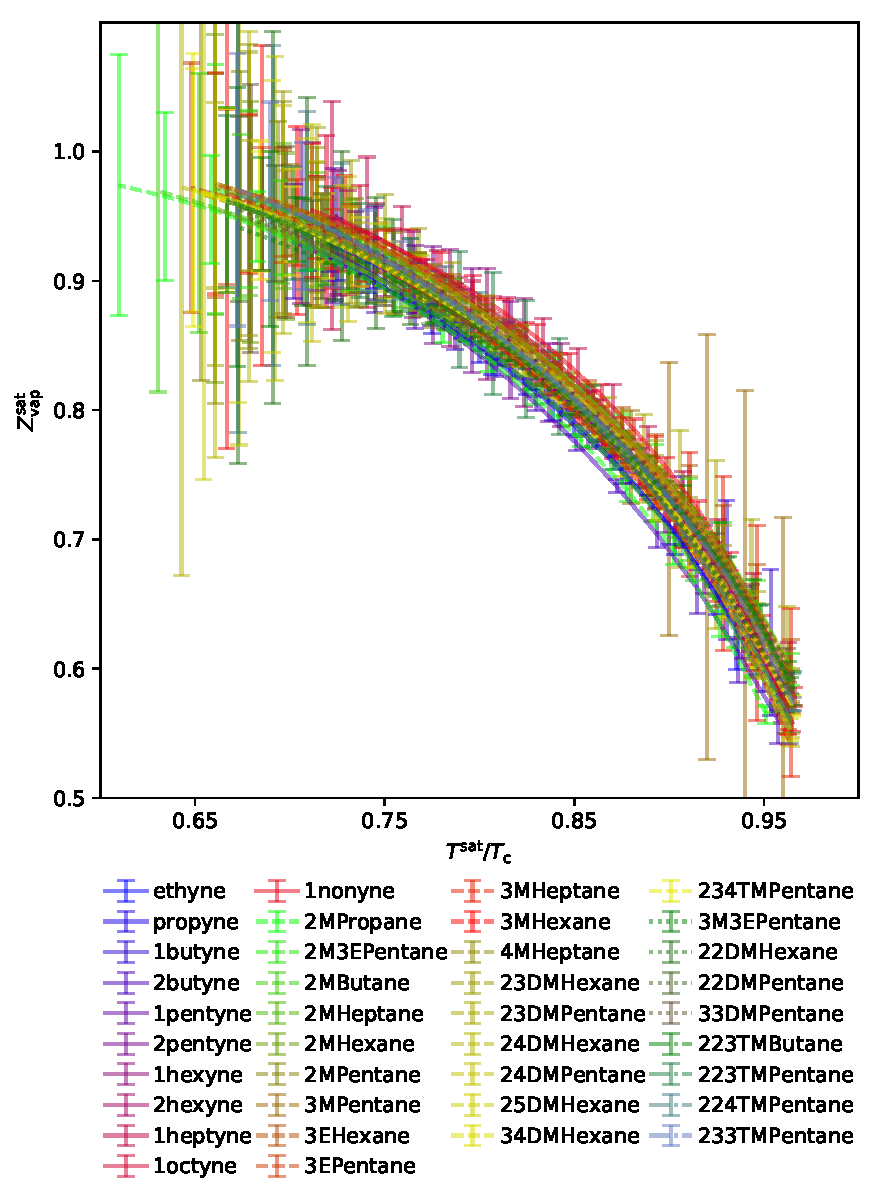
\includegraphics[width=4.8in]{Compressibility_factor_all.pdf}
	\caption{Compressibility factor in saturated vapor phase $(Z^{\rm sat}_{\rm vap})$ for all compounds simulated in Mick et al. and Soroush Barhaghi et al. Note that symmetric (normal) 95\% confidence intervals are ill-suited when $Z^{\rm sat}_{\rm vap} \approx 1$, as this assumption can result in $Z^{\rm sat}_{\rm vap} > 1$.}
	\label{SI fig:Z}
\end{figure}

\newpage
\clearpage

\subsection{Case study: Cyclohexane optimization}

\begin{figure}[htb!]
	\centering
	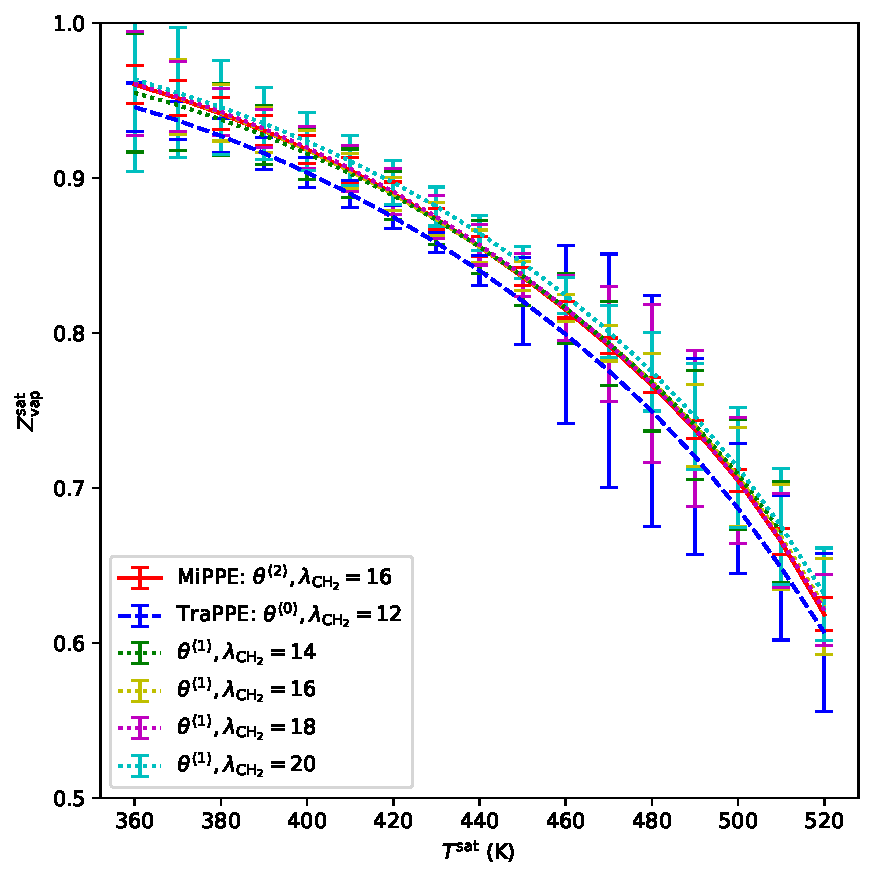
\includegraphics[width=6.4in]{Compressibility_factor_CYC6_iterations.pdf}
	\caption{Compressibility factor in saturated vapor phase $(Z^{\rm sat}_{\rm vap})$ for iterations of cyclohexane optimization. Note that symmetric (normal) 95\% confidence intervals are ill-suited when $Z^{\rm sat}_{\rm vap} \approx 1$, as this assumption can result in $Z^{\rm sat}_{\rm vap} > 1$.}
	\label{SI fig:Z_CYC6}
\end{figure}

\newpage
\clearpage

\subsection{TAMie validation}

\begin{figure}[htb!]
	\centering
	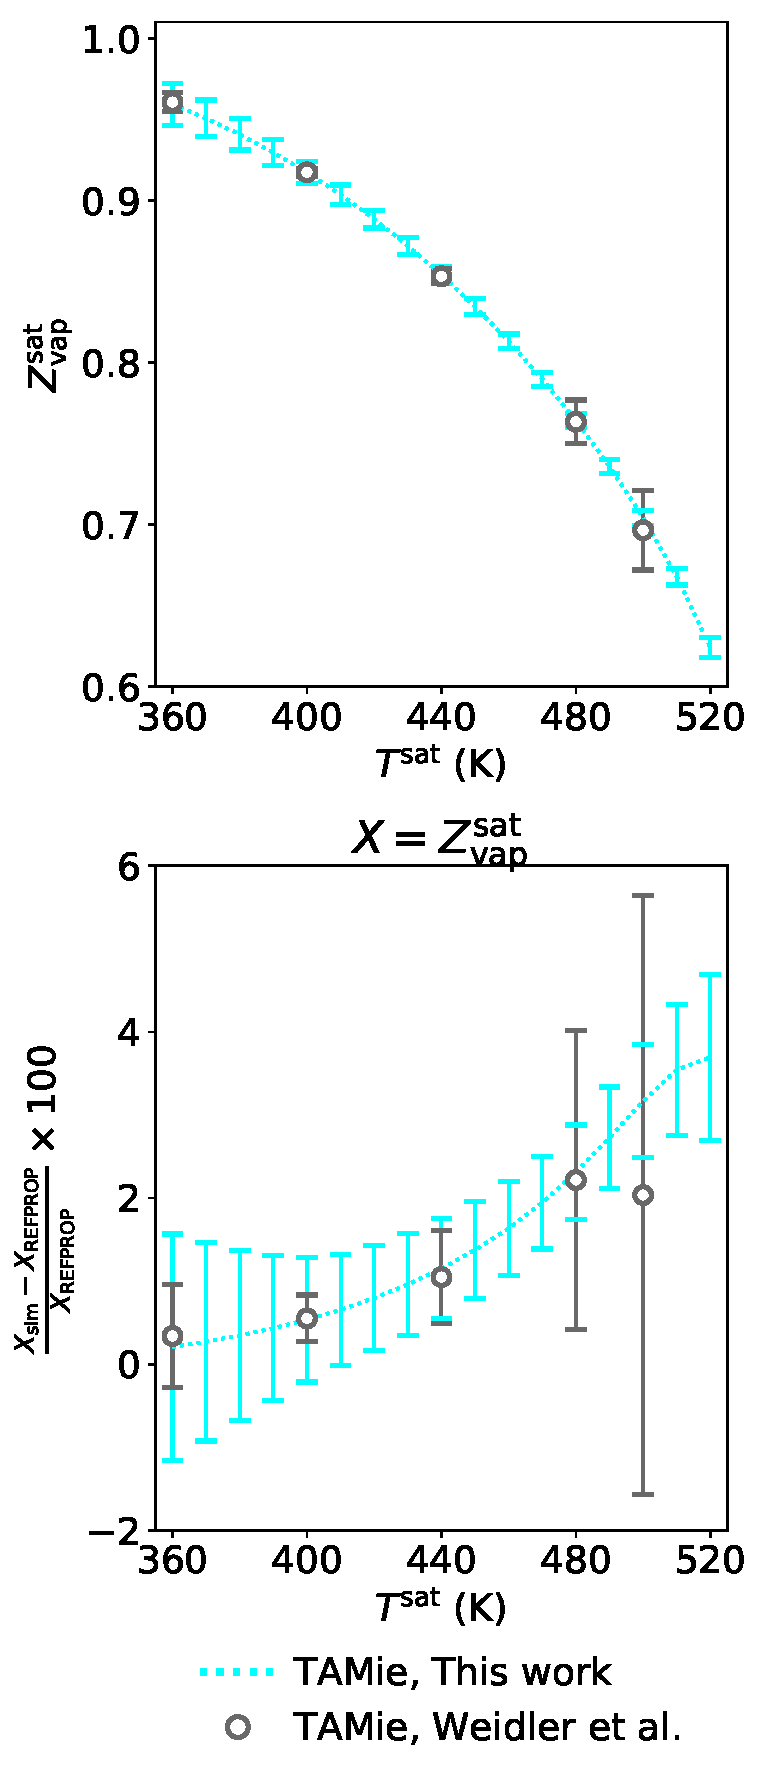
\includegraphics[width=3.0in]{Compressibility_factor_CYC6_MiPPE_TAMie.pdf}
	\caption{Comparison of compressibility factor in saturated vapor phase $(Z^{\rm sat}_{\rm vap})$ for TAMie (from this work and Weidler et al.). Simulations from this work utilized 3.5 nm box length with a 1.4 nm cut-off. Error bars apply standard propagation of error that assumes independence of $\rho_{\rm vap}^{\rm sat}$ and $P_{\rm vap}^{\rm sat}$.}
	\label{SI fig:Z_CYC6_TAMie}
\end{figure}

\newpage
\clearpage

\section{Tabulated phase equilibria for validation of GCMC-MBAR} \label{SI sec: Tabulated MBAR results}

\subsection{Branched alkanes}

\begin{table}[htb!]
	\caption{GCMC-MBAR results for 2-methylpropane with the MiPPE-SL force field. Subscripts correspond to the 95\% confidence interval computed with bootstrap re-sampling.}
	\begin{center}
		\begin{tabular}{|c|c|c|c|c|c|}
			\hline
			$T^{\rm sat}$ (K) & $\rho_{\rm liq}^{\rm sat}$ (kg/m$^3$) & $\rho_{\rm vap}^{\rm sat}$ (kg/m$^3$) & $P_{\rm vap}^{\rm sat}$ (MPa) & $\Delta H_{\rm v}$ (kJ/mol) & $Z_{\rm vap}^{\rm sat}$ \\ \hline
			390 & $388.8_{8.4}$ & $87.1_{1.6}$ & $2.742_{0.026}$ & $9.76_{0.34}$ & $0.56_{0.01}$ \\
			380 & $416.6_{4.6}$ & $66.4_{1.2}$ & $2.292_{0.026}$ & $11.69_{0.17}$ & $0.63_{0.01}$ \\
			370 & $439.7_{1.3}$ & $51.95_{0.77}$ & $1.903_{0.025}$ & $13.219_{0.077}$ & $0.692_{0.011}$ \\
			360 & $459.18_{0.47}$ & $41.22_{0.53}$ & $1.566_{0.023}$ & $14.442_{0.060}$ & $0.74_{0.01}$ \\
			350 & $476.39_{0.48}$ & $32.82_{0.53}$ & $1.276_{0.019}$ & $15.485_{0.049}$ & $0.78_{0.01}$ \\
			340 & $492.09_{0.59}$ & $26.09_{0.54}$ & $1.028_{0.015}$ & $16.404_{0.052}$ & $0.81_{0.01}$ \\
			330 & $506.65_{0.67}$ & $20.62_{0.48}$ & $0.817_{0.011}$ & $17.227_{0.055}$ & $0.84_{0.01}$ \\
			320 & $520.48_{0.53}$ & $16.16_{0.39}$ & $0.6403_{0.0069}$ & $17.980_{0.058}$ & $0.865_{0.013}$ \\
			310 & $533.93_{0.54}$ & $12.53_{0.27}$ & $0.4935_{0.0043}$ & $18.686_{0.062}$ & $0.889_{0.015}$ \\
			300 & $546.58_{0.63}$ & $9.57_{0.17}$ & $0.3733_{0.0032}$ & $19.332_{0.062}$ & $0.909_{0.016}$ \\
			290 & $558.46_{0.48}$ & $7.19_{0.12}$ & $0.2765_{0.0030}$ & $19.925_{0.061}$ & $0.927_{0.019}$ \\
			280 & $570.30_{0.67}$ & $5.300_{0.094}$ & $0.2000_{0.0032}$ & $20.498_{0.077}$ & $0.942_{0.027}$ \\
			270 & $582.5_{1.0}$ & $3.815_{0.083}$ & $0.1408_{0.0037}$ & $21.07_{0.11}$ & $0.955_{0.042}$ \\
			260 & $593.47_{0.60}$ & $2.672_{0.071}$ & $0.0959_{0.0043}$ & $21.57_{0.14}$ & $0.965_{0.065}$ \\
			250 & $603.0_{1.0}$ & $1.815_{0.057}$ & $0.0632_{0.0048}$ & $22.01_{0.22}$ & $0.97_{0.10}$ \\
			\hline
		\end{tabular}
	\end{center}
\end{table}

\begin{table}[htb!]
	\caption{GCMC-MBAR results for 2-methylbutane with the MiPPE-SL force field. Subscripts correspond to the 95\% confidence interval computed with bootstrap re-sampling.}
	\begin{center}
		\begin{tabular}{|c|c|c|c|c|c|}
			\hline
			$T^{\rm sat}$ (K) & $\rho_{\rm liq}^{\rm sat}$ (kg/m$^3$) & $\rho_{\rm vap}^{\rm sat}$ (kg/m$^3$) & $P_{\rm vap}^{\rm sat}$ (MPa) & $\Delta H_{\rm v}$ (kJ/mol) & $Z_{\rm vap}^{\rm sat}$ \\ \hline
			440 & $399.8_{3.5}$ & $86.6_{2.1}$ & $2.528_{0.020}$ & $11.558_{0.090}$ & $0.58_{0.01}$ \\
			430 & $426.9_{2.6}$ & $68.9_{1.7}$ & $2.149_{0.011}$ & $13.44_{0.11}$ & $0.629_{0.012}$ \\
			420 & $449.4_{1.4}$ & $55.1_{1.2}$ & $1.8149_{0.0059}$ & $15.07_{0.11}$ & $0.680_{0.012}$ \\
			410 & $468.58_{0.70}$ & $44.49_{0.66}$ & $1.5225_{0.0039}$ & $16.438_{0.094}$ & $0.724_{0.010}$ \\
			400 & $485.59_{0.52}$ & $36.12_{0.31}$ & $1.2671_{0.0037}$ & $17.615_{0.066}$ & $0.76_{0.01}$ \\
			390 & $501.08_{0.68}$ & $29.33_{0.15}$ & $1.0450_{0.0036}$ & $18.654_{0.048}$ & $0.79_{0.01}$ \\
			380 & $515.41_{0.89}$ & $23.73_{0.12}$ & $0.8532_{0.0034}$ & $19.590_{0.055}$ & $0.82_{0.01}$ \\
			370 & $528.88_{0.98}$ & $19.09_{0.11}$ & $0.6887_{0.0031}$ & $20.447_{0.064}$ & $0.85_{0.01}$ \\
			360 & $541.7_{1.0}$ & $15.230_{0.098}$ & $0.5489_{0.0029}$ & $21.238_{0.067}$ & $0.87_{0.01}$ \\
			350 & $553.9_{1.1}$ & $12.03_{0.10}$ & $0.4315_{0.0028}$ & $21.976_{0.071}$ & $0.889_{0.010}$ \\
			340 & $565.8_{1.3}$ & $9.40_{0.11}$ & $0.3341_{0.0029}$ & $22.678_{0.085}$ & $0.907_{0.016}$ \\
			330 & $577.7_{1.7}$ & $7.24_{0.12}$ & $0.2541_{0.0033}$ & $23.35_{0.12}$ & $0.923_{0.025}$ \\
			320 & $588.9_{1.7}$ & $5.48_{0.14}$ & $0.1896_{0.0039}$ & $23.98_{0.16}$ & $0.938_{0.040}$ \\
			310 & $598.9_{1.2}$ & $4.08_{0.14}$ & $0.1385_{0.0047}$ & $24.53_{0.20}$ & $0.950_{0.064}$ \\
			300 & $608.6_{1.2}$ & $2.98_{0.14}$ & $0.0988_{0.0055}$ & $25.06_{0.28}$ & $0.960_{0.10}$ \\
			290 & $618.9_{1.3}$ & $2.12_{0.13}$ & $0.0686_{0.0064}$ & $25.61_{0.41}$ & $0.97_{0.16}$ \\
			\hline
		\end{tabular}
	\end{center}
\end{table}

\begin{table}[htb!]
	\caption{GCMC-MBAR results for 2-methylpentane with the MiPPE-SL force field. Subscripts correspond to the 95\% confidence interval computed with bootstrap re-sampling.}
	\begin{center}
		\begin{tabular}{|c|c|c|c|c|c|}
			\hline
			$T^{\rm sat}$ (K) & $\rho_{\rm liq}^{\rm sat}$ (kg/m$^3$) & $\rho_{\rm vap}^{\rm sat}$ (kg/m$^3$) & $P_{\rm vap}^{\rm sat}$ (MPa) & $\Delta H_{\rm v}$ (kJ/mol) & $Z_{\rm vap}^{\rm sat}$ \\ \hline
			470 & $422.20_{0.56}$ & $76.7_{1.5}$ & $2.068_{0.017}$ & $14.14_{0.11}$ & $0.59_{0.01}$ \\
			460 & $444.71_{0.79}$ & $61.2_{1.2}$ & $1.761_{0.013}$ & $16.06_{0.12}$ & $0.65_{0.01}$ \\
			450 & $464.38_{0.87}$ & $49.31_{0.88}$ & $1.4918_{0.0096}$ & $17.71_{0.11}$ & $0.70_{0.01}$ \\
			440 & $481.69_{0.77}$ & $40.17_{0.64}$ & $1.2557_{0.0068}$ & $19.106_{0.090}$ & $0.74_{0.01}$ \\
			430 & $497.34_{0.70}$ & $32.86_{0.47}$ & $1.0491_{0.0045}$ & $20.318_{0.074}$ & $0.77_{0.01}$ \\
			420 & $511.89_{0.78}$ & $26.86_{0.36}$ & $0.8690_{0.0027}$ & $21.408_{0.068}$ & $0.80_{0.01}$ \\
			410 & $525.69_{0.84}$ & $21.87_{0.29}$ & $0.7130_{0.0017}$ & $22.412_{0.069}$ & $0.824_{0.011}$ \\
			400 & $538.82_{0.88}$ & $17.70_{0.25}$ & $0.5788_{0.0020}$ & $23.344_{0.069}$ & $0.848_{0.014}$ \\
			390 & $551.23_{0.87}$ & $14.21_{0.22}$ & $0.4645_{0.0031}$ & $24.207_{0.075}$ & $0.869_{0.018}$ \\
			380 & $562.89_{0.80}$ & $11.30_{0.19}$ & $0.3681_{0.0042}$ & $25.004_{0.096}$ & $0.888_{0.024}$ \\
			370 & $573.96_{0.88}$ & $8.90_{0.16}$ & $0.2878_{0.0051}$ & $25.75_{0.14}$ & $0.906_{0.032}$ \\
			360 & $584.8_{1.1}$ & $6.92_{0.14}$ & $0.2215_{0.0059}$ & $26.46_{0.18}$ & $0.922_{0.042}$ \\
			350 & $595.6_{1.2}$ & $5.31_{0.12}$ & $0.1677_{0.0065}$ & $27.15_{0.22}$ & $0.935_{0.056}$ \\
			340 & $606.3_{1.2}$ & $4.01_{0.10}$ & $0.1245_{0.0070}$ & $27.83_{0.27}$ & $0.947_{0.076}$ \\
			330 & $616.4_{1.0}$ & $2.969_{0.085}$ & $0.0906_{0.0074}$ & $28.45_{0.32}$ & $0.96_{0.10}$ \\
			320 & $625.82_{0.57}$ & $2.156_{0.068}$ & $0.0644_{0.0078}$ & $29.04_{0.40}$ & $0.97_{0.14}$ \\
			\hline
		\end{tabular}
	\end{center}
\end{table}

\begin{table}[htb!]
	\caption{GCMC-MBAR results for 2-methylhexane with the MiPPE-SL force field. Subscripts correspond to the 95\% confidence interval computed with bootstrap re-sampling.}
	\begin{center}
		\begin{tabular}{|c|c|c|c|c|c|}
			\hline
			$T^{\rm sat}$ (K) & $\rho_{\rm liq}^{\rm sat}$ (kg/m$^3$) & $\rho_{\rm vap}^{\rm sat}$ (kg/m$^3$) & $P_{\rm vap}^{\rm sat}$ (MPa) & $\Delta H_{\rm v}$ (kJ/mol) & $Z_{\rm vap}^{\rm sat}$ \\ \hline
			510 & $406.8_{3.4}$ & $88.4_{2.0}$ & $2.092_{0.011}$ & $14.14_{0.12}$ & $0.56_{0.01}$ \\
			500 & $431.2_{2.2}$ & $70.0_{1.6}$ & $1.7989_{0.0052}$ & $16.506_{0.085}$ & $0.620_{0.013}$ \\
			490 & $452.1_{1.2}$ & $56.5_{1.0}$ & $1.5403_{0.0041}$ & $18.472_{0.088}$ & $0.671_{0.013}$ \\
			480 & $470.38_{0.73}$ & $46.30_{0.50}$ & $1.3120_{0.0056}$ & $20.092_{0.065}$ & $0.712_{0.010}$ \\
			470 & $486.88_{0.50}$ & $38.21_{0.17}$ & $1.1104_{0.0062}$ & $21.497_{0.034}$ & $0.75_{0.01}$ \\
			460 & $502.20_{0.37}$ & $31.56_{0.16}$ & $0.9327_{0.0058}$ & $22.762_{0.022}$ & $0.77_{0.01}$ \\
			450 & $516.52_{0.39}$ & $26.01_{0.17}$ & $0.7772_{0.0050}$ & $23.921_{0.024}$ & $0.80_{0.01}$ \\
			440 & $530.01_{0.34}$ & $21.34_{0.15}$ & $0.6417_{0.0043}$ & $24.994_{0.024}$ & $0.82_{0.01}$ \\
			430 & $542.86_{0.37}$ & $17.41_{0.14}$ & $0.5245_{0.0039}$ & $25.998_{0.031}$ & $0.84_{0.01}$ \\
			420 & $554.93_{0.46}$ & $14.10_{0.13}$ & $0.4241_{0.0037}$ & $26.928_{0.041}$ & $0.86_{0.01}$ \\
			410 & $566.22_{0.43}$ & $11.32_{0.14}$ & $0.3390_{0.0036}$ & $27.789_{0.046}$ & $0.881_{0.014}$ \\
			400 & $577.21_{0.43}$ & $8.99_{0.14}$ & $0.2674_{0.0037}$ & $28.610_{0.060}$ & $0.896_{0.020}$ \\
			390 & $588.02_{0.38}$ & $7.06_{0.15}$ & $0.2080_{0.0039}$ & $29.403_{0.089}$ & $0.910_{0.030}$ \\
			380 & $598.35_{0.22}$ & $5.47_{0.16}$ & $0.1593_{0.0044}$ & $30.15_{0.14}$ & $0.923_{0.044}$ \\
			370 & $608.04_{0.19}$ & $4.18_{0.16}$ & $0.1200_{0.0050}$ & $30.85_{0.20}$ & $0.935_{0.064}$ \\
			360 & $617.49_{0.27}$ & $3.14_{0.16}$ & $0.0888_{0.0057}$ & $31.52_{0.28}$ & $0.945_{0.093}$ \\
			350 & $627.22_{0.26}$ & $2.32_{0.15}$ & $0.0644_{0.0065}$ & $32.20_{0.39}$ & $0.96_{0.13}$ \\
			\hline
		\end{tabular}
	\end{center}
\end{table}

\begin{table}[htb!]
	\caption{GCMC-MBAR results for 2-methylheptane with the MiPPE-SL force field. Subscripts correspond to the 95\% confidence interval computed with bootstrap re-sampling.}
	\begin{center}
		\begin{tabular}{|c|c|c|c|c|c|}
			\hline
			$T^{\rm sat}$ (K) & $\rho_{\rm liq}^{\rm sat}$ (kg/m$^3$) & $\rho_{\rm vap}^{\rm sat}$ (kg/m$^3$) & $P_{\rm vap}^{\rm sat}$ (MPa) & $\Delta H_{\rm v}$ (kJ/mol) & $Z_{\rm vap}^{\rm sat}$ \\ \hline
			540 & $401.3_{3.7}$ & $88.7_{2.6}$ & $1.947_{0.032}$ & $15.17_{0.13}$ & $0.56_{0.01}$ \\
			530 & $426.3_{2.7}$ & $71.5_{2.6}$ & $1.683_{0.023}$ & $17.60_{0.12}$ & $0.610_{0.015}$ \\
			520 & $448.1_{1.4}$ & $58.0_{2.1}$ & $1.447_{0.015}$ & $19.75_{0.16}$ & $0.660_{0.020}$ \\
			510 & $467.12_{0.68}$ & $47.5_{1.5}$ & $1.2389_{0.0097}$ & $21.59_{0.16}$ & $0.702_{0.019}$ \\
			500 & $483.89_{0.51}$ & $39.23_{0.90}$ & $1.0545_{0.0068}$ & $23.17_{0.13}$ & $0.738_{0.016}$ \\
			490 & $499.04_{0.51}$ & $32.49_{0.54}$ & $0.8917_{0.0055}$ & $24.571_{0.096}$ & $0.770_{0.012}$ \\
			480 & $513.07_{0.62}$ & $26.88_{0.35}$ & $0.7488_{0.0048}$ & $25.842_{0.079}$ & $0.80_{0.01}$ \\
			470 & $526.33_{0.63}$ & $22.18_{0.26}$ & $0.6238_{0.0042}$ & $27.019_{0.072}$ & $0.82_{0.01}$ \\
			460 & $538.86_{0.70}$ & $18.22_{0.22}$ & $0.5151_{0.0038}$ & $28.112_{0.079}$ & $0.844_{0.010}$ \\
			450 & $550.62_{0.83}$ & $14.88_{0.19}$ & $0.4215_{0.0036}$ & $29.125_{0.091}$ & $0.865_{0.013}$ \\
			440 & $561.64_{0.82}$ & $12.07_{0.16}$ & $0.3414_{0.0037}$ & $30.06_{0.10}$ & $0.883_{0.017}$ \\
			430 & $572.07_{0.80}$ & $9.71_{0.14}$ & $0.2735_{0.0040}$ & $30.94_{0.11}$ & $0.900_{0.022}$ \\
			420 & $582.24_{0.77}$ & $7.74_{0.11}$ & $0.2165_{0.0043}$ & $31.78_{0.13}$ & $0.915_{0.028}$ \\
			410 & $592.62_{0.67}$ & $6.108_{0.092}$ & $0.1691_{0.0045}$ & $32.62_{0.14}$ & $0.927_{0.035}$ \\
			400 & $603.09_{0.65}$ & $4.758_{0.074}$ & $0.1302_{0.0047}$ & $33.44_{0.16}$ & $0.940_{0.044}$ \\
			390 & $612.67_{0.70}$ & $3.655_{0.061}$ & $0.0986_{0.0049}$ & $34.20_{0.19}$ & $0.950_{0.056}$ \\
			380 & $621.39_{0.62}$ & $2.766_{0.052}$ & $0.0734_{0.0049}$ & $34.89_{0.24}$ & $0.960_{0.071}$ \\
			370 & $630.41_{0.64}$ & $2.057_{0.045}$ & $0.0536_{0.0049}$ & $35.58_{0.31}$ & $0.967_{0.093}$ \\
			\hline
		\end{tabular}
	\end{center}
\end{table}

\begin{table}[htb!]
	\caption{GCMC-MBAR results for 3-methylpentane with the MiPPE-SL force field. Subscripts correspond to the 95\% confidence interval computed with bootstrap re-sampling.}
	\begin{center}
		\begin{tabular}{|c|c|c|c|c|c|}
			\hline
			$T^{\rm sat}$ (K) & $\rho_{\rm liq}^{\rm sat}$ (kg/m$^3$) & $\rho_{\rm vap}^{\rm sat}$ (kg/m$^3$) & $P_{\rm vap}^{\rm sat}$ (MPa) & $\Delta H_{\rm v}$ (kJ/mol) & $Z_{\rm vap}^{\rm sat}$ \\ \hline
			480 & $415.8_{1.5}$ & $84_{24}$ & $2.31_{0.24}$ & $13.7_{1.3}$ & $0.60_{0.12}$ \\
			470 & $440.0_{2.3}$ & $67_{24}$ & $1.99_{0.14}$ & $15.6_{1.7}$ & $0.65_{0.17}$ \\
			460 & $459.8_{2.5}$ & $55_{18}$ & $1.698_{0.059}$ & $17.2_{1.6}$ & $0.69_{0.16}$ \\
			450 & $477.1_{1.9}$ & $45.4_{7.6}$ & $1.443_{0.012}$ & $18.52_{0.94}$ & $0.73_{0.11}$ \\
			440 & $493.2_{1.2}$ & $37.5_{1.5}$ & $1.217_{0.014}$ & $19.74_{0.27}$ & $0.764_{0.036}$ \\
			430 & $508.9_{1.4}$ & $30.95_{0.38}$ & $1.019_{0.015}$ & $20.87_{0.11}$ & $0.794_{0.013}$ \\
			420 & $523.6_{1.1}$ & $25.42_{0.36}$ & $0.845_{0.014}$ & $21.917_{0.094}$ & $0.821_{0.016}$ \\
			410 & $536.8_{1.4}$ & $20.78_{0.32}$ & $0.695_{0.014}$ & $22.85_{0.12}$ & $0.845_{0.020}$ \\
			400 & $548.9_{1.7}$ & $16.89_{0.24}$ & $0.565_{0.013}$ & $23.69_{0.15}$ & $0.867_{0.021}$ \\
			390 & $560.5_{1.5}$ & $13.63_{0.21}$ & $0.455_{0.012}$ & $24.49_{0.13}$ & $0.887_{0.018}$ \\
			380 & $571.8_{1.2}$ & $10.88_{0.20}$ & $0.361_{0.010}$ & $25.250_{0.099}$ & $0.905_{0.016}$ \\
			370 & $582.3_{1.1}$ & $8.59_{0.18}$ & $0.2829_{0.0089}$ & $25.950_{0.093}$ & $0.922_{0.018}$ \\
			360 & $593.0_{1.1}$ & $6.70_{0.16}$ & $0.2185_{0.0077}$ & $26.64_{0.12}$ & $0.939_{0.024}$ \\
			350 & $603.8_{1.0}$ & $5.15_{0.14}$ & $0.1661_{0.0067}$ & $27.33_{0.14}$ & $0.955_{0.035}$ \\
			\hline
		\end{tabular}
	\end{center}
\end{table}

\begin{table}[htb!]
	\caption{GCMC-MBAR results for 3-methylhexane with the MiPPE-SL force field. Subscripts correspond to the 95\% confidence interval computed with bootstrap re-sampling.}
	\begin{center}
		\begin{tabular}{|c|c|c|c|c|c|}
			\hline
			$T^{\rm sat}$ (K) & $\rho_{\rm liq}^{\rm sat}$ (kg/m$^3$) & $\rho_{\rm vap}^{\rm sat}$ (kg/m$^3$) & $P_{\rm vap}^{\rm sat}$ (MPa) & $\Delta H_{\rm v}$ (kJ/mol) & $Z_{\rm vap}^{\rm sat}$ \\ \hline
			520 & $398.4_{4.6}$ & $98.1_{1.2}$ & $2.307_{0.018}$ & $13.25_{0.29}$ & $0.55_{0.01}$ \\
			510 & $426.2_{3.4}$ & $77.3_{1.3}$ & $1.996_{0.015}$ & $15.86_{0.21}$ & $0.61_{0.01}$ \\
			500 & $449.0_{1.8}$ & $62.6_{1.1}$ & $1.720_{0.012}$ & $17.92_{0.14}$ & $0.66_{0.01}$ \\
			490 & $467.85_{0.87}$ & $51.64_{0.76}$ & $1.474_{0.011}$ & $19.56_{0.10}$ & $0.70_{0.01}$ \\
			480 & $484.12_{0.71}$ & $42.82_{0.51}$ & $1.2562_{0.0093}$ & $20.963_{0.074}$ & $0.74_{0.01}$ \\
			470 & $498.93_{0.76}$ & $35.54_{0.44}$ & $1.0638_{0.0075}$ & $22.215_{0.069}$ & $0.77_{0.01}$ \\
			460 & $512.9_{1.0}$ & $29.46_{0.42}$ & $0.8944_{0.0056}$ & $23.366_{0.088}$ & $0.80_{0.01}$ \\
			450 & $526.2_{1.3}$ & $24.34_{0.36}$ & $0.7463_{0.0040}$ & $24.442_{0.093}$ & $0.82_{0.01}$ \\
			440 & $539.09_{0.79}$ & $20.03_{0.26}$ & $0.6171_{0.0029}$ & $25.454_{0.048}$ & $0.84_{0.01}$ \\
			430 & $551.25_{0.90}$ & $16.38_{0.15}$ & $0.5055_{0.0025}$ & $26.397_{0.089}$ & $0.86_{0.01}$ \\
			420 & $563.0_{1.6}$ & $13.302_{0.087}$ & $0.4097_{0.0025}$ & $27.29_{0.16}$ & $0.88_{0.01}$ \\
			410 & $574.5_{1.4}$ & $10.70_{0.12}$ & $0.3283_{0.0024}$ & $28.15_{0.18}$ & $0.90_{0.01}$ \\
			400 & $585.3_{1.3}$ & $8.53_{0.18}$ & $0.2598_{0.0021}$ & $28.96_{0.19}$ & $0.918_{0.019}$ \\
			390 & $595.7_{2.4}$ & $6.72_{0.26}$ & $0.2028_{0.0021}$ & $29.72_{0.30}$ & $0.933_{0.039}$ \\
			380 & $605.9_{2.8}$ & $5.23_{0.33}$ & $0.1560_{0.0032}$ & $30.45_{0.41}$ & $0.947_{0.073}$ \\
			370 & $615.4_{1.3}$ & $4.01_{0.38}$ & $0.1181_{0.0053}$ & $31.13_{0.47}$ & $0.96_{0.12}$ \\
			360 & $624.92_{0.55}$ & $3.04_{0.40}$ & $0.0878_{0.0081}$ & $31.78_{0.63}$ & $0.97_{0.20}$ \\
			\hline
		\end{tabular}
	\end{center}
\end{table}

\begin{table}[htb!]
	\caption{GCMC-MBAR results for 3-methylheptane with the MiPPE-SL force field. Subscripts correspond to the 95\% confidence interval computed with bootstrap re-sampling.}
	\begin{center}
		\begin{tabular}{|c|c|c|c|c|c|}
			\hline
			$T^{\rm sat}$ (K) & $\rho_{\rm liq}^{\rm sat}$ (kg/m$^3$) & $\rho_{\rm vap}^{\rm sat}$ (kg/m$^3$) & $P_{\rm vap}^{\rm sat}$ (MPa) & $\Delta H_{\rm v}$ (kJ/mol) & $Z_{\rm vap}^{\rm sat}$ \\ \hline
			540 & $417.2_{1.2}$ & $83_{12}$ & $1.890_{0.063}$ & $16.23_{0.82}$ & $0.582_{0.065}$ \\
			530 & $440.3_{1.2}$ & $66.7_{9.0}$ & $1.634_{0.033}$ & $18.58_{0.89}$ & $0.635_{0.076}$ \\
			520 & $460.5_{1.2}$ & $54.5_{5.6}$ & $1.407_{0.012}$ & $20.58_{0.75}$ & $0.681_{0.067}$ \\
			510 & $478.1_{1.2}$ & $45.1_{2.8}$ & $1.2045_{0.0059}$ & $22.26_{0.50}$ & $0.719_{0.048}$ \\
			500 & $494.01_{0.92}$ & $37.5_{1.1}$ & $1.0252_{0.0098}$ & $23.73_{0.26}$ & $0.752_{0.028}$ \\
			490 & $508.73_{0.65}$ & $31.13_{0.27}$ & $0.867_{0.011}$ & $25.068_{0.10}$ & $0.781_{0.013}$ \\
			480 & $522.52_{0.51}$ & $25.80_{0.29}$ & $0.728_{0.010}$ & $26.295_{0.066}$ & $0.81_{0.01}$ \\
			470 & $535.46_{0.54}$ & $21.31_{0.32}$ & $0.6061_{0.0088}$ & $27.431_{0.087}$ & $0.83_{0.01}$ \\
			460 & $547.59_{0.69}$ & $17.52_{0.28}$ & $0.5005_{0.0075}$ & $28.484_{0.098}$ & $0.85_{0.01}$ \\
			450 & $559.13_{0.85}$ & $14.31_{0.24}$ & $0.4094_{0.0063}$ & $29.47_{0.11}$ & $0.87_{0.01}$ \\
			440 & $570.31_{0.88}$ & $11.61_{0.22}$ & $0.3315_{0.0051}$ & $30.41_{0.11}$ & $0.89_{0.01}$ \\
			430 & $581.03_{0.75}$ & $9.34_{0.20}$ & $0.2656_{0.0041}$ & $31.30_{0.11}$ & $0.91_{0.01}$ \\
			420 & $591.11_{0.65}$ & $7.44_{0.18}$ & $0.2102_{0.0031}$ & $32.12_{0.12}$ & $0.924_{0.015}$ \\
			410 & $600.65_{0.78}$ & $5.87_{0.16}$ & $0.1642_{0.0025}$ & $32.89_{0.15}$ & $0.937_{0.022}$ \\
			400 & $610.1_{1.1}$ & $4.58_{0.14}$ & $0.1265_{0.0021}$ & $33.65_{0.20}$ & $0.949_{0.032}$ \\
			390 & $620.1_{1.3}$ & $3.52_{0.12}$ & $0.0959_{0.0022}$ & $34.43_{0.24}$ & $0.959_{0.044}$ \\
			380 & $630.35_{0.84}$ & $2.67_{0.10}$ & $0.0714_{0.0025}$ & $35.23_{0.26}$ & $0.967_{0.062}$ \\
			370 & $640.62_{0.56}$ & $1.986_{0.080}$ & $0.0522_{0.0029}$ & $36.01_{0.30}$ & $0.975_{0.085}$ \\
			\hline
		\end{tabular}
	\end{center}
\end{table}

\begin{table}[htb!]
	\caption{GCMC-MBAR results for 3-ethylpentane with the MiPPE-SL force field. Subscripts correspond to the 95\% confidence interval computed with bootstrap re-sampling.}
	\begin{center}
		\begin{tabular}{|c|c|c|c|c|c|}
			\hline
			$T^{\rm sat}$ (K) & $\rho_{\rm liq}^{\rm sat}$ (kg/m$^3$) & $\rho_{\rm vap}^{\rm sat}$ (kg/m$^3$) & $P_{\rm vap}^{\rm sat}$ (MPa) & $\Delta H_{\rm v}$ (kJ/mol) & $Z_{\rm vap}^{\rm sat}$ \\ \hline
			520 & $405.9_{2.5}$ & $92.5_{3.7}$ & $2.279_{0.020}$ & $13.93_{0.27}$ & $0.571_{0.018}$ \\
			510 & $433.2_{1.4}$ & $75.3_{2.9}$ & $1.975_{0.011}$ & $16.14_{0.27}$ & $0.620_{0.021}$ \\
			500 & $456.01_{0.97}$ & $61.6_{1.8}$ & $1.7031_{0.0070}$ & $18.08_{0.24}$ & $0.667_{0.019}$ \\
			490 & $474.95_{0.93}$ & $50.83_{0.86}$ & $1.4607_{0.0069}$ & $19.70_{0.17}$ & $0.707_{0.013}$ \\
			480 & $491.46_{0.83}$ & $42.20_{0.30}$ & $1.2454_{0.0072}$ & $21.10_{0.11}$ & $0.74_{0.01}$ \\
			470 & $506.63_{0.68}$ & $35.08_{0.18}$ & $1.0550_{0.0067}$ & $22.354_{0.060}$ & $0.77_{0.01}$ \\
			460 & $521.02_{0.50}$ & $29.12_{0.22}$ & $0.8870_{0.0058}$ & $23.514_{0.046}$ & $0.80_{0.01}$ \\
			450 & $534.61_{0.44}$ & $24.08_{0.23}$ & $0.7398_{0.0048}$ & $24.589_{0.057}$ & $0.82_{0.01}$ \\
			440 & $547.23_{0.42}$ & $19.82_{0.21}$ & $0.6115_{0.0037}$ & $25.575_{0.058}$ & $0.85_{0.01}$ \\
			430 & $559.10_{0.45}$ & $16.21_{0.17}$ & $0.5007_{0.0028}$ & $26.491_{0.043}$ & $0.87_{0.01}$ \\
			420 & $570.66_{0.61}$ & $13.16_{0.11}$ & $0.4058_{0.0023}$ & $27.365_{0.031}$ & $0.88_{0.01}$ \\
			410 & $582.02_{0.53}$ & $10.587_{0.082}$ & $0.3251_{0.0022}$ & $28.205_{0.034}$ & $0.90_{0.01}$ \\
			400 & $592.79_{0.41}$ & $8.438_{0.086}$ & $0.2572_{0.0023}$ & $28.992_{0.054}$ & $0.918_{0.015}$ \\
			390 & $602.92_{0.51}$ & $6.653_{0.098}$ & $0.2007_{0.0026}$ & $29.724_{0.089}$ & $0.932_{0.023}$ \\
			380 & $612.81_{0.53}$ & $5.18_{0.10}$ & $0.1544_{0.0030}$ & $30.43_{0.12}$ & $0.945_{0.033}$ \\
			370 & $622.47_{0.37}$ & $3.982_{0.097}$ & $0.1168_{0.0035}$ & $31.10_{0.15}$ & $0.956_{0.048}$ \\
			360 & $631.88_{0.27}$ & $3.012_{0.090}$ & $0.0868_{0.0040}$ & $31.75_{0.21}$ & $0.965_{0.068}$ \\
			350 & $641.27_{0.30}$ & $2.238_{0.081}$ & $0.0632_{0.0044}$ & $32.39_{0.29}$ & $0.972_{0.097}$ \\
			\hline
		\end{tabular}
	\end{center}
\end{table}

\begin{table}[htb!]
	\caption{GCMC-MBAR results for 3-ethylhexane with the MiPPE-SL force field. Subscripts correspond to the 95\% confidence interval computed with bootstrap re-sampling.}
	\begin{center}
		\begin{tabular}{|c|c|c|c|c|c|}
			\hline
			$T^{\rm sat}$ (K) & $\rho_{\rm liq}^{\rm sat}$ (kg/m$^3$) & $\rho_{\rm vap}^{\rm sat}$ (kg/m$^3$) & $P_{\rm vap}^{\rm sat}$ (MPa) & $\Delta H_{\rm v}$ (kJ/mol) & $Z_{\rm vap}^{\rm sat}$ \\ \hline
			540 & $425.4_{1.8}$ & $79.4_{4.9}$ & $1.866_{0.043}$ & $16.85_{0.40}$ & $0.598_{0.025}$ \\
			530 & $449.1_{1.4}$ & $64.7_{4.4}$ & $1.614_{0.029}$ & $19.05_{0.45}$ & $0.647_{0.034}$ \\
			520 & $468.9_{1.0}$ & $53.1_{3.2}$ & $1.390_{0.017}$ & $20.94_{0.42}$ & $0.691_{0.035}$ \\
			510 & $486.13_{0.88}$ & $44.0_{2.0}$ & $1.1907_{0.0092}$ & $22.56_{0.34}$ & $0.728_{0.029}$ \\
			500 & $501.71_{0.68}$ & $36.6_{1.1}$ & $1.0141_{0.0047}$ & $23.99_{0.23}$ & $0.760_{0.021}$ \\
			490 & $516.13_{0.49}$ & $30.49_{0.54}$ & $0.8581_{0.0029}$ & $25.28_{0.14}$ & $0.789_{0.013}$ \\
			480 & $529.64_{0.54}$ & $25.32_{0.27}$ & $0.7207_{0.0024}$ & $26.475_{0.089}$ & $0.81_{0.01}$ \\
			470 & $542.43_{0.64}$ & $20.95_{0.17}$ & $0.6006_{0.0021}$ & $27.583_{0.069}$ & $0.84_{0.01}$ \\
			460 & $554.62_{0.65}$ & $17.25_{0.13}$ & $0.4962_{0.0019}$ & $28.624_{0.065}$ & $0.86_{0.01}$ \\
			450 & $566.22_{0.66}$ & $14.11_{0.11}$ & $0.4063_{0.0017}$ & $29.600_{0.066}$ & $0.88_{0.01}$ \\
			440 & $577.33_{0.67}$ & $11.466_{0.088}$ & $0.3292_{0.0016}$ & $30.521_{0.065}$ & $0.90_{0.01}$ \\
			430 & $588.23_{0.68}$ & $9.237_{0.067}$ & $0.2638_{0.0016}$ & $31.409_{0.064}$ & $0.91_{0.01}$ \\
			420 & $598.94_{0.67}$ & $7.369_{0.055}$ & $0.2088_{0.0018}$ & $32.268_{0.063}$ & $0.927_{0.013}$ \\
			410 & $609.11_{0.53}$ & $5.815_{0.055}$ & $0.1630_{0.0019}$ & $33.074_{0.060}$ & $0.939_{0.019}$ \\
			400 & $618.75_{0.46}$ & $4.534_{0.059}$ & $0.1255_{0.0022}$ & $33.831_{0.070}$ & $0.950_{0.028}$ \\
			390 & $628.18_{0.46}$ & $3.487_{0.060}$ & $0.0950_{0.0025}$ & $34.56_{0.10}$ & $0.960_{0.041}$ \\
			380 & $637.85_{0.36}$ & $2.641_{0.057}$ & $0.0707_{0.0028}$ & $35.31_{0.15}$ & $0.968_{0.060}$ \\
			370 & $647.74_{0.30}$ & $1.965_{0.051}$ & $0.0515_{0.0031}$ & $36.05_{0.23}$ & $0.974_{0.087}$ \\
			\hline
		\end{tabular}
	\end{center}
\end{table}

\begin{table}[htb!]
	\caption{GCMC-MBAR results for 4-methylheptane with the MiPPE-SL force field. Subscripts correspond to the 95\% confidence interval computed with bootstrap re-sampling.}
	\begin{center}
		\begin{tabular}{|c|c|c|c|c|c|}
			\hline
			$T^{\rm sat}$ (K) & $\rho_{\rm liq}^{\rm sat}$ (kg/m$^3$) & $\rho_{\rm vap}^{\rm sat}$ (kg/m$^3$) & $P_{\rm vap}^{\rm sat}$ (MPa) & $\Delta H_{\rm v}$ (kJ/mol) & $Z_{\rm vap}^{\rm sat}$ \\ \hline
			540 & $418.9_{1.9}$ & $80.1_{1.6}$ & $1.858_{0.017}$ & $16.62_{0.17}$ & $0.59_{0.01}$ \\
			530 & $442.2_{1.4}$ & $65.0_{1.3}$ & $1.606_{0.015}$ & $18.87_{0.15}$ & $0.640_{0.010}$ \\
			520 & $462.3_{1.1}$ & $53.3_{1.1}$ & $1.382_{0.013}$ & $20.81_{0.15}$ & $0.685_{0.011}$ \\
			510 & $479.9_{1.1}$ & $44.10_{0.88}$ & $1.183_{0.010}$ & $22.48_{0.16}$ & $0.722_{0.010}$ \\
			500 & $495.8_{1.0}$ & $36.63_{0.73}$ & $1.0060_{0.0083}$ & $23.95_{0.16}$ & $0.755_{0.011}$ \\
			490 & $510.3_{1.0}$ & $30.43_{0.61}$ & $0.8501_{0.0062}$ & $25.28_{0.16}$ & $0.783_{0.011}$ \\
			480 & $523.91_{0.96}$ & $25.22_{0.47}$ & $0.7132_{0.0044}$ & $26.49_{0.15}$ & $0.809_{0.011}$ \\
			470 & $536.77_{0.78}$ & $20.83_{0.32}$ & $0.5936_{0.0029}$ & $27.62_{0.11}$ & $0.83_{0.01}$ \\
			460 & $548.98_{0.49}$ & $17.12_{0.19}$ & $0.4897_{0.0020}$ & $28.679_{0.071}$ & $0.85_{0.01}$ \\
			450 & $560.48_{0.39}$ & $13.982_{0.094}$ & $0.4002_{0.0014}$ & $29.660_{0.044}$ & $0.87_{0.01}$ \\
			440 & $571.22_{0.45}$ & $11.338_{0.062}$ & $0.3238_{0.0012}$ & $30.567_{0.048}$ & $0.89_{0.01}$ \\
			430 & $581.42_{0.48}$ & $9.118_{0.092}$ & $0.2591_{0.0013}$ & $31.419_{0.060}$ & $0.908_{0.012}$ \\
			420 & $591.67_{0.57}$ & $7.26_{0.12}$ & $0.2049_{0.0018}$ & $32.257_{0.078}$ & $0.923_{0.023}$ \\
			410 & $602.13_{0.53}$ & $5.72_{0.14}$ & $0.1598_{0.0025}$ & $33.10_{0.12}$ & $0.936_{0.037}$ \\
			400 & $612.18_{0.47}$ & $4.45_{0.14}$ & $0.1228_{0.0033}$ & $33.90_{0.18}$ & $0.947_{0.056}$ \\
			390 & $621.73_{0.54}$ & $3.42_{0.14}$ & $0.0928_{0.0042}$ & $34.65_{0.25}$ & $0.957_{0.082}$ \\
			380 & $631.63_{0.45}$ & $2.58_{0.12}$ & $0.0690_{0.0050}$ & $35.41_{0.37}$ & $0.97_{0.12}$ \\
			370 & $641.49_{0.32}$ & $1.92_{0.11}$ & $0.0502_{0.0057}$ & $36.15_{0.52}$ & $0.97_{0.17}$ \\
			\hline
		\end{tabular}
	\end{center}
\end{table}

\begin{table}[htb!]
	\caption{GCMC-MBAR results for 2,3-dimethylbutane with the MiPPE-SL force field. Subscripts correspond to the 95\% confidence interval computed with bootstrap re-sampling.}
	\begin{center}
		\begin{tabular}{|c|c|c|c|c|c|}
			\hline
			$T^{\rm sat}$ (K) & $\rho_{\rm liq}^{\rm sat}$ (kg/m$^3$) & $\rho_{\rm vap}^{\rm sat}$ (kg/m$^3$) & $P_{\rm vap}^{\rm sat}$ (MPa) & $\Delta H_{\rm v}$ (kJ/mol) & $Z_{\rm vap}^{\rm sat}$ \\ \hline
			480 & $411.7_{1.1}$ & $88.4_{2.2}$ & $2.369_{0.027}$ & $12.87_{0.14}$ & $0.58_{0.01}$ \\
			470 & $437.1_{1.0}$ & $71.6_{2.1}$ & $2.037_{0.019}$ & $14.80_{0.17}$ & $0.627_{0.013}$ \\
			460 & $459.23_{0.86}$ & $58.1_{1.6}$ & $1.742_{0.013}$ & $16.53_{0.18}$ & $0.676_{0.015}$ \\
			450 & $478.07_{0.79}$ & $47.5_{1.1}$ & $1.4813_{0.0074}$ & $18.00_{0.16}$ & $0.718_{0.014}$ \\
			440 & $494.54_{0.81}$ & $39.07_{0.72}$ & $1.2513_{0.0041}$ & $19.26_{0.13}$ & $0.754_{0.012}$ \\
			430 & $509.51_{0.77}$ & $32.20_{0.43}$ & $1.0493_{0.0024}$ & $20.37_{0.10}$ & $0.79_{0.01}$ \\
			420 & $523.51_{0.64}$ & $26.49_{0.25}$ & $0.8726_{0.0019}$ & $21.382_{0.079}$ & $0.81_{0.01}$ \\
			410 & $536.78_{0.54}$ & $21.70_{0.15}$ & $0.7189_{0.0020}$ & $22.310_{0.063}$ & $0.84_{0.01}$ \\
			400 & $549.39_{0.59}$ & $17.68_{0.10}$ & $0.5863_{0.0021}$ & $23.171_{0.060}$ & $0.86_{0.01}$ \\
			390 & $561.38_{0.73}$ & $14.296_{0.082}$ & $0.4727_{0.0023}$ & $23.971_{0.062}$ & $0.88_{0.01}$ \\
			380 & $572.70_{0.68}$ & $11.455_{0.085}$ & $0.3764_{0.0025}$ & $24.712_{0.056}$ & $0.896_{0.011}$ \\
			370 & $583.42_{0.40}$ & $9.083_{0.092}$ & $0.2957_{0.0028}$ & $25.402_{0.050}$ & $0.912_{0.016}$ \\
			360 & $593.75_{0.21}$ & $7.115_{0.095}$ & $0.2289_{0.0033}$ & $26.054_{0.064}$ & $0.926_{0.024}$ \\
			350 & $603.97_{0.20}$ & $5.497_{0.091}$ & $0.1742_{0.0037}$ & $26.686_{0.091}$ & $0.938_{0.034}$ \\
			340 & $614.11_{0.22}$ & $4.179_{0.082}$ & $0.1302_{0.0042}$ & $27.30_{0.13}$ & $0.950_{0.047}$ \\
			330 & $623.72_{0.26}$ & $3.121_{0.069}$ & $0.0953_{0.0047}$ & $27.87_{0.18}$ & $0.959_{0.066}$ \\
			320 & $632.83_{0.34}$ & $2.284_{0.057}$ & $0.0682_{0.0050}$ & $28.41_{0.25}$ & $0.968_{0.092}$ \\
			\hline
		\end{tabular}
	\end{center}
\end{table}

\begin{table}[htb!]
	\caption{GCMC-MBAR results for 2,3-dimethylhexane with the MiPPE-SL force field. Subscripts correspond to the 95\% confidence interval computed with bootstrap re-sampling.}
	\begin{center}
		\begin{tabular}{|c|c|c|c|c|c|}
			\hline
			$T^{\rm sat}$ (K) & $\rho_{\rm liq}^{\rm sat}$ (kg/m$^3$) & $\rho_{\rm vap}^{\rm sat}$ (kg/m$^3$) & $P_{\rm vap}^{\rm sat}$ (MPa) & $\Delta H_{\rm v}$ (kJ/mol) & $Z_{\rm vap}^{\rm sat}$ \\ \hline
			540 & $422.2_{1.1}$ & $84.5_{3.7}$ & $1.948_{0.048}$ & $15.98_{0.12}$ & $0.586_{0.012}$ \\
			530 & $445.87_{0.82}$ & $68.6_{3.6}$ & $1.689_{0.036}$ & $18.23_{0.22}$ & $0.638_{0.022}$ \\
			520 & $466.30_{0.66}$ & $56.3_{3.0}$ & $1.458_{0.024}$ & $20.17_{0.26}$ & $0.684_{0.027}$ \\
			510 & $484.13_{0.59}$ & $46.7_{2.1}$ & $1.253_{0.015}$ & $21.81_{0.23}$ & $0.722_{0.026}$ \\
			500 & $499.99_{0.52}$ & $39.0_{1.4}$ & $1.0703_{0.0092}$ & $23.24_{0.18}$ & $0.755_{0.022}$ \\
			490 & $514.34_{0.48}$ & $32.51_{0.80}$ & $0.9084_{0.0054}$ & $24.51_{0.13}$ & $0.783_{0.016}$ \\
			480 & $527.67_{0.54}$ & $27.08_{0.47}$ & $0.7657_{0.0032}$ & $25.677_{0.096}$ & $0.809_{0.012}$ \\
			470 & $540.41_{0.64}$ & $22.49_{0.30}$ & $0.6406_{0.0019}$ & $26.765_{0.082}$ & $0.833_{0.010}$ \\
			460 & $552.77_{0.76}$ & $18.58_{0.23}$ & $0.5313_{0.0015}$ & $27.797_{0.085}$ & $0.854_{0.011}$ \\
			450 & $564.84_{0.87}$ & $15.26_{0.22}$ & $0.4366_{0.0018}$ & $28.78_{0.11}$ & $0.874_{0.015}$ \\
			440 & $576.56_{0.95}$ & $12.43_{0.23}$ & $0.3553_{0.0025}$ & $29.73_{0.14}$ & $0.892_{0.022}$ \\
			430 & $587.55_{0.97}$ & $10.05_{0.23}$ & $0.2860_{0.0034}$ & $30.60_{0.18}$ & $0.909_{0.032}$ \\
			420 & $597.72_{0.83}$ & $8.05_{0.21}$ & $0.2274_{0.0044}$ & $31.40_{0.21}$ & $0.924_{0.043}$ \\
			410 & $607.46_{0.53}$ & $6.39_{0.18}$ & $0.1787_{0.0053}$ & $32.16_{0.22}$ & $0.937_{0.055}$ \\
			400 & $617.12_{0.48}$ & $5.01_{0.14}$ & $0.1384_{0.0061}$ & $32.90_{0.24}$ & $0.949_{0.070}$ \\
			390 & $626.72_{0.62}$ & $3.88_{0.10}$ & $0.1056_{0.0067}$ & $33.64_{0.28}$ & $0.959_{0.087}$ \\
			380 & $636.43_{0.54}$ & $2.959_{0.070}$ & $0.0792_{0.0071}$ & $34.36_{0.35}$ & $0.97_{0.11}$ \\
			370 & $646.47_{0.59}$ & $2.219_{0.049}$ & $0.0583_{0.0072}$ & $35.10_{0.46}$ & $0.98_{0.14}$ \\
			\hline
		\end{tabular}
	\end{center}
\end{table}

\begin{table}[htb!]
	\caption{GCMC-MBAR results for 2,3-dimethylpentane with the MiPPE-SL force field. Subscripts correspond to the 95\% confidence interval computed with bootstrap re-sampling.}
	\begin{center}
		\begin{tabular}{|c|c|c|c|c|c|}
			\hline
			$T^{\rm sat}$ (K) & $\rho_{\rm liq}^{\rm sat}$ (kg/m$^3$) & $\rho_{\rm vap}^{\rm sat}$ (kg/m$^3$) & $P_{\rm vap}^{\rm sat}$ (MPa) & $\Delta H_{\rm v}$ (kJ/mol) & $Z_{\rm vap}^{\rm sat}$ \\ \hline
			510 & $427.9_{1.6}$ & $81_{10}$ & $2.082_{0.091}$ & $15.20_{0.53}$ & $0.606_{0.042}$ \\
			500 & $451.7_{1.0}$ & $66.3_{9.6}$ & $1.800_{0.057}$ & $17.17_{0.70}$ & $0.654_{0.061}$ \\
			490 & $471.41_{0.86}$ & $54.7_{7.1}$ & $1.549_{0.028}$ & $18.83_{0.70}$ & $0.696_{0.065}$ \\
			480 & $488.48_{0.89}$ & $45.5_{4.0}$ & $1.3245_{0.0092}$ & $20.25_{0.54}$ & $0.731_{0.053}$ \\
			470 & $503.90_{0.73}$ & $37.9_{1.7}$ & $1.1257_{0.0050}$ & $21.50_{0.32}$ & $0.762_{0.034}$ \\
			460 & $518.28_{0.52}$ & $31.50_{0.62}$ & $0.9501_{0.0072}$ & $22.64_{0.14}$ & $0.790_{0.020}$ \\
			450 & $532.03_{0.63}$ & $26.12_{0.25}$ & $0.7956_{0.0080}$ & $23.709_{0.054}$ & $0.816_{0.013}$ \\
			440 & $545.26_{0.62}$ & $21.57_{0.18}$ & $0.6606_{0.0080}$ & $24.711_{0.037}$ & $0.839_{0.011}$ \\
			430 & $557.77_{0.54}$ & $17.70_{0.16}$ & $0.5435_{0.0075}$ & $25.646_{0.038}$ & $0.860_{0.010}$ \\
			420 & $569.33_{0.53}$ & $14.43_{0.15}$ & $0.4426_{0.0070}$ & $26.504_{0.037}$ & $0.880_{0.011}$ \\
			410 & $580.03_{0.59}$ & $11.68_{0.14}$ & $0.3565_{0.0063}$ & $27.290_{0.040}$ & $0.897_{0.012}$ \\
			400 & $590.33_{0.66}$ & $9.36_{0.13}$ & $0.2837_{0.0057}$ & $28.032_{0.047}$ & $0.913_{0.014}$ \\
			390 & $600.50_{0.61}$ & $7.43_{0.11}$ & $0.2229_{0.0052}$ & $28.747_{0.057}$ & $0.927_{0.019}$ \\
			380 & $610.33_{0.59}$ & $5.831_{0.094}$ & $0.1726_{0.0048}$ & $29.424_{0.079}$ & $0.939_{0.025}$ \\
			370 & $620.01_{0.64}$ & $4.512_{0.077}$ & $0.1315_{0.0046}$ & $30.08_{0.11}$ & $0.950_{0.036}$ \\
			360 & $630.25_{0.55}$ & $3.438_{0.066}$ & $0.0984_{0.0045}$ & $30.75_{0.14}$ & $0.959_{0.050}$ \\
			350 & $640.58_{0.49}$ & $2.572_{0.058}$ & $0.0722_{0.0046}$ & $31.42_{0.20}$ & $0.966_{0.072}$ \\
			\hline
		\end{tabular}
	\end{center}
\end{table}

\begin{table}[htb!]
	\caption{GCMC-MBAR results for 2,4-dimethylhexane with the MiPPE-SL force field. Subscripts correspond to the 95\% confidence interval computed with bootstrap re-sampling.}
	\begin{center}
		\begin{tabular}{|c|c|c|c|c|c|}
			\hline
			$T^{\rm sat}$ (K) & $\rho_{\rm liq}^{\rm sat}$ (kg/m$^3$) & $\rho_{\rm vap}^{\rm sat}$ (kg/m$^3$) & $P_{\rm vap}^{\rm sat}$ (MPa) & $\Delta H_{\rm v}$ (kJ/mol) & $Z_{\rm vap}^{\rm sat}$ \\ \hline
			540 & $406.0_{3.8}$ & $97.8_{2.1}$ & $2.090_{0.036}$ & $14.21_{0.22}$ & $0.54_{0.01}$ \\
			530 & $430.3_{3.2}$ & $78.1_{2.3}$ & $1.810_{0.028}$ & $16.71_{0.16}$ & $0.60_{0.01}$ \\
			520 & $452.1_{1.9}$ & $63.1_{2.2}$ & $1.562_{0.019}$ & $18.90_{0.15}$ & $0.654_{0.016}$ \\
			510 & $470.9_{1.1}$ & $51.8_{1.9}$ & $1.342_{0.013}$ & $20.72_{0.19}$ & $0.698_{0.020}$ \\
			500 & $487.5_{1.1}$ & $42.9_{1.4}$ & $1.1472_{0.0080}$ & $22.26_{0.19}$ & $0.734_{0.020}$ \\
			490 & $502.5_{1.2}$ & $35.72_{0.85}$ & $0.9745_{0.0054}$ & $23.60_{0.16}$ & $0.765_{0.017}$ \\
			480 & $516.3_{1.4}$ & $29.69_{0.47}$ & $0.8222_{0.0043}$ & $24.83_{0.13}$ & $0.793_{0.012}$ \\
			470 & $529.5_{1.6}$ & $24.62_{0.27}$ & $0.6886_{0.0037}$ & $25.96_{0.11}$ & $0.82_{0.01}$ \\
			460 & $542.1_{1.7}$ & $20.34_{0.18}$ & $0.5720_{0.0031}$ & $27.026_{0.098}$ & $0.84_{0.01}$ \\
			450 & $554.3_{1.8}$ & $16.71_{0.13}$ & $0.4708_{0.0026}$ & $28.031_{0.098}$ & $0.86_{0.01}$ \\
			440 & $566.1_{1.8}$ & $13.63_{0.10}$ & $0.3836_{0.0024}$ & $28.98_{0.10}$ & $0.88_{0.01}$ \\
			430 & $577.4_{1.6}$ & $11.03_{0.11}$ & $0.3092_{0.0023}$ & $29.89_{0.11}$ & $0.895_{0.010}$ \\
			420 & $588.1_{1.4}$ & $8.85_{0.15}$ & $0.2463_{0.0022}$ & $30.73_{0.13}$ & $0.910_{0.019}$ \\
			410 & $598.1_{1.1}$ & $7.02_{0.19}$ & $0.1937_{0.0024}$ & $31.51_{0.17}$ & $0.924_{0.033}$ \\
			400 & $607.97_{0.72}$ & $5.51_{0.22}$ & $0.1503_{0.0031}$ & $32.27_{0.22}$ & $0.937_{0.056}$ \\
			390 & $617.69_{0.31}$ & $4.27_{0.23}$ & $0.1148_{0.0042}$ & $33.01_{0.29}$ & $0.947_{0.088}$ \\
			380 & $627.04_{0.22}$ & $3.26_{0.22}$ & $0.0862_{0.0055}$ & $33.71_{0.42}$ & $0.96_{0.14}$ \\
			370 & $635.81_{0.19}$ & $2.45_{0.20}$ & $0.0636_{0.0068}$ & $34.36_{0.62}$ & $0.97_{0.20}$ \\
			360 & $644.04_{0.32}$ & $1.80_{0.18}$ & $0.0460_{0.0080}$ & $34.97_{0.91}$ & $0.97_{0.30}$ \\
			\hline
		\end{tabular}
	\end{center}
\end{table}

\begin{table}[htb!]
	\caption{GCMC-MBAR results for 2,4-dimethylpentane with the MiPPE-SL force field. Subscripts correspond to the 95\% confidence interval computed with bootstrap re-sampling.}
	\begin{center}
		\begin{tabular}{|c|c|c|c|c|c|}
			\hline
			$T^{\rm sat}$ (K) & $\rho_{\rm liq}^{\rm sat}$ (kg/m$^3$) & $\rho_{\rm vap}^{\rm sat}$ (kg/m$^3$) & $P_{\rm vap}^{\rm sat}$ (MPa) & $\Delta H_{\rm v}$ (kJ/mol) & $Z_{\rm vap}^{\rm sat}$ \\ \hline
			500 & $420.0_{1.7}$ & $81.9_{2.0}$ & $2.003_{0.018}$ & $14.77_{0.12}$ & $0.590_{0.011}$ \\
			490 & $443.0_{1.0}$ & $65.6_{1.4}$ & $1.722_{0.014}$ & $16.87_{0.12}$ & $0.646_{0.011}$ \\
			480 & $462.83_{0.68}$ & $53.40_{0.95}$ & $1.473_{0.011}$ & $18.632_{0.099}$ & $0.69_{0.01}$ \\
			470 & $480.50_{0.59}$ & $43.96_{0.74}$ & $1.2527_{0.0088}$ & $20.125_{0.093}$ & $0.73_{0.01}$ \\
			460 & $496.63_{0.64}$ & $36.33_{0.64}$ & $1.0583_{0.0067}$ & $21.44_{0.10}$ & $0.763_{0.010}$ \\
			450 & $511.50_{0.67}$ & $30.02_{0.54}$ & $0.8873_{0.0049}$ & $22.62_{0.10}$ & $0.792_{0.012}$ \\
			440 & $525.28_{0.65}$ & $24.73_{0.40}$ & $0.7377_{0.0038}$ & $23.700_{0.095}$ & $0.817_{0.012}$ \\
			430 & $538.33_{0.62}$ & $20.28_{0.26}$ & $0.6076_{0.0032}$ & $24.704_{0.085}$ & $0.840_{0.011}$ \\
			420 & $550.86_{0.66}$ & $16.52_{0.19}$ & $0.4955_{0.0029}$ & $25.650_{0.080}$ & $0.86_{0.01}$ \\
			410 & $562.59_{0.67}$ & $13.35_{0.21}$ & $0.3996_{0.0024}$ & $26.522_{0.078}$ & $0.880_{0.014}$ \\
			400 & $573.32_{0.65}$ & $10.70_{0.23}$ & $0.3184_{0.0024}$ & $27.312_{0.092}$ & $0.897_{0.023}$ \\
			390 & $583.50_{0.57}$ & $8.49_{0.25}$ & $0.2504_{0.0031}$ & $28.05_{0.13}$ & $0.911_{0.037}$ \\
			380 & $593.48_{0.38}$ & $6.66_{0.25}$ & $0.1942_{0.0044}$ & $28.75_{0.18}$ & $0.925_{0.056}$ \\
			370 & $603.16_{0.41}$ & $5.15_{0.26}$ & $0.1483_{0.0059}$ & $29.42_{0.26}$ & $0.937_{0.084}$ \\
			360 & $613.02_{0.44}$ & $3.93_{0.28}$ & $0.1113_{0.0076}$ & $30.09_{0.36}$ & $0.95_{0.13}$ \\
			350 & $623.28_{0.28}$ & $2.94_{0.28}$ & $0.0819_{0.0093}$ & $30.77_{0.52}$ & $0.96_{0.18}$ \\
			\hline
		\end{tabular}
	\end{center}
\end{table}

\begin{table}[htb!]
	\caption{GCMC-MBAR results for 2,5-dimethylhexane with the MiPPE-SL force field. Subscripts correspond to the 95\% confidence interval computed with bootstrap re-sampling.}
	\begin{center}
		\begin{tabular}{|c|c|c|c|c|c|}
			\hline
			$T^{\rm sat}$ (K) & $\rho_{\rm liq}^{\rm sat}$ (kg/m$^3$) & $\rho_{\rm vap}^{\rm sat}$ (kg/m$^3$) & $P_{\rm vap}^{\rm sat}$ (MPa) & $\Delta H_{\rm v}$ (kJ/mol) & $Z_{\rm vap}^{\rm sat}$ \\ \hline
			530 & $405.4_{2.2}$ & $92.0_{1.7}$ & $1.963_{0.011}$ & $14.59_{0.15}$ & $0.55_{0.01}$ \\
			520 & $429.1_{1.3}$ & $73.2_{1.3}$ & $1.6929_{0.0078}$ & $17.04_{0.13}$ & $0.61_{0.01}$ \\
			510 & $450.43_{0.78}$ & $59.06_{0.93}$ & $1.4547_{0.0055}$ & $19.17_{0.12}$ & $0.66_{0.01}$ \\
			500 & $469.12_{0.68}$ & $48.33_{0.60}$ & $1.2442_{0.0042}$ & $20.967_{0.088}$ & $0.71_{0.01}$ \\
			490 & $485.77_{0.64}$ & $39.90_{0.39}$ & $1.0581_{0.0034}$ & $22.495_{0.063}$ & $0.74_{0.01}$ \\
			480 & $500.89_{0.55}$ & $33.04_{0.27}$ & $0.8939_{0.0028}$ & $23.843_{0.049}$ & $0.77_{0.01}$ \\
			470 & $514.91_{0.60}$ & $27.35_{0.18}$ & $0.7498_{0.0025}$ & $25.066_{0.046}$ & $0.80_{0.01}$ \\
			460 & $528.20_{0.87}$ & $22.57_{0.11}$ & $0.6237_{0.0025}$ & $26.198_{0.050}$ & $0.83_{0.01}$ \\
			450 & $540.9_{1.0}$ & $18.541_{0.071}$ & $0.5141_{0.0025}$ & $27.259_{0.054}$ & $0.85_{0.01}$ \\
			440 & $553.03_{0.89}$ & $15.132_{0.065}$ & $0.4196_{0.0026}$ & $28.254_{0.049}$ & $0.87_{0.01}$ \\
			430 & $564.47_{0.80}$ & $12.255_{0.087}$ & $0.3388_{0.0028}$ & $29.185_{0.043}$ & $0.883_{0.012}$ \\
			420 & $575.38_{0.95}$ & $9.83_{0.12}$ & $0.2703_{0.0031}$ & $30.060_{0.042}$ & $0.899_{0.019}$ \\
			410 & $586.0_{1.0}$ & $7.81_{0.15}$ & $0.2130_{0.0036}$ & $30.900_{0.064}$ & $0.914_{0.030}$ \\
			400 & $596.47_{0.83}$ & $6.13_{0.17}$ & $0.1654_{0.0044}$ & $31.71_{0.12}$ & $0.927_{0.047}$ \\
			390 & $606.50_{0.59}$ & $4.75_{0.18}$ & $0.1266_{0.0053}$ & $32.48_{0.20}$ & $0.939_{0.071}$ \\
			380 & $615.90_{0.53}$ & $3.63_{0.18}$ & $0.0953_{0.0064}$ & $33.20_{0.30}$ & $0.95_{0.11}$ \\
			370 & $624.82_{0.36}$ & $2.73_{0.18}$ & $0.0704_{0.0075}$ & $33.87_{0.44}$ & $0.96_{0.15}$ \\
			360 & $633.58_{0.39}$ & $2.01_{0.16}$ & $0.0510_{0.0085}$ & $34.52_{0.65}$ & $0.97_{0.22}$ \\
			\hline
		\end{tabular}
	\end{center}
\end{table}

\begin{table}[htb!]
	\caption{GCMC-MBAR results for 3,4-dimethylhexane with the MiPPE-SL force field. Subscripts correspond to the 95\% confidence interval computed with bootstrap re-sampling.}
	\begin{center}
		\begin{tabular}{|c|c|c|c|c|c|}
			\hline
			$T^{\rm sat}$ (K) & $\rho_{\rm liq}^{\rm sat}$ (kg/m$^3$) & $\rho_{\rm vap}^{\rm sat}$ (kg/m$^3$) & $P_{\rm vap}^{\rm sat}$ (MPa) & $\Delta H_{\rm v}$ (kJ/mol) & $Z_{\rm vap}^{\rm sat}$ \\ \hline
			550 & $416.97_{0.84}$ & $91.7_{2.1}$ & $2.100_{0.024}$ & $15.29_{0.11}$ & $0.57_{0.01}$ \\
			540 & $441.75_{0.84}$ & $75.2_{2.0}$ & $1.828_{0.018}$ & $17.53_{0.13}$ & $0.619_{0.011}$ \\
			530 & $462.97_{0.65}$ & $61.9_{1.6}$ & $1.584_{0.012}$ & $19.50_{0.14}$ & $0.664_{0.014}$ \\
			520 & $481.27_{0.52}$ & $51.4_{1.2}$ & $1.3670_{0.0076}$ & $21.20_{0.13}$ & $0.703_{0.014}$ \\
			510 & $497.59_{0.51}$ & $42.88_{0.80}$ & $1.1732_{0.0044}$ & $22.68_{0.12}$ & $0.737_{0.012}$ \\
			500 & $512.45_{0.50}$ & $35.87_{0.49}$ & $1.0010_{0.0025}$ & $23.994_{0.090}$ & $0.77_{0.01}$ \\
			490 & $526.21_{0.55}$ & $30.00_{0.31}$ & $0.8485_{0.0015}$ & $25.192_{0.073}$ & $0.79_{0.01}$ \\
			480 & $539.20_{0.79}$ & $25.02_{0.22}$ & $0.7142_{0.0014}$ & $26.302_{0.072}$ & $0.82_{0.01}$ \\
			470 & $551.6_{1.1}$ & $20.79_{0.18}$ & $0.5963_{0.0017}$ & $27.341_{0.083}$ & $0.84_{0.01}$ \\
			460 & $563.5_{1.3}$ & $17.18_{0.15}$ & $0.4936_{0.0023}$ & $28.319_{0.097}$ & $0.858_{0.011}$ \\
			450 & $574.7_{1.3}$ & $14.10_{0.14}$ & $0.4050_{0.0028}$ & $29.24_{0.11}$ & $0.877_{0.014}$ \\
			440 & $585.4_{1.2}$ & $11.49_{0.12}$ & $0.3287_{0.0033}$ & $30.09_{0.11}$ & $0.893_{0.018}$ \\
			430 & $595.6_{1.1}$ & $9.29_{0.11}$ & $0.2642_{0.0037}$ & $30.90_{0.11}$ & $0.909_{0.022}$ \\
			420 & $605.36_{0.91}$ & $7.437_{0.097}$ & $0.2097_{0.0040}$ & $31.66_{0.11}$ & $0.922_{0.027}$ \\
			410 & $614.74_{0.65}$ & $5.893_{0.085}$ & $0.1644_{0.0042}$ & $32.38_{0.12}$ & $0.935_{0.033}$ \\
			400 & $624.02_{0.41}$ & $4.615_{0.075}$ & $0.1271_{0.0044}$ & $33.08_{0.14}$ & $0.946_{0.041}$ \\
			390 & $633.41_{0.31}$ & $3.566_{0.067}$ & $0.0967_{0.0045}$ & $33.78_{0.17}$ & $0.955_{0.053}$ \\
			380 & $642.95_{0.22}$ & $2.715_{0.059}$ & $0.0724_{0.0045}$ & $34.48_{0.22}$ & $0.964_{0.070}$ \\
			370 & $652.67_{0.19}$ & $2.032_{0.051}$ & $0.0531_{0.0046}$ & $35.18_{0.29}$ & $0.970_{0.094}$ \\
			\hline
		\end{tabular}
	\end{center}
\end{table}

\begin{table}[htb!]
	\caption{GCMC-MBAR results for 2,3,4-trimethylpentane with the MiPPE-SL force field. Subscripts correspond to the 95\% confidence interval computed with bootstrap re-sampling.}
	\begin{center}
		\begin{tabular}{|c|c|c|c|c|c|}
			\hline
			$T^{\rm sat}$ (K) & $\rho_{\rm liq}^{\rm sat}$ (kg/m$^3$) & $\rho_{\rm vap}^{\rm sat}$ (kg/m$^3$) & $P_{\rm vap}^{\rm sat}$ (MPa) & $\Delta H_{\rm v}$ (kJ/mol) & $Z_{\rm vap}^{\rm sat}$ \\ \hline
			550 & $415.7_{1.4}$ & $96.1_{3.2}$ & $2.199_{0.049}$ & $14.71_{0.16}$ & $0.57_{0.01}$ \\
			540 & $442.1_{1.2}$ & $79.3_{3.4}$ & $1.920_{0.039}$ & $16.92_{0.21}$ & $0.616_{0.015}$ \\
			530 & $464.77_{0.78}$ & $65.5_{3.0}$ & $1.669_{0.029}$ & $18.91_{0.25}$ & $0.661_{0.021}$ \\
			520 & $483.71_{0.55}$ & $54.4_{2.4}$ & $1.444_{0.021}$ & $20.61_{0.24}$ & $0.701_{0.023}$ \\
			510 & $499.94_{0.54}$ & $45.5_{1.7}$ & $1.243_{0.015}$ & $22.07_{0.20}$ & $0.736_{0.021}$ \\
			500 & $514.37_{0.58}$ & $38.2_{1.1}$ & $1.064_{0.011}$ & $23.34_{0.15}$ & $0.766_{0.017}$ \\
			490 & $527.58_{0.61}$ & $32.03_{0.69}$ & $0.9054_{0.0087}$ & $24.49_{0.10}$ & $0.793_{0.013}$ \\
			480 & $540.01_{0.71}$ & $26.83_{0.52}$ & $0.7652_{0.0066}$ & $25.541_{0.081}$ & $0.816_{0.011}$ \\
			470 & $552.10_{0.82}$ & $22.39_{0.43}$ & $0.6419_{0.0048}$ & $26.539_{0.074}$ & $0.838_{0.011}$ \\
			460 & $564.06_{0.86}$ & $18.59_{0.35}$ & $0.5341_{0.0032}$ & $27.497_{0.070}$ & $0.858_{0.013}$ \\
			450 & $575.70_{0.84}$ & $15.35_{0.26}$ & $0.4403_{0.0020}$ & $28.409_{0.064}$ & $0.876_{0.014}$ \\
			440 & $586.68_{0.81}$ & $12.58_{0.18}$ & $0.3594_{0.0017}$ & $29.258_{0.061}$ & $0.892_{0.013}$ \\
			430 & $596.87_{0.75}$ & $10.22_{0.11}$ & $0.2903_{0.0018}$ & $30.041_{0.060}$ & $0.907_{0.013}$ \\
			420 & $606.38_{0.61}$ & $8.235_{0.070}$ & $0.2318_{0.0019}$ & $30.766_{0.064}$ & $0.921_{0.013}$ \\
			410 & $615.73_{0.46}$ & $6.567_{0.082}$ & $0.1828_{0.0020}$ & $31.466_{0.074}$ & $0.933_{0.018}$ \\
			400 & $625.40_{0.41}$ & $5.18_{0.11}$ & $0.1422_{0.0022}$ & $32.176_{0.095}$ & $0.944_{0.029}$ \\
			390 & $634.86_{0.32}$ & $4.03_{0.13}$ & $0.1090_{0.0025}$ & $32.86_{0.14}$ & $0.953_{0.046}$ \\
			380 & $643.49_{0.23}$ & $3.09_{0.13}$ & $0.0822_{0.0031}$ & $33.48_{0.20}$ & $0.962_{0.071}$ \\
			370 & $652.26_{0.34}$ & $2.33_{0.13}$ & $0.0609_{0.0038}$ & $34.10_{0.29}$ & $0.97_{0.11}$ \\
			\hline
		\end{tabular}
	\end{center}
\end{table}

\begin{table}[htb!]
	\caption{GCMC-MBAR results for 2-methyl-3-ethylpentane with the MiPPE-SL force field. Subscripts correspond to the 95\% confidence interval computed with bootstrap re-sampling.}
	\begin{center}
		\begin{tabular}{|c|c|c|c|c|c|}
			\hline
			$T^{\rm sat}$ (K) & $\rho_{\rm liq}^{\rm sat}$ (kg/m$^3$) & $\rho_{\rm vap}^{\rm sat}$ (kg/m$^3$) & $P_{\rm vap}^{\rm sat}$ (MPa) & $\Delta H_{\rm v}$ (kJ/mol) & $Z_{\rm vap}^{\rm sat}$ \\ \hline
			540 & $433.4_{2.7}$ & $82.6_{3.0}$ & $1.946_{0.032}$ & $16.49_{0.24}$ & $0.599_{0.012}$ \\
			530 & $455.6_{2.0}$ & $67.4_{2.8}$ & $1.688_{0.024}$ & $18.61_{0.30}$ & $0.649_{0.019}$ \\
			520 & $474.7_{1.3}$ & $55.6_{2.2}$ & $1.458_{0.016}$ & $20.42_{0.29}$ & $0.692_{0.021}$ \\
			510 & $491.79_{0.85}$ & $46.4_{1.5}$ & $1.253_{0.011}$ & $21.98_{0.23}$ & $0.728_{0.019}$ \\
			500 & $507.34_{0.64}$ & $38.79_{0.93}$ & $1.0711_{0.0081}$ & $23.35_{0.17}$ & $0.759_{0.015}$ \\
			490 & $521.73_{0.53}$ & $32.44_{0.55}$ & $0.9094_{0.0062}$ & $24.59_{0.11}$ & $0.786_{0.011}$ \\
			480 & $535.29_{0.40}$ & $27.07_{0.36}$ & $0.7666_{0.0049}$ & $25.746_{0.076}$ & $0.81_{0.01}$ \\
			470 & $548.25_{0.30}$ & $22.50_{0.28}$ & $0.6411_{0.0038}$ & $26.827_{0.056}$ & $0.83_{0.01}$ \\
			460 & $560.62_{0.34}$ & $18.60_{0.23}$ & $0.5316_{0.0028}$ & $27.843_{0.047}$ & $0.85_{0.01}$ \\
			450 & $572.31_{0.35}$ & $15.28_{0.20}$ & $0.4368_{0.0020}$ & $28.791_{0.049}$ & $0.87_{0.01}$ \\
			440 & $583.21_{0.31}$ & $12.46_{0.17}$ & $0.3554_{0.0014}$ & $29.667_{0.055}$ & $0.891_{0.012}$ \\
			430 & $593.38_{0.30}$ & $10.08_{0.14}$ & $0.2861_{0.0014}$ & $30.476_{0.064}$ & $0.907_{0.015}$ \\
			420 & $602.98_{0.33}$ & $8.09_{0.13}$ & $0.2277_{0.0018}$ & $31.230_{0.085}$ & $0.921_{0.020}$ \\
			410 & $612.40_{0.54}$ & $6.42_{0.11}$ & $0.1789_{0.0022}$ & $31.96_{0.12}$ & $0.933_{0.026}$ \\
			400 & $622.18_{0.63}$ & $5.04_{0.10}$ & $0.1387_{0.0027}$ & $32.69_{0.15}$ & $0.944_{0.036}$ \\
			390 & $632.26_{0.45}$ & $3.907_{0.092}$ & $0.1058_{0.0031}$ & $33.42_{0.18}$ & $0.954_{0.049}$ \\
			380 & $641.81_{0.31}$ & $2.981_{0.084}$ & $0.0794_{0.0036}$ & $34.12_{0.22}$ & $0.963_{0.069}$ \\
			370 & $650.71_{0.52}$ & $2.238_{0.074}$ & $0.0585_{0.0039}$ & $34.76_{0.31}$ & $0.971_{0.096}$ \\
			\hline
		\end{tabular}
	\end{center}
\end{table}

\begin{table}[htb!]
	\caption{GCMC-MBAR results for 3-methyl-3-ethylpentane with the MiPPE-SL force field. Subscripts correspond to the 95\% confidence interval computed with bootstrap re-sampling.}
	\begin{center}
		\begin{tabular}{|c|c|c|c|c|c|}
			\hline
			$T^{\rm sat}$ (K) & $\rho_{\rm liq}^{\rm sat}$ (kg/m$^3$) & $\rho_{\rm vap}^{\rm sat}$ (kg/m$^3$) & $P_{\rm vap}^{\rm sat}$ (MPa) & $\Delta H_{\rm v}$ (kJ/mol) & $Z_{\rm vap}^{\rm sat}$ \\ \hline
			560 & $429.6_{1.9}$ & $93.3_{3.0}$ & $2.224_{0.025}$ & $15.51_{0.15}$ & $0.585_{0.013}$ \\
			550 & $453.4_{1.3}$ & $76.7_{2.3}$ & $1.949_{0.017}$ & $17.72_{0.13}$ & $0.635_{0.015}$ \\
			540 & $473.9_{1.5}$ & $64.1_{1.4}$ & $1.702_{0.012}$ & $19.55_{0.10}$ & $0.676_{0.012}$ \\
			530 & $491.5_{1.3}$ & $54.07_{0.82}$ & $1.4787_{0.0089}$ & $21.089_{0.076}$ & $0.71_{0.01}$ \\
			520 & $506.85_{0.72}$ & $45.77_{0.59}$ & $1.2780_{0.0068}$ & $22.420_{0.057}$ & $0.74_{0.01}$ \\
			510 & $520.59_{0.37}$ & $38.74_{0.54}$ & $1.0984_{0.0049}$ & $23.608_{0.064}$ & $0.76_{0.01}$ \\
			500 & $533.49_{0.41}$ & $32.75_{0.51}$ & $0.9383_{0.0034}$ & $24.705_{0.078}$ & $0.787_{0.011}$ \\
			490 & $545.92_{0.68}$ & $27.61_{0.41}$ & $0.7960_{0.0027}$ & $25.736_{0.080}$ & $0.808_{0.012}$ \\
			480 & $557.91_{0.83}$ & $23.19_{0.27}$ & $0.6704_{0.0029}$ & $26.707_{0.072}$ & $0.827_{0.012}$ \\
			470 & $569.50_{0.65}$ & $19.38_{0.14}$ & $0.5599_{0.0033}$ & $27.623_{0.058}$ & $0.84_{0.01}$ \\
			460 & $580.74_{0.49}$ & $16.096_{0.094}$ & $0.4634_{0.0033}$ & $28.496_{0.048}$ & $0.86_{0.01}$ \\
			450 & $591.73_{0.55}$ & $13.27_{0.13}$ & $0.3799_{0.0029}$ & $29.336_{0.044}$ & $0.87_{0.01}$ \\
			440 & $602.39_{0.47}$ & $10.84_{0.16}$ & $0.3082_{0.0025}$ & $30.140_{0.046}$ & $0.888_{0.011}$ \\
			430 & $612.22_{0.39}$ & $8.78_{0.18}$ & $0.2472_{0.0021}$ & $30.879_{0.073}$ & $0.900_{0.017}$ \\
			420 & $621.24_{0.63}$ & $7.03_{0.20}$ & $0.1959_{0.0020}$ & $31.56_{0.12}$ & $0.911_{0.026}$ \\
			410 & $630.11_{0.71}$ & $5.57_{0.23}$ & $0.1533_{0.0023}$ & $32.21_{0.17}$ & $0.922_{0.041}$ \\
			400 & $639.21_{0.40}$ & $4.36_{0.28}$ & $0.1182_{0.0032}$ & $32.87_{0.24}$ & $0.932_{0.068}$ \\
			390 & $648.92_{0.26}$ & $3.36_{0.32}$ & $0.0898_{0.0047}$ & $33.56_{0.35}$ & $0.94_{0.11}$ \\
			\hline
		\end{tabular}
	\end{center}
\end{table}

\begin{table}[htb!]
	\caption{GCMC-MBAR results for 2,2-dimethylbutane with the MiPPE-SL force field. Subscripts correspond to the 95\% confidence interval computed with bootstrap re-sampling.}
	\begin{center}
		\begin{tabular}{|c|c|c|c|c|c|}
			\hline
			$T^{\rm sat}$ (K) & $\rho_{\rm liq}^{\rm sat}$ (kg/m$^3$) & $\rho_{\rm vap}^{\rm sat}$ (kg/m$^3$) & $P_{\rm vap}^{\rm sat}$ (MPa) & $\Delta H_{\rm v}$ (kJ/mol) & $Z_{\rm vap}^{\rm sat}$ \\ \hline
			470 & $412.4_{5.2}$ & $85.4_{8.5}$ & $2.32_{0.11}$ & $12.77_{0.20}$ & $0.598_{0.027}$ \\
			460 & $438.1_{4.9}$ & $69.3_{8.7}$ & $1.996_{0.071}$ & $14.62_{0.34}$ & $0.649_{0.049}$ \\
			450 & $459.2_{3.1}$ & $56.9_{7.2}$ & $1.709_{0.036}$ & $16.16_{0.45}$ & $0.691_{0.061}$ \\
			440 & $477.5_{1.5}$ & $47.1_{4.6}$ & $1.453_{0.011}$ & $17.47_{0.41}$ & $0.727_{0.057}$ \\
			430 & $494.03_{0.95}$ & $39.0_{2.1}$ & $1.2267_{0.0045}$ & $18.63_{0.25}$ & $0.759_{0.039}$ \\
			420 & $508.92_{0.71}$ & $32.17_{0.58}$ & $1.0273_{0.0094}$ & $19.664_{0.098}$ & $0.788_{0.020}$ \\
			410 & $522.56_{0.38}$ & $26.47_{0.14}$ & $0.853_{0.010}$ & $20.599_{0.035}$ & $0.81_{0.01}$ \\
			400 & $535.52_{0.29}$ & $21.68_{0.16}$ & $0.7014_{0.0094}$ & $21.466_{0.026}$ & $0.84_{0.01}$ \\
			390 & $548.22_{0.34}$ & $17.64_{0.11}$ & $0.5708_{0.0086}$ & $22.291_{0.027}$ & $0.860_{0.010}$ \\
			380 & $560.63_{0.37}$ & $14.238_{0.067}$ & $0.4591_{0.0081}$ & $23.076_{0.038}$ & $0.879_{0.013}$ \\
			370 & $572.47_{0.42}$ & $11.382_{0.058}$ & $0.3644_{0.0077}$ & $23.813_{0.053}$ & $0.897_{0.017}$ \\
			360 & $583.49_{0.45}$ & $8.997_{0.074}$ & $0.2850_{0.0074}$ & $24.488_{0.062}$ & $0.912_{0.022}$ \\
			350 & $593.61_{0.52}$ & $7.021_{0.099}$ & $0.2196_{0.0070}$ & $25.098_{0.081}$ & $0.926_{0.029}$ \\
			340 & $603.19_{0.55}$ & $5.40_{0.12}$ & $0.1662_{0.0067}$ & $25.66_{0.11}$ & $0.939_{0.041}$ \\
			330 & $612.67_{0.41}$ & $4.09_{0.14}$ & $0.1236_{0.0065}$ & $26.22_{0.16}$ & $0.950_{0.061}$ \\
			320 & $622.10_{0.33}$ & $3.03_{0.13}$ & $0.0899_{0.0065}$ & $26.75_{0.23}$ & $0.959_{0.091}$ \\
			310 & $631.64_{0.30}$ & $2.21_{0.12}$ & $0.0640_{0.0068}$ & $27.29_{0.34}$ & $0.97_{0.14}$ \\
			\hline
		\end{tabular}
	\end{center}
\end{table}

\begin{table}[htb!]
	\caption{GCMC-MBAR results for 2,2-dimethylhexane with the MiPPE-SL force field. Subscripts correspond to the 95\% confidence interval computed with bootstrap re-sampling.}
	\begin{center}
		\begin{tabular}{|c|c|c|c|c|c|}
			\hline
			$T^{\rm sat}$ (K) & $\rho_{\rm liq}^{\rm sat}$ (kg/m$^3$) & $\rho_{\rm vap}^{\rm sat}$ (kg/m$^3$) & $P_{\rm vap}^{\rm sat}$ (MPa) & $\Delta H_{\rm v}$ (kJ/mol) & $Z_{\rm vap}^{\rm sat}$ \\ \hline
			530 & $405.4_{1.1}$ & $88.4_{2.4}$ & $1.979_{0.012}$ & $14.84_{0.19}$ & $0.580_{0.013}$ \\
			520 & $431.48_{0.93}$ & $72.7_{1.8}$ & $1.7154_{0.0075}$ & $16.99_{0.19}$ & $0.623_{0.013}$ \\
			510 & $453.8_{1.0}$ & $59.8_{1.2}$ & $1.4785_{0.0047}$ & $18.93_{0.16}$ & $0.666_{0.012}$ \\
			500 & $472.8_{1.0}$ & $49.35_{0.64}$ & $1.2675_{0.0038}$ & $20.62_{0.13}$ & $0.71_{0.01}$ \\
			490 & $489.55_{0.82}$ & $40.92_{0.33}$ & $1.0801_{0.0034}$ & $22.090_{0.076}$ & $0.74_{0.01}$ \\
			480 & $504.38_{0.54}$ & $33.96_{0.19}$ & $0.9145_{0.0030}$ & $23.386_{0.037}$ & $0.77_{0.01}$ \\
			470 & $517.67_{0.43}$ & $28.16_{0.15}$ & $0.7689_{0.0025}$ & $24.539_{0.032}$ & $0.80_{0.01}$ \\
			460 & $530.06_{0.45}$ & $23.29_{0.13}$ & $0.6417_{0.0022}$ & $25.596_{0.035}$ & $0.82_{0.01}$ \\
			450 & $542.23_{0.55}$ & $19.19_{0.13}$ & $0.5309_{0.0021}$ & $26.601_{0.035}$ & $0.84_{0.01}$ \\
			440 & $554.29_{0.63}$ & $15.71_{0.16}$ & $0.4353_{0.0023}$ & $27.566_{0.050}$ & $0.865_{0.012}$ \\
			430 & $565.90_{0.55}$ & $12.78_{0.20}$ & $0.3531_{0.0029}$ & $28.479_{0.074}$ & $0.883_{0.020}$ \\
			420 & $577.12_{0.44}$ & $10.30_{0.25}$ & $0.2833_{0.0040}$ & $29.35_{0.10}$ & $0.899_{0.033}$ \\
			410 & $588.18_{0.45}$ & $8.23_{0.27}$ & $0.2243_{0.0053}$ & $30.19_{0.16}$ & $0.914_{0.050}$ \\
			400 & $598.75_{0.43}$ & $6.49_{0.27}$ & $0.1753_{0.0068}$ & $30.99_{0.23}$ & $0.927_{0.073}$ \\
			390 & $608.66_{0.49}$ & $5.06_{0.26}$ & $0.1349_{0.0082}$ & $31.74_{0.32}$ & $0.94_{0.10}$ \\
			380 & $618.76_{0.62}$ & $3.89_{0.23}$ & $0.1021_{0.0096}$ & $32.48_{0.43}$ & $0.95_{0.14}$ \\
			370 & $629.14_{0.47}$ & $2.94_{0.20}$ & $0.076_{0.011}$ & $33.23_{0.60}$ & $0.96_{0.20}$ \\
			\hline
		\end{tabular}
	\end{center}
\end{table}

\begin{table}[htb!]
	\caption{GCMC-MBAR results for 2,2-dimethylpentane with the MiPPE-SL force field. Subscripts correspond to the 95\% confidence interval computed with bootstrap re-sampling.}
	\begin{center}
		\begin{tabular}{|c|c|c|c|c|c|}
			\hline
			$T^{\rm sat}$ (K) & $\rho_{\rm liq}^{\rm sat}$ (kg/m$^3$) & $\rho_{\rm vap}^{\rm sat}$ (kg/m$^3$) & $P_{\rm vap}^{\rm sat}$ (MPa) & $\Delta H_{\rm v}$ (kJ/mol) & $Z_{\rm vap}^{\rm sat}$ \\ \hline
			500 & $411.2_{4.8}$ & $88.4_{3.0}$ & $2.127_{0.025}$ & $13.748_{0.081}$ & $0.580_{0.013}$ \\
			490 & $436.8_{4.1}$ & $71.5_{2.2}$ & $1.835_{0.014}$ & $15.833_{0.068}$ & $0.631_{0.015}$ \\
			480 & $457.9_{2.5}$ & $58.3_{1.4}$ & $1.5750_{0.0068}$ & $17.601_{0.049}$ & $0.678_{0.014}$ \\
			470 & $476.0_{1.4}$ & $48.10_{0.81}$ & $1.3443_{0.0036}$ & $19.097_{0.040}$ & $0.717_{0.012}$ \\
			460 & $492.22_{0.92}$ & $39.84_{0.47}$ & $1.1402_{0.0035}$ & $20.399_{0.036}$ & $0.75_{0.01}$ \\
			450 & $506.85_{0.87}$ & $33.01_{0.29}$ & $0.9600_{0.0041}$ & $21.553_{0.034}$ & $0.78_{0.01}$ \\
			440 & $520.4_{1.0}$ & $27.29_{0.18}$ & $0.8020_{0.0047}$ & $22.600_{0.037}$ & $0.80_{0.01}$ \\
			430 & $533.27_{0.96}$ & $22.47_{0.10}$ & $0.6642_{0.0050}$ & $23.572_{0.034}$ & $0.83_{0.01}$ \\
			420 & $545.67_{0.39}$ & $18.398_{0.066}$ & $0.5448_{0.0050}$ & $24.481_{0.029}$ & $0.85_{0.01}$ \\
			410 & $557.49_{0.37}$ & $14.958_{0.060}$ & $0.4422_{0.0048}$ & $25.331_{0.052}$ & $0.87_{0.01}$ \\
			400 & $568.93_{0.50}$ & $12.058_{0.076}$ & $0.3547_{0.0047}$ & $26.137_{0.064}$ & $0.886_{0.013}$ \\
			390 & $580.08_{0.47}$ & $9.622_{0.094}$ & $0.2810_{0.0046}$ & $26.908_{0.069}$ & $0.902_{0.018}$ \\
			380 & $590.67_{0.42}$ & $7.59_{0.11}$ & $0.2195_{0.0045}$ & $27.631_{0.075}$ & $0.917_{0.023}$ \\
			370 & $601.07_{0.39}$ & $5.91_{0.14}$ & $0.1689_{0.0043}$ & $28.333_{0.091}$ & $0.931_{0.031}$ \\
			360 & $611.44_{0.41}$ & $4.53_{0.18}$ & $0.1279_{0.0041}$ & $29.02_{0.13}$ & $0.945_{0.045}$ \\
			350 & $620.82_{0.40}$ & $3.42_{0.21}$ & $0.0950_{0.0040}$ & $29.64_{0.19}$ & $0.956_{0.071}$ \\
			\hline
		\end{tabular}
	\end{center}
\end{table}


\begin{table}[htb!]
	\caption{GCMC-MBAR results for 2,2-dimethylpropane with the MiPPE-SL force field. Subscripts correspond to the 95\% confidence interval computed with bootstrap re-sampling.}
	\begin{center}
		\begin{tabular}{|c|c|c|c|c|c|}
			\hline
			$T^{\rm sat}$ (K) & $\rho_{\rm liq}^{\rm sat}$ (kg/m$^3$) & $\rho_{\rm vap}^{\rm sat}$ (kg/m$^3$) & $P_{\rm vap}^{\rm sat}$ (MPa) & $\Delta H_{\rm v}$ (kJ/mol) & $Z_{\rm vap}^{\rm sat}$ \\ \hline
            410 & $409.5_{2.6}$ & $78.8_{2.6}$ & $2.218_{0.029}$ & $11.33_{0.11}$ & $0.596_{0.013}$ \\
            400 & $433.9_{2.3}$ & $61.3_{1.8}$ & $1.869_{0.018}$ & $13.140_{0.083}$ & $0.661_{0.014}$ \\
            390 & $454.8_{1.5}$ & $48.8_{1.1}$ & $1.565_{0.010}$ & $14.591_{0.051}$ & $0.713_{0.013}$ \\
            380 & $472.4_{1.1}$ & $39.38_{0.72}$ & $1.3004_{0.0056}$ & $15.750_{0.045}$ & $0.754_{0.011}$ \\
            370 & $487.88_{0.98}$ & $31.87_{0.48}$ & $1.0704_{0.0035}$ & $16.732_{0.045}$ & $0.788_{0.011}$ \\
            360 & $502.34_{0.89}$ & $25.71_{0.33}$ & $0.8720_{0.0036}$ & $17.617_{0.044}$ & $0.817_{0.012}$ \\
            350 & $516.37_{0.86}$ & $20.61_{0.21}$ & $0.7019_{0.0043}$ & $18.443_{0.046}$ & $0.844_{0.011}$ \\
            340 & $529.79_{0.93}$ & $16.38_{0.18}$ & $0.5574_{0.0045}$ & $19.210_{0.057}$ & $0.868_{0.011}$ \\
            330 & $542.27_{0.96}$ & $12.88_{0.23}$ & $0.4363_{0.0041}$ & $19.910_{0.078}$ & $0.891_{0.016}$ \\
            320 & $553.7_{1.0}$ & $10.00_{0.28}$ & $0.3360_{0.0037}$ & $20.54_{0.11}$ & $0.911_{0.029}$ \\
            310 & $564.4_{1.4}$ & $7.66_{0.32}$ & $0.2543_{0.0044}$ & $21.12_{0.18}$ & $0.930_{0.052}$ \\
            300 & $575.3_{1.8}$ & $5.77_{0.33}$ & $0.1887_{0.0061}$ & $21.68_{0.28}$ & $0.946_{0.087}$ \\
            290 & $587.1_{1.3}$ & $4.27_{0.32}$ & $0.1368_{0.0084}$ & $22.27_{0.38}$ & $0.96_{0.14}$ \\
            280 & $599.1_{1.1}$ & $3.08_{0.29}$ & $0.096_{0.011}$ & $22.85_{0.55}$ & $0.97_{0.22}$ \\
			\hline
		\end{tabular}
	\end{center}
\end{table}

\begin{table}[htb!]
	\caption{GCMC-MBAR results for 3,3-dimethylpentane with the MiPPE-SL force field. Subscripts correspond to the 95\% confidence interval computed with bootstrap re-sampling.}
	\begin{center}
		\begin{tabular}{|c|c|c|c|c|c|}
			\hline
			$T^{\rm sat}$ (K) & $\rho_{\rm liq}^{\rm sat}$ (kg/m$^3$) & $\rho_{\rm vap}^{\rm sat}$ (kg/m$^3$) & $P_{\rm vap}^{\rm sat}$ (MPa) & $\Delta H_{\rm v}$ (kJ/mol) & $Z_{\rm vap}^{\rm sat}$ \\ \hline
			510 & $433.8_{1.4}$ & $83.3_{2.1}$ & $2.128_{0.013}$ & $14.92_{0.15}$ & $0.604_{0.012}$ \\
			500 & $456.2_{1.8}$ & $68.2_{1.6}$ & $1.8431_{0.0076}$ & $16.79_{0.16}$ & $0.651_{0.013}$ \\
			490 & $475.3_{1.5}$ & $56.40_{0.99}$ & $1.5893_{0.0041}$ & $18.38_{0.12}$ & $0.693_{0.012}$ \\
			480 & $492.10_{0.90}$ & $47.00_{0.51}$ & $1.3630_{0.0031}$ & $19.752_{0.070}$ & $0.73_{0.01}$ \\
			470 & $507.53_{0.52}$ & $39.28_{0.29}$ & $1.1617_{0.0029}$ & $20.968_{0.041}$ & $0.76_{0.01}$ \\
			460 & $521.91_{0.42}$ & $32.81_{0.22}$ & $0.9831_{0.0027}$ & $22.072_{0.042}$ & $0.78_{0.01}$ \\
			450 & $535.23_{0.39}$ & $27.34_{0.16}$ & $0.8258_{0.0025}$ & $23.077_{0.038}$ & $0.81_{0.01}$ \\
			440 & $547.46_{0.40}$ & $22.676_{0.096}$ & $0.6879_{0.0023}$ & $23.990_{0.031}$ & $0.83_{0.01}$ \\
			430 & $559.01_{0.43}$ & $18.706_{0.065}$ & $0.5678_{0.0022}$ & $24.839_{0.027}$ & $0.85_{0.01}$ \\
			420 & $570.36_{0.53}$ & $15.325_{0.054}$ & $0.4642_{0.0020}$ & $25.651_{0.032}$ & $0.87_{0.01}$ \\
			410 & $581.43_{0.85}$ & $12.456_{0.067}$ & $0.3754_{0.0020}$ & $26.425_{0.058}$ & $0.89_{0.01}$ \\
			400 & $591.91_{0.96}$ & $10.03_{0.10}$ & $0.3000_{0.0021}$ & $27.146_{0.083}$ & $0.901_{0.013}$ \\
			390 & $601.87_{0.71}$ & $8.00_{0.14}$ & $0.2368_{0.0024}$ & $27.82_{0.10}$ & $0.915_{0.024}$ \\
			380 & $611.41_{0.54}$ & $6.30_{0.17}$ & $0.1842_{0.0031}$ & $28.46_{0.14}$ & $0.927_{0.040}$ \\
			370 & $620.56_{0.38}$ & $4.90_{0.19}$ & $0.1411_{0.0040}$ & $29.06_{0.21}$ & $0.938_{0.066}$ \\
			360 & $629.62_{0.19}$ & $3.76_{0.19}$ & $0.1063_{0.0052}$ & $29.64_{0.30}$ & $0.95_{0.10}$ \\
			\hline
		\end{tabular}
	\end{center}
\end{table}

\begin{table}[htb!]
	\caption{GCMC-MBAR results for 2,2,3-trimethylbutane with the MiPPE-SL force field. Subscripts correspond to the 95\% confidence interval computed with bootstrap re-sampling.}
	\begin{center}
		\begin{tabular}{|c|c|c|c|c|c|}
			\hline
			$T^{\rm sat}$ (K) & $\rho_{\rm liq}^{\rm sat}$ (kg/m$^3$) & $\rho_{\rm vap}^{\rm sat}$ (kg/m$^3$) & $P_{\rm vap}^{\rm sat}$ (MPa) & $\Delta H_{\rm v}$ (kJ/mol) & $Z_{\rm vap}^{\rm sat}$ \\ \hline
			520 & $427.6_{2.7}$ & $90.4_{3.4}$ & $2.310_{0.041}$ & $14.20_{0.20}$ & $0.592_{0.014}$ \\
			510 & $451.1_{1.5}$ & $73.9_{3.6}$ & $2.014_{0.030}$ & $16.22_{0.27}$ & $0.644_{0.025}$ \\
			500 & $471.00_{0.92}$ & $61.5_{2.9}$ & $1.748_{0.020}$ & $17.84_{0.29}$ & $0.684_{0.029}$ \\
			490 & $488.37_{0.82}$ & $51.6_{1.9}$ & $1.509_{0.014}$ & $19.22_{0.23}$ & $0.719_{0.023}$ \\
			480 & $503.84_{0.76}$ & $43.39_{0.99}$ & $1.295_{0.011}$ & $20.44_{0.15}$ & $0.749_{0.015}$ \\
			470 & $518.11_{0.61}$ & $36.42_{0.54}$ & $1.1046_{0.0087}$ & $21.544_{0.083}$ & $0.78_{0.01}$ \\
			460 & $531.60_{0.50}$ & $30.51_{0.45}$ & $0.9358_{0.0068}$ & $22.566_{0.064}$ & $0.80_{0.01}$ \\
			450 & $544.35_{0.55}$ & $25.49_{0.41}$ & $0.7870_{0.0049}$ & $23.512_{0.070}$ & $0.83_{0.01}$ \\
			440 & $556.68_{0.54}$ & $21.21_{0.32}$ & $0.6564_{0.0032}$ & $24.402_{0.069}$ & $0.85_{0.01}$ \\
			430 & $568.85_{0.50}$ & $17.55_{0.23}$ & $0.5424_{0.0020}$ & $25.255_{0.062}$ & $0.87_{0.01}$ \\
			420 & $580.37_{0.55}$ & $14.42_{0.15}$ & $0.4436_{0.0014}$ & $26.050_{0.058}$ & $0.88_{0.01}$ \\
			410 & $590.79_{0.86}$ & $11.748_{0.088}$ & $0.3590_{0.0014}$ & $26.769_{0.064}$ & $0.90_{0.01}$ \\
			400 & $600.6_{1.0}$ & $9.476_{0.069}$ & $0.2870_{0.0014}$ & $27.440_{0.077}$ & $0.91_{0.01}$ \\
			390 & $610.62_{0.83}$ & $7.560_{0.096}$ & $0.2267_{0.0013}$ & $28.107_{0.086}$ & $0.927_{0.013}$ \\
			380 & $621.8_{1.5}$ & $5.96_{0.14}$ & $0.1765_{0.0014}$ & $28.82_{0.16}$ & $0.940_{0.025}$ \\
			370 & $633.5_{2.1}$ & $4.63_{0.17}$ & $0.1353_{0.0019}$ & $29.56_{0.26}$ & $0.952_{0.044}$ \\
			360 & $643.07_{0.71}$ & $3.54_{0.20}$ & $0.1019_{0.0029}$ & $30.16_{0.26}$ & $0.963_{0.071}$ \\
            \hline
		\end{tabular}
	\end{center}
\end{table}

\begin{table}[htb!]
	\caption{GCMC-MBAR results for 2,2,3-trimethylpentane with the MiPPE-SL force field. Subscripts correspond to the 95\% confidence interval computed with bootstrap re-sampling.}
	\begin{center}
		\begin{tabular}{|c|c|c|c|c|c|}
			\hline
			$T^{\rm sat}$ (K) & $\rho_{\rm liq}^{\rm sat}$ (kg/m$^3$) & $\rho_{\rm vap}^{\rm sat}$ (kg/m$^3$) & $P_{\rm vap}^{\rm sat}$ (MPa) & $\Delta H_{\rm v}$ (kJ/mol) & $Z_{\rm vap}^{\rm sat}$ \\ \hline
			550 & $424.5_{1.7}$ & $94.6_{5.8}$ & $2.204_{0.085}$ & $14.90_{0.26}$ & $0.582_{0.014}$ \\
			540 & $446.63_{0.90}$ & $77.5_{4.4}$ & $1.931_{0.070}$ & $17.04_{0.27}$ & $0.634_{0.015}$ \\
			530 & $466.95_{0.61}$ & $64.6_{2.9}$ & $1.685_{0.058}$ & $18.86_{0.22}$ & $0.676_{0.010}$ \\
			520 & $485.81_{0.76}$ & $54.4_{1.9}$ & $1.463_{0.050}$ & $20.45_{0.13}$ & $0.71_{0.01}$ \\
			510 & $502.62_{0.63}$ & $45.9_{1.6}$ & $1.263_{0.044}$ & $21.840_{0.082}$ & $0.74_{0.01}$ \\
			500 & $517.03_{0.59}$ & $38.7_{1.7}$ & $1.084_{0.037}$ & $23.05_{0.11}$ & $0.77_{0.01}$ \\
			490 & $529.98_{0.76}$ & $32.6_{1.9}$ & $0.925_{0.029}$ & $24.14_{0.18}$ & $0.795_{0.024}$ \\
			480 & $542.7_{1.0}$ & $27.4_{1.8}$ & $0.784_{0.021}$ & $25.18_{0.25}$ & $0.818_{0.037}$ \\
			470 & $555.2_{1.2}$ & $23.0_{1.6}$ & $0.659_{0.013}$ & $26.17_{0.29}$ & $0.840_{0.045}$ \\
			460 & $566.7_{1.3}$ & $19.1_{1.2}$ & $0.5500_{0.0068}$ & $27.09_{0.30}$ & $0.860_{0.047}$ \\
			450 & $577.6_{1.2}$ & $15.82_{0.81}$ & $0.4550_{0.0027}$ & $27.94_{0.29}$ & $0.878_{0.045}$ \\
			440 & $588.5_{3.8}$ & $13.0_{1.5}$ & $0.4_{1.3}$ & $28.8_{7.3}$ & $0.9_{2.0}$ \\
			430 & $599.6_{2.4}$ & $10.61_{0.31}$ & $0.3023_{0.0035}$ & $29.58_{0.30}$ & $0.910_{0.038}$ \\
			420 & $610.1_{2.1}$ & $8.58_{0.19}$ & $0.2423_{0.0044}$ & $30.34_{0.26}$ & $0.923_{0.036}$ \\
			410 & $619.5_{1.4}$ & $6.88_{0.12}$ & $0.1918_{0.0049}$ & $31.02_{0.22}$ & $0.935_{0.038}$ \\
			400 & $628.4_{1.5}$ & $5.447_{0.098}$ & $0.1498_{0.0051}$ & $31.66_{0.24}$ & $0.945_{0.044}$ \\
			380 & $645.33_{0.68}$ & $3.285_{0.097}$ & $0.0874_{0.0051}$ & $32.86_{0.25}$ & $0.961_{0.067}$ \\
			\hline
		\end{tabular}
	\end{center}
\end{table}

\begin{table}[htb!]
	\caption{GCMC-MBAR results for 2,2,4-trimethylpentane with the MiPPE-SL force field. Subscripts correspond to the 95\% confidence interval computed with bootstrap re-sampling.}
	\begin{center}
		\begin{tabular}{|c|c|c|c|c|c|}
			\hline
			$T^{\rm sat}$ (K) & $\rho_{\rm liq}^{\rm sat}$ (kg/m$^3$) & $\rho_{\rm vap}^{\rm sat}$ (kg/m$^3$) & $P_{\rm vap}^{\rm sat}$ (MPa) & $\Delta H_{\rm v}$ (kJ/mol) & $Z_{\rm vap}^{\rm sat}$ \\ \hline
			530 & $400.9_{2.2}$ & $97.9_{4.8}$ & $2.120_{0.038}$ & $13.58_{0.32}$ & $0.561_{0.019}$ \\
			520 & $427.5_{1.3}$ & $79.4_{3.2}$ & $1.844_{0.028}$ & $15.89_{0.27}$ & $0.614_{0.018}$ \\
			510 & $448.78_{0.77}$ & $65.1_{1.8}$ & $1.597_{0.021}$ & $17.79_{0.18}$ & $0.661_{0.012}$ \\
			500 & $466.83_{0.75}$ & $53.9_{1.1}$ & $1.378_{0.018}$ & $19.40_{0.13}$ & $0.70_{0.01}$ \\
			490 & $483.78_{0.81}$ & $44.87_{0.89}$ & $1.182_{0.015}$ & $20.85_{0.12}$ & $0.74_{0.01}$ \\
			480 & $499.84_{0.70}$ & $37.41_{0.89}$ & $1.009_{0.012}$ & $22.18_{0.12}$ & $0.772_{0.012}$ \\
			470 & $514.41_{0.57}$ & $31.21_{0.86}$ & $0.8545_{0.0083}$ & $23.38_{0.13}$ & $0.800_{0.016}$ \\
			460 & $527.62_{0.53}$ & $26.00_{0.75}$ & $0.7187_{0.0053}$ & $24.45_{0.13}$ & $0.826_{0.020}$ \\
			450 & $539.75_{0.68}$ & $21.58_{0.59}$ & $0.5995_{0.0030}$ & $25.42_{0.12}$ & $0.848_{0.022}$ \\
			440 & $551.12_{0.66}$ & $17.82_{0.43}$ & $0.4958_{0.0022}$ & $26.32_{0.12}$ & $0.869_{0.022}$ \\
			430 & $562.67_{0.50}$ & $14.62_{0.31}$ & $0.4062_{0.0027}$ & $27.21_{0.13}$ & $0.888_{0.023}$ \\
			420 & $574.59_{0.49}$ & $11.89_{0.25}$ & $0.3292_{0.0035}$ & $28.09_{0.13}$ & $0.906_{0.027}$ \\
			410 & $585.04_{0.41}$ & $9.58_{0.25}$ & $0.2637_{0.0042}$ & $28.86_{0.15}$ & $0.922_{0.037}$ \\
			400 & $594.23_{0.30}$ & $7.66_{0.27}$ & $0.2087_{0.0051}$ & $29.54_{0.20}$ & $0.936_{0.055}$ \\
			390 & $604.33_{0.26}$ & $6.05_{0.29}$ & $0.1630_{0.0063}$ & $30.26_{0.28}$ & $0.949_{0.082}$ \\
			380 & $615.43_{0.23}$ & $4.72_{0.30}$ & $0.1252_{0.0077}$ & $31.01_{0.41}$ & $0.96_{0.12}$ \\
			370 & $625.27_{0.23}$ & $3.63_{0.29}$ & $0.0946_{0.0092}$ & $31.68_{0.58}$ & $0.97_{0.18}$ \\
			\hline
		\end{tabular}
	\end{center}
\end{table}

\begin{table}[htb!]
	\caption{GCMC-MBAR results for 2,3,3-trimethylpentane with the MiPPE-SL force field. Subscripts correspond to the 95\% confidence interval computed with bootstrap re-sampling.}
	\begin{center}
		\begin{tabular}{|c|c|c|c|c|c|}
			\hline
			$T^{\rm sat}$ (K) & $\rho_{\rm liq}^{\rm sat}$ (kg/m$^3$) & $\rho_{\rm vap}^{\rm sat}$ (kg/m$^3$) & $P_{\rm vap}^{\rm sat}$ (MPa) & $\Delta H_{\rm v}$ (kJ/mol) & $Z_{\rm vap}^{\rm sat}$ \\ \hline
			560 & $426.5_{9.5}$ & $98.7_{1.6}$ & $2.304_{0.024}$ & $14.76_{0.51}$ & $0.57_{0.01}$ \\
			550 & $452.4_{5.9}$ & $80.7_{1.4}$ & $2.023_{0.020}$ & $17.10_{0.29}$ & $0.63_{0.01}$ \\
			540 & $473.3_{2.0}$ & $67.2_{1.1}$ & $1.769_{0.018}$ & $18.98_{0.12}$ & $0.67_{0.01}$ \\
			530 & $490.60_{0.59}$ & $56.53_{0.74}$ & $1.540_{0.016}$ & $20.523_{0.065}$ & $0.71_{0.01}$ \\
			520 & $505.89_{0.92}$ & $47.80_{0.63}$ & $1.335_{0.014}$ & $21.863_{0.043}$ & $0.74_{0.01}$ \\
			510 & $520.2_{1.1}$ & $40.46_{0.65}$ & $1.151_{0.012}$ & $23.086_{0.038}$ & $0.77_{0.01}$ \\
			500 & $534.1_{1.0}$ & $34.21_{0.66}$ & $0.9866_{0.0088}$ & $24.232_{0.057}$ & $0.79_{0.01}$ \\
			490 & $546.97_{0.93}$ & $28.87_{0.60}$ & $0.8402_{0.0063}$ & $25.283_{0.071}$ & $0.816_{0.012}$ \\
			480 & $558.82_{0.80}$ & $24.29_{0.47}$ & $0.7108_{0.0044}$ & $26.241_{0.071}$ & $0.837_{0.013}$ \\
			470 & $570.25_{0.87}$ & $20.36_{0.30}$ & $0.5967_{0.0036}$ & $27.143_{0.070}$ & $0.857_{0.013}$ \\
			460 & $581.5_{1.1}$ & $16.96_{0.17}$ & $0.4969_{0.0037}$ & $28.007_{0.066}$ & $0.875_{0.013}$ \\
			450 & $592.0_{1.0}$ & $14.04_{0.13}$ & $0.4101_{0.0041}$ & $28.816_{0.071}$ & $0.892_{0.016}$ \\
			440 & $602.0_{1.1}$ & $11.53_{0.15}$ & $0.3353_{0.0046}$ & $29.578_{0.085}$ & $0.908_{0.022}$ \\
			430 & $612.3_{1.6}$ & $9.39_{0.16}$ & $0.2714_{0.0052}$ & $30.34_{0.10}$ & $0.924_{0.031}$ \\
			420 & $622.8_{1.6}$ & $7.58_{0.16}$ & $0.2171_{0.0058}$ & $31.10_{0.13}$ & $0.937_{0.042}$ \\
			410 & $632.87_{0.75}$ & $6.05_{0.16}$ & $0.1716_{0.0064}$ & $31.82_{0.20}$ & $0.950_{0.057}$ \\
			400 & $642.39_{0.29}$ & $4.78_{0.17}$ & $0.1338_{0.0070}$ & $32.50_{0.28}$ & $0.961_{0.077}$ \\
			390 & $651.59_{0.31}$ & $3.73_{0.18}$ & $0.1028_{0.0075}$ & $33.14_{0.37}$ & $0.97_{0.11}$ \\
			\hline
		\end{tabular}
	\end{center}
\end{table}

\newpage
\clearpage

\subsection{Alkynes}

\begin{table}[htb!]
	\caption{GCMC-MBAR results for ethyne with the MiPPE force field. Subscripts correspond to the 95\% confidence interval computed with bootstrap re-sampling.}
	\begin{center}
		\begin{tabular}{|c|c|c|c|c|c|}
			\hline
			$T^{\rm sat}$ (K) & $\rho_{\rm liq}^{\rm sat}$ (kg/m$^3$) & $\rho_{\rm vap}^{\rm sat}$ (kg/m$^3$) & $P_{\rm vap}^{\rm sat}$ (MPa) & $\Delta H_{\rm v}$ (kJ/mol) & $Z_{\rm vap}^{\rm sat}$ \\ \hline
			290 & $421.3_{3.5}$ & $69.7_{3.3}$ & $4.083_{0.020}$ & $8.80_{0.21}$ & $0.632_{0.033}$ \\
			280 & $450.7_{1.9}$ & $50.69_{0.91}$ & $3.196_{0.026}$ & $10.27_{0.12}$ & $0.705_{0.017}$ \\
			270 & $474.9_{3.0}$ & $37.66_{0.39}$ & $2.465_{0.024}$ & $11.390_{0.086}$ & $0.76_{0.01}$ \\
			260 & $497.3_{1.1}$ & $27.95_{0.53}$ & $1.865_{0.017}$ & $12.361_{0.034}$ & $0.804_{0.011}$ \\
			250 & $517.91_{0.59}$ & $20.53_{0.34}$ & $1.378_{0.012}$ & $13.214_{0.042}$ & $0.841_{0.013}$ \\
			240 & $536.87_{0.67}$ & $14.82_{0.12}$ & $0.992_{0.010}$ & $13.975_{0.028}$ & $0.87_{0.01}$ \\
			230 & $554.12_{0.54}$ & $10.447_{0.095}$ & $0.6925_{0.0089}$ & $14.649_{0.037}$ & $0.903_{0.012}$ \\
			220 & $570.90_{0.53}$ & $7.155_{0.097}$ & $0.4667_{0.0082}$ & $15.283_{0.049}$ & $0.929_{0.021}$ \\
			\hline
		\end{tabular}
	\end{center}
\end{table}

\begin{table}[htb!]
	\caption{GCMC-MBAR results for propyne with the MiPPE force field. Subscripts correspond to the 95\% confidence interval computed with bootstrap re-sampling.}
	\begin{center}
		\begin{tabular}{|c|c|c|c|c|c|}
			\hline
			$T^{\rm sat}$ (K) & $\rho_{\rm liq}^{\rm sat}$ (kg/m$^3$) & $\rho_{\rm vap}^{\rm sat}$ (kg/m$^3$) & $P_{\rm vap}^{\rm sat}$ (MPa) & $\Delta H_{\rm v}$ (kJ/mol) & $Z_{\rm vap}^{\rm sat}$ \\ \hline
            380 & $441.0_{7.9}$ & $82.2_{3.1}$ & $3.839_{0.090}$ & $10.96_{0.34}$ & $0.59_{0.01}$ \\
            370 & $472.7_{5.0}$ & $62.7_{2.7}$ & $3.164_{0.073}$ & $12.83_{0.31}$ & $0.657_{0.015}$ \\
            360 & $498.3_{2.8}$ & $48.6_{1.9}$ & $2.584_{0.057}$ & $14.34_{0.24}$ & $0.711_{0.015}$ \\
            350 & $520.1_{2.4}$ & $38.1_{1.3}$ & $2.088_{0.045}$ & $15.58_{0.19}$ & $0.754_{0.011}$ \\
            340 & $539.4_{2.1}$ & $29.88_{0.90}$ & $1.667_{0.035}$ & $16.65_{0.15}$ & $0.79_{0.01}$ \\
            330 & $556.6_{1.4}$ & $23.31_{0.72}$ & $1.313_{0.027}$ & $17.58_{0.11}$ & $0.822_{0.010}$ \\
            320 & $572.1_{1.3}$ & $18.02_{0.60}$ & $1.018_{0.019}$ & $18.41_{0.11}$ & $0.850_{0.014}$ \\
            310 & $587.6_{1.3}$ & $13.76_{0.47}$ & $0.776_{0.012}$ & $19.20_{0.12}$ & $0.876_{0.017}$ \\
            300 & $603.3_{1.5}$ & $10.35_{0.32}$ & $0.5799_{0.0068}$ & $19.97_{0.13}$ & $0.900_{0.019}$ \\
            290 & $617.9_{2.2}$ & $7.65_{0.20}$ & $0.4240_{0.0040}$ & $20.67_{0.15}$ & $0.921_{0.020}$ \\
			\hline
		\end{tabular}
	\end{center}
\end{table}

\begin{table}[htb!]
	\caption{GCMC-MBAR results for 1-butyne with the MiPPE force field. Subscripts correspond to the 95\% confidence interval computed with bootstrap re-sampling.}
	\begin{center}
		\begin{tabular}{|c|c|c|c|c|c|}
			\hline
			$T^{\rm sat}$ (K) & $\rho_{\rm liq}^{\rm sat}$ (kg/m$^3$) & $\rho_{\rm vap}^{\rm sat}$ (kg/m$^3$) & $P_{\rm vap}^{\rm sat}$ (MPa) & $\Delta H_{\rm v}$ (kJ/mol) & $Z_{\rm vap}^{\rm sat}$ \\ \hline
			410 & $445.1_{5.3}$ & $76_{12}$ & $2.95_{0.10}$ & $12.82_{0.72}$ & $0.620_{0.056}$ \\
			400 & $472.3_{3.4}$ & $59.2_{6.8}$ & $2.464_{0.050}$ & $14.61_{0.60}$ & $0.677_{0.054}$ \\
			390 & $495.0_{2.6}$ & $47.1_{2.3}$ & $2.038_{0.030}$ & $16.08_{0.32}$ & $0.722_{0.027}$ \\
			380 & $515.5_{2.0}$ & $37.54_{0.86}$ & $1.669_{0.023}$ & $17.37_{0.16}$ & $0.76_{0.01}$ \\
			370 & $534.5_{1.3}$ & $29.90_{0.70}$ & $1.351_{0.018}$ & $18.53_{0.13}$ & $0.79_{0.01}$ \\
			360 & $552.0_{1.6}$ & $23.69_{0.62}$ & $1.081_{0.013}$ & $19.57_{0.16}$ & $0.824_{0.013}$ \\
			350 & $567.8_{1.9}$ & $18.62_{0.51}$ & $0.8524_{0.0086}$ & $20.50_{0.18}$ & $0.851_{0.017}$ \\
			340 & $582.2_{1.1}$ & $14.49_{0.38}$ & $0.6623_{0.0060}$ & $21.34_{0.13}$ & $0.874_{0.019}$ \\
			330 & $595.8_{1.1}$ & $11.15_{0.24}$ & $0.5061_{0.0049}$ & $22.112_{0.082}$ & $0.895_{0.019}$ \\
			320 & $610.6_{2.8}$ & $8.45_{0.14}$ & $0.3795_{0.0049}$ & $22.905_{0.095}$ & $0.913_{0.019}$ \\
			310 & $624.6_{1.8}$ & $6.284_{0.087}$ & $0.2782_{0.0051}$ & $23.650_{0.059}$ & $0.929_{0.022}$ \\
			\hline
		\end{tabular}
	\end{center}
\end{table}

\begin{table}[htb!]
	\caption{GCMC-MBAR results for 2-butyne with the MiPPE force field. Subscripts correspond to the 95\% confidence interval computed with bootstrap re-sampling.}
	\begin{center}
		\begin{tabular}{|c|c|c|c|c|c|}
			\hline
			$T^{\rm sat}$ (K) & $\rho_{\rm liq}^{\rm sat}$ (kg/m$^3$) & $\rho_{\rm vap}^{\rm sat}$ (kg/m$^3$) & $P_{\rm vap}^{\rm sat}$ (MPa) & $\Delta H_{\rm v}$ (kJ/mol) & $Z_{\rm vap}^{\rm sat}$ \\ \hline
			450 & $431.8_{7.4}$ & $93.5_{4.3}$ & $3.624_{0.050}$ & $11.93_{0.26}$ & $0.561_{0.018}$ \\
			440 & $466.0_{5.5}$ & $74.1_{3.5}$ & $3.073_{0.028}$ & $14.00_{0.24}$ & $0.613_{0.024}$ \\
			430 & $491.6_{2.0}$ & $59.1_{1.9}$ & $2.587_{0.016}$ & $15.71_{0.17}$ & $0.662_{0.020}$ \\
			420 & $512.10_{0.77}$ & $47.58_{0.69}$ & $2.163_{0.014}$ & $17.114_{0.094}$ & $0.704_{0.010}$ \\
			410 & $530.5_{1.1}$ & $38.42_{0.30}$ & $1.795_{0.013}$ & $18.346_{0.054}$ & $0.74_{0.01}$ \\
			400 & $548.28_{0.94}$ & $30.99_{0.31}$ & $1.476_{0.011}$ & $19.487_{0.051}$ & $0.77_{0.01}$ \\
			390 & $565.05_{0.94}$ & $24.89_{0.27}$ & $1.2013_{0.0089}$ & $20.533_{0.061}$ & $0.81_{0.01}$ \\
			380 & $580.6_{1.1}$ & $19.89_{0.25}$ & $0.9674_{0.0068}$ & $21.483_{0.073}$ & $0.83_{0.01}$ \\
			370 & $594.97_{0.83}$ & $15.78_{0.25}$ & $0.7697_{0.0050}$ & $22.349_{0.074}$ & $0.858_{0.011}$ \\
			360 & $608.65_{0.59}$ & $12.41_{0.22}$ & $0.6041_{0.0038}$ & $23.157_{0.070}$ & $0.880_{0.017}$ \\
			350 & $621.69_{0.66}$ & $9.66_{0.19}$ & $0.4672_{0.0041}$ & $23.912_{0.091}$ & $0.899_{0.024}$ \\
			340 & $633.85_{0.59}$ & $7.42_{0.16}$ & $0.3552_{0.0052}$ & $24.60_{0.12}$ & $0.916_{0.033}$ \\
			330 & $646.13_{0.73}$ & $5.62_{0.13}$ & $0.2651_{0.0064}$ & $25.26_{0.16}$ & $0.930_{0.044}$ \\
			\hline
		\end{tabular}
	\end{center}
\end{table}

\begin{table}[htb!]
	\caption{GCMC-MBAR results for 1-pentyne with the MiPPE force field. Subscripts correspond to the 95\% confidence interval computed with bootstrap re-sampling.}
	\begin{center}
		\begin{tabular}{|c|c|c|c|c|c|}
			\hline
			$T^{\rm sat}$ (K) & $\rho_{\rm liq}^{\rm sat}$ (kg/m$^3$) & $\rho_{\rm vap}^{\rm sat}$ (kg/m$^3$) & $P_{\rm vap}^{\rm sat}$ (MPa) & $\Delta H_{\rm v}$ (kJ/mol) & $Z_{\rm vap}^{\rm sat}$ \\ \hline
			450 & $433.7_{2.3}$ & $85.6_{2.5}$ & $2.732_{0.022}$ & $13.15_{0.18}$ & $0.581_{0.014}$ \\
			440 & $461.7_{1.7}$ & $66.9_{2.0}$ & $2.304_{0.015}$ & $15.29_{0.18}$ & $0.641_{0.018}$ \\
			430 & $485.2_{1.5}$ & $53.1_{1.2}$ & $1.932_{0.012}$ & $17.06_{0.16}$ & $0.693_{0.016}$ \\
			420 & $505.4_{1.6}$ & $42.65_{0.51}$ & $1.608_{0.012}$ & $18.54_{0.11}$ & $0.735_{0.011}$ \\
			410 & $523.3_{1.4}$ & $34.37_{0.30}$ & $1.327_{0.010}$ & $19.810_{0.078}$ & $0.77_{0.01}$ \\
			400 & $539.7_{1.2}$ & $27.67_{0.31}$ & $1.0844_{0.0077}$ & $20.949_{0.055}$ & $0.80_{0.01}$ \\
			390 & $555.3_{1.1}$ & $22.17_{0.30}$ & $0.8770_{0.0052}$ & $21.998_{0.041}$ & $0.83_{0.01}$ \\
			380 & $570.2_{1.0}$ & $17.64_{0.27}$ & $0.7009_{0.0033}$ & $22.977_{0.033}$ & $0.857_{0.012}$ \\
			370 & $584.03_{0.90}$ & $13.91_{0.25}$ & $0.5528_{0.0028}$ & $23.874_{0.050}$ & $0.880_{0.018}$ \\
			360 & $596.86_{0.83}$ & $10.86_{0.22}$ & $0.4300_{0.0040}$ & $24.697_{0.083}$ & $0.901_{0.026}$ \\
			350 & $609.71_{0.69}$ & $8.37_{0.19}$ & $0.3291_{0.0055}$ & $25.49_{0.11}$ & $0.920_{0.037}$ \\
			340 & $622.58_{0.99}$ & $6.37_{0.15}$ & $0.2474_{0.0070}$ & $26.27_{0.13}$ & $0.936_{0.050}$ \\
			\hline
		\end{tabular}
	\end{center}
\end{table}

\begin{table}[htb!]
	\caption{GCMC-MBAR results for 2-pentyne with the MiPPE force field. Subscripts correspond to the 95\% confidence interval computed with bootstrap re-sampling.}
	\begin{center}
		\begin{tabular}{|c|c|c|c|c|c|}
			\hline
			$T^{\rm sat}$ (K) & $\rho_{\rm liq}^{\rm sat}$ (kg/m$^3$) & $\rho_{\rm vap}^{\rm sat}$ (kg/m$^3$) & $P_{\rm vap}^{\rm sat}$ (MPa) & $\Delta H_{\rm v}$ (kJ/mol) & $Z_{\rm vap}^{\rm sat}$ \\ \hline
			470 & $445.8_{3.1}$ & $83.4_{6.2}$ & $2.77_{0.12}$ & $14.09_{0.22}$ & $0.578_{0.020}$ \\
			460 & $473.8_{1.9}$ & $65.6_{5.4}$ & $2.343_{0.088}$ & $16.27_{0.30}$ & $0.636_{0.028}$ \\
			450 & $496.8_{1.0}$ & $52.5_{3.7}$ & $1.973_{0.064}$ & $18.06_{0.28}$ & $0.685_{0.026}$ \\
			440 & $516.64_{0.73}$ & $42.4_{2.3}$ & $1.650_{0.048}$ & $19.56_{0.22}$ & $0.725_{0.020}$ \\
			430 & $534.83_{0.74}$ & $34.3_{1.7}$ & $1.369_{0.036}$ & $20.89_{0.19}$ & $0.761_{0.017}$ \\
			420 & $551.57_{0.81}$ & $27.7_{1.4}$ & $1.126_{0.025}$ & $22.08_{0.19}$ & $0.792_{0.022}$ \\
			410 & $566.89_{0.86}$ & $22.3_{1.2}$ & $0.917_{0.016}$ & $23.16_{0.22}$ & $0.821_{0.030}$ \\
			400 & $581.3_{1.1}$ & $17.9_{1.0}$ & $0.7394_{0.0080}$ & $24.15_{0.26}$ & $0.847_{0.038}$ \\
			390 & $595.3_{1.6}$ & $14.24_{0.71}$ & $0.5890_{0.0039}$ & $25.09_{0.28}$ & $0.869_{0.040}$ \\
			380 & $608.6_{1.7}$ & $11.23_{0.40}$ & $0.4631_{0.0052}$ & $25.95_{0.25}$ & $0.889_{0.038}$ \\
			370 & $621.0_{1.3}$ & $8.76_{0.19}$ & $0.3587_{0.0066}$ & $26.75_{0.19}$ & $0.907_{0.032}$ \\
			360 & $632.99_{0.96}$ & $6.75_{0.16}$ & $0.2735_{0.0069}$ & $27.52_{0.12}$ & $0.922_{0.031}$ \\
			350 & $644.7_{1.0}$ & $5.12_{0.20}$ & $0.2049_{0.0065}$ & $28.249_{0.10}$ & $0.937_{0.044}$ \\
			\hline
		\end{tabular}
	\end{center}
\end{table}

\begin{table}[htb!]
	\caption{GCMC-MBAR results for 1-hexyne with the MiPPE force field. Subscripts correspond to the 95\% confidence interval computed with bootstrap re-sampling.}
	\begin{center}
		\begin{tabular}{|c|c|c|c|c|c|}
			\hline
			$T^{\rm sat}$ (K) & $\rho_{\rm liq}^{\rm sat}$ (kg/m$^3$) & $\rho_{\rm vap}^{\rm sat}$ (kg/m$^3$) & $P_{\rm vap}^{\rm sat}$ (MPa) & $\Delta H_{\rm v}$ (kJ/mol) & $Z_{\rm vap}^{\rm sat}$ \\ \hline
			490 & $423.3_{3.5}$ & $87.3_{2.1}$ & $2.538_{0.068}$ & $14.25_{0.14}$ & $0.586_{0.010}$ \\
			480 & $453.3_{2.0}$ & $69.9_{1.5}$ & $2.170_{0.060}$ & $16.54_{0.12}$ & $0.639_{0.015}$ \\
			470 & $477.4_{1.3}$ & $56.51_{0.96}$ & $1.844_{0.056}$ & $18.448_{0.089}$ & $0.686_{0.016}$ \\
			460 & $497.3_{1.4}$ & $46.06_{0.95}$ & $1.556_{0.051}$ & $20.041_{0.074}$ & $0.726_{0.011}$ \\
			450 & $514.8_{1.3}$ & $37.6_{1.3}$ & $1.304_{0.044}$ & $21.428_{0.10}$ & $0.76_{0.01}$ \\
			440 & $531.5_{1.2}$ & $30.7_{1.7}$ & $1.084_{0.035}$ & $22.71_{0.16}$ & $0.792_{0.017}$ \\
			430 & $547.4_{1.2}$ & $25.0_{1.7}$ & $0.893_{0.024}$ & $23.91_{0.22}$ & $0.820_{0.032}$ \\
			420 & $561.77_{0.87}$ & $20.3_{1.5}$ & $0.728_{0.013}$ & $24.98_{0.23}$ & $0.845_{0.042}$ \\
			410 & $575.17_{0.62}$ & $16.34_{0.99}$ & $0.5875_{0.0050}$ & $25.97_{0.20}$ & $0.867_{0.043}$ \\
			400 & $588.08_{0.75}$ & $13.04_{0.55}$ & $0.4682_{0.0027}$ & $26.90_{0.15}$ & $0.887_{0.038}$ \\
			390 & $599.80_{0.63}$ & $10.31_{0.28}$ & $0.3684_{0.0047}$ & $27.75_{0.11}$ & $0.905_{0.033}$ \\
			380 & $610.32_{0.79}$ & $8.06_{0.17}$ & $0.2858_{0.0061}$ & $28.507_{0.080}$ & $0.922_{0.036}$ \\
			370 & $621.3_{2.9}$ & $6.23_{0.13}$ & $0.2185_{0.0072}$ & $29.267_{0.086}$ & $0.937_{0.048}$ \\
			360 & $634.3_{3.1}$ & $4.74_{0.11}$ & $0.1640_{0.0083}$ & $30.118_{0.078}$ & $0.950_{0.067}$ \\
			\hline
		\end{tabular}
	\end{center}
\end{table}

\begin{table}[htb!]
	\caption{GCMC-MBAR results for 2-hexyne with the MiPPE force field. Subscripts correspond to the 95\% confidence interval computed with bootstrap re-sampling.}
	\begin{center}
		\begin{tabular}{|c|c|c|c|c|c|}
			\hline
			$T^{\rm sat}$ (K) & $\rho_{\rm liq}^{\rm sat}$ (kg/m$^3$) & $\rho_{\rm vap}^{\rm sat}$ (kg/m$^3$) & $P_{\rm vap}^{\rm sat}$ (MPa) & $\Delta H_{\rm v}$ (kJ/mol) & $Z_{\rm vap}^{\rm sat}$ \\ \hline
			500 & $438.2_{2.9}$ & $85.9_{4.0}$ & $2.495_{0.026}$ & $14.93_{0.36}$ & $0.574_{0.024}$ \\
			490 & $464.9_{1.8}$ & $67.7_{2.5}$ & $2.131_{0.016}$ & $17.31_{0.29}$ & $0.635_{0.021}$ \\
			480 & $486.7_{1.5}$ & $54.7_{1.3}$ & $1.811_{0.011}$ & $19.18_{0.19}$ & $0.682_{0.016}$ \\
			470 & $505.2_{1.7}$ & $44.67_{0.74}$ & $1.5302_{0.0087}$ & $20.71_{0.14}$ & $0.720_{0.012}$ \\
			460 & $522.5_{2.3}$ & $36.61_{0.52}$ & $1.2839_{0.0074}$ & $22.09_{0.14}$ & $0.753_{0.011}$ \\
			450 & $539.3_{2.5}$ & $29.96_{0.40}$ & $1.0686_{0.0062}$ & $23.39_{0.15}$ & $0.783_{0.010}$ \\
			440 & $555.2_{1.8}$ & $24.43_{0.31}$ & $0.8815_{0.0050}$ & $24.60_{0.11}$ & $0.81_{0.01}$ \\
			430 & $569.62_{0.68}$ & $19.82_{0.28}$ & $0.7201_{0.0040}$ & $25.678_{0.066}$ & $0.835_{0.010}$ \\
			420 & $583.3_{1.4}$ & $15.98_{0.26}$ & $0.5821_{0.0034}$ & $26.69_{0.11}$ & $0.857_{0.014}$ \\
			410 & $597.0_{1.4}$ & $12.77_{0.22}$ & $0.4651_{0.0035}$ & $27.67_{0.12}$ & $0.877_{0.017}$ \\
			400 & $609.9_{1.1}$ & $10.11_{0.16}$ & $0.3669_{0.0039}$ & $28.59_{0.11}$ & $0.896_{0.020}$ \\
			390 & $621.7_{1.4}$ & $7.92_{0.14}$ & $0.2857_{0.0045}$ & $29.42_{0.14}$ & $0.914_{0.026}$ \\
			380 & $633.2_{1.2}$ & $6.12_{0.16}$ & $0.2190_{0.0050}$ & $30.23_{0.16}$ & $0.930_{0.040}$ \\
			370 & $644.01_{0.40}$ & $4.67_{0.18}$ & $0.1653_{0.0059}$ & $30.98_{0.19}$ & $0.944_{0.063}$ \\
			\hline
		\end{tabular}
	\end{center}
\end{table}

\begin{table}[htb!]
	\caption{GCMC-MBAR results for 1-heptyne with the MiPPE force field. Subscripts correspond to the 95\% confidence interval computed with bootstrap re-sampling.}
	\begin{center}
		\begin{tabular}{|c|c|c|c|c|c|}
			\hline
			$T^{\rm sat}$ (K) & $\rho_{\rm liq}^{\rm sat}$ (kg/m$^3$) & $\rho_{\rm vap}^{\rm sat}$ (kg/m$^3$) & $P_{\rm vap}^{\rm sat}$ (MPa) & $\Delta H_{\rm v}$ (kJ/mol) & $Z_{\rm vap}^{\rm sat}$ \\ \hline
			520 & $427.5_{6.0}$ & $82.9_{6.4}$ & $2.218_{0.071}$ & $16.05_{0.64}$ & $0.595_{0.026}$ \\
			510 & $454.3_{2.5}$ & $66.9_{4.8}$ & $1.906_{0.055}$ & $18.37_{0.49}$ & $0.646_{0.027}$ \\
			500 & $476.5_{1.4}$ & $54.5_{3.3}$ & $1.629_{0.041}$ & $20.34_{0.35}$ & $0.691_{0.024}$ \\
			490 & $495.7_{1.4}$ & $44.8_{2.4}$ & $1.384_{0.030}$ & $22.02_{0.25}$ & $0.730_{0.023}$ \\
			480 & $512.9_{1.6}$ & $36.9_{1.8}$ & $1.168_{0.020}$ & $23.51_{0.18}$ & $0.764_{0.024}$ \\
			470 & $528.7_{2.0}$ & $30.3_{1.4}$ & $0.979_{0.012}$ & $24.85_{0.13}$ & $0.794_{0.026}$ \\
			460 & $543.2_{1.9}$ & $24.91_{0.95}$ & $0.8138_{0.0072}$ & $26.066_{0.092}$ & $0.821_{0.027}$ \\
			450 & $556.9_{1.5}$ & $20.37_{0.57}$ & $0.6705_{0.0058}$ & $27.199_{0.070}$ & $0.846_{0.025}$ \\
			440 & $570.2_{1.0}$ & $16.57_{0.25}$ & $0.5472_{0.0063}$ & $28.279_{0.062}$ & $0.868_{0.019}$ \\
			430 & $583.08_{0.58}$ & $13.38_{0.11}$ & $0.4419_{0.0062}$ & $29.301_{0.062}$ & $0.888_{0.012}$ \\
			420 & $595.19_{0.32}$ & $10.71_{0.23}$ & $0.3526_{0.0055}$ & $30.253_{0.097}$ & $0.907_{0.017}$ \\
			410 & $606.63_{0.36}$ & $8.50_{0.30}$ & $0.2779_{0.0046}$ & $31.14_{0.16}$ & $0.923_{0.035}$ \\
			400 & $617.58_{0.39}$ & $6.66_{0.33}$ & $0.2160_{0.0048}$ & $31.98_{0.23}$ & $0.938_{0.058}$ \\
			390 & $628.63_{0.36}$ & $5.16_{0.31}$ & $0.1654_{0.0061}$ & $32.81_{0.31}$ & $0.950_{0.088}$ \\
			\hline
		\end{tabular}
	\end{center}
\end{table}

\begin{table}[htb!]
	\caption{GCMC-MBAR results for 1-octyne with the MiPPE force field. Subscripts correspond to the 95\% confidence interval computed with bootstrap re-sampling.}
	\begin{center}
		\begin{tabular}{|c|c|c|c|c|c|}
			\hline
			$T^{\rm sat}$ (K) & $\rho_{\rm liq}^{\rm sat}$ (kg/m$^3$) & $\rho_{\rm vap}^{\rm sat}$ (kg/m$^3$) & $P_{\rm vap}^{\rm sat}$ (MPa) & $\Delta H_{\rm v}$ (kJ/mol) & $Z_{\rm vap}^{\rm sat}$ \\ \hline
			550 & $419.4_{3.6}$ & $89.5_{1.2}$ & $2.075_{0.015}$ & $16.27_{0.24}$ & $0.56_{0.01}$ \\
			540 & $445.2_{3.0}$ & $70.95_{0.88}$ & $1.788_{0.015}$ & $18.98_{0.20}$ & $0.62_{0.01}$ \\
			530 & $467.6_{2.6}$ & $57.19_{0.55}$ & $1.535_{0.015}$ & $21.30_{0.17}$ & $0.67_{0.01}$ \\
			520 & $487.1_{2.4}$ & $46.85_{0.42}$ & $1.311_{0.014}$ & $23.22_{0.15}$ & $0.71_{0.01}$ \\
			510 & $504.3_{2.0}$ & $38.69_{0.48}$ & $1.114_{0.012}$ & $24.87_{0.13}$ & $0.75_{0.01}$ \\
			500 & $519.8_{1.5}$ & $32.01_{0.56}$ & $0.9395_{0.0099}$ & $26.33_{0.12}$ & $0.78_{0.01}$ \\
			490 & $534.3_{1.2}$ & $26.45_{0.57}$ & $0.7869_{0.0075}$ & $27.66_{0.13}$ & $0.805_{0.010}$ \\
			480 & $548.2_{1.2}$ & $21.77_{0.52}$ & $0.6539_{0.0053}$ & $28.92_{0.15}$ & $0.829_{0.014}$ \\
			470 & $561.6_{1.2}$ & $17.83_{0.40}$ & $0.5385_{0.0038}$ & $30.10_{0.15}$ & $0.852_{0.016}$ \\
			460 & $574.15_{0.95}$ & $14.52_{0.26}$ & $0.4392_{0.0033}$ & $31.21_{0.13}$ & $0.872_{0.016}$ \\
			450 & $586.02_{0.57}$ & $11.73_{0.12}$ & $0.3546_{0.0033}$ & $32.245_{0.084}$ & $0.890_{0.012}$ \\
			440 & $597.51_{0.35}$ & $9.404_{0.077}$ & $0.2830_{0.0032}$ & $33.229_{0.046}$ & $0.91_{0.01}$ \\
			430 & $608.64_{0.40}$ & $7.46_{0.15}$ & $0.2231_{0.0029}$ & $34.171_{0.089}$ & $0.921_{0.019}$ \\
			420 & $619.31_{0.42}$ & $5.86_{0.20}$ & $0.1736_{0.0027}$ & $35.06_{0.16}$ & $0.935_{0.039}$ \\
			410 & $630.00_{0.38}$ & $4.55_{0.22}$ & $0.1330_{0.0032}$ & $35.94_{0.24}$ & $0.946_{0.067}$ \\
			\hline
		\end{tabular}
	\end{center}
\end{table}

\begin{table}[htb!]
	\caption{GCMC-MBAR results for 1-nonyne with the MiPPE force field. Subscripts correspond to the 95\% confidence interval computed with bootstrap re-sampling.}
	\begin{center}
		\begin{tabular}{|c|c|c|c|c|c|}
			\hline
			$T^{\rm sat}$ (K) & $\rho_{\rm liq}^{\rm sat}$ (kg/m$^3$) & $\rho_{\rm vap}^{\rm sat}$ (kg/m$^3$) & $P_{\rm vap}^{\rm sat}$ (MPa) & $\Delta H_{\rm v}$ (kJ/mol) & $Z_{\rm vap}^{\rm sat}$ \\ \hline
			570 & $427.1_{1.2}$ & $80.5_{1.0}$ & $1.776_{0.015}$ & $18.58_{0.17}$ & $0.58_{0.01}$ \\
			560 & $450.9_{1.3}$ & $64.43_{0.86}$ & $1.531_{0.013}$ & $21.28_{0.20}$ & $0.63_{0.01}$ \\
			550 & $471.7_{1.6}$ & $52.31_{0.73}$ & $1.315_{0.010}$ & $23.58_{0.20}$ & $0.68_{0.01}$ \\
			540 & $489.9_{1.5}$ & $43.02_{0.62}$ & $1.1239_{0.0080}$ & $25.52_{0.17}$ & $0.72_{0.01}$ \\
			530 & $506.3_{1.1}$ & $35.61_{0.52}$ & $0.9552_{0.0059}$ & $27.21_{0.13}$ & $0.76_{0.01}$ \\
			520 & $521.47_{0.66}$ & $29.51_{0.42}$ & $0.8067_{0.0041}$ & $28.739_{0.093}$ & $0.79_{0.01}$ \\
			510 & $535.75_{0.67}$ & $24.42_{0.33}$ & $0.6762_{0.0026}$ & $30.149_{0.083}$ & $0.81_{0.01}$ \\
			500 & $549.10_{0.85}$ & $20.14_{0.26}$ & $0.5626_{0.0015}$ & $31.452_{0.094}$ & $0.83_{0.01}$ \\
			490 & $561.65_{0.81}$ & $16.54_{0.20}$ & $0.46410_{0.00097}$ & $32.666_{0.094}$ & $0.856_{0.010}$ \\
			480 & $573.68_{0.62}$ & $13.50_{0.15}$ & $0.3792_{0.0010}$ & $33.811_{0.080}$ & $0.875_{0.011}$ \\
			470 & $585.26_{0.49}$ & $10.94_{0.11}$ & $0.3068_{0.0014}$ & $34.896_{0.067}$ & $0.892_{0.012}$ \\
			460 & $596.35_{0.58}$ & $8.794_{0.096}$ & $0.2455_{0.0017}$ & $35.924_{0.069}$ & $0.907_{0.015}$ \\
			450 & $607.27_{0.71}$ & $7.003_{0.091}$ & $0.1942_{0.0020}$ & $36.924_{0.081}$ & $0.921_{0.019}$ \\
			440 & $618.21_{0.61}$ & $5.516_{0.091}$ & $0.1516_{0.0023}$ & $37.91_{0.10}$ & $0.933_{0.027}$ \\
			430 & $628.74_{0.51}$ & $4.292_{0.090}$ & $0.1166_{0.0026}$ & $38.85_{0.14}$ & $0.944_{0.037}$ \\
			420 & $638.50_{0.50}$ & $3.296_{0.086}$ & $0.0885_{0.0030}$ & $39.72_{0.18}$ & $0.955_{0.052}$ \\
			\hline
		\end{tabular}
	\end{center}
\end{table}

\newpage
\clearpage

\section{Simulation state points} \label{SI sec: State Points}

\subsection{Cyclohexane}

\begin{table}[htb!]
	\caption{State points simulated to test finite-size effects for cyclohexane with the MiPPE force field.}
	\begin{center}
		\begin{tabular}{|c|c|c|}
			\hline
			$T$ (K) & $\mu$ (K) & $L$ (nm) \\ \hline
			450	&	-4370	&	3.5	\\
			510	&	-4370	&	3.5	\\
			550	&	-4370	&	3.5	\\
			510	&	-4177	&	3.5	\\
			470	&	-4048	&	3.5	\\
			430	&	-3936	&	3.5	\\
			400 &	-3865	&	3.5 \\
			370 &	-3806	&	3.5 \\
			350	&	-3774	&	3.5	\\
			\hline
		\end{tabular}
	\end{center}
\end{table}

\begin{table}[htb!]
	\caption{State points simulated for cyclohexane with the MiPPE force field (second iteration, $\theta^{\langle2\rangle}$ $\lambda_{\rm CH_2} = 16$).}
	\begin{center}
		\begin{tabular}{|c|c|c|}
			\hline
			$T$ (K) & $\mu$ (K) & $L$ (nm) \\ \hline
			450	&	-4370	&	3.0	\\
			500	&	-4370	&	3.0	\\
			550	&	-4370	&	3.0	\\
			500	&	-4135	&	3.0	\\
			460	&	-4025	&	3.0	\\
			410	&	-3890	&	3.0	\\
			360	&	-3790	&	3.0	\\
			\hline
		\end{tabular}
	\end{center}
\end{table}


\begin{table}[htb!]
	\caption{State points simulated for cyclohexane with the TraPPE force field (zeroth iteration, $\theta^{\langle0\rangle})$.}
	\begin{center}
		\begin{tabular}{|c|c|c|}
			\hline
			$T$ (K) & $\mu$ (K) & $L$ (nm) \\ \hline
			450	&	-4350	&	3.0	\\
			500	&	-4350	&	3.0	\\
			550	&	-4350	&	3.0	\\
			500	&	-4120	&	3.0	\\
			460	&	-3977	&	3.0	\\
			410	&	-3790	&	3.0	\\
			350	&	-3562	&	3.0	\\
			\hline
		\end{tabular}
	\end{center}
\end{table}

\begin{table}[htb!]
	\caption{State points simulated for cyclohexane with the first iteration $(\theta^{\langle1\rangle})$ $\lambda_{\rm CH_2} = 14$ force field.}
	\begin{center}
		\begin{tabular}{|c|c|c|}
			\hline
			$T$ (K) & $\mu$ (K) & $L$ (nm) \\ \hline
			450	&	-4389	&	3.0	\\
			500	&	-4389	&	3.0	\\
			550	&	-4389	&	3.0	\\
			500	&	-4164	&	3.0	\\
			460	&	-4033	&	3.0	\\
			410	&	-3891	&	3.0	\\
			360	&	-3780	&	3.0	\\
			\hline
		\end{tabular}
	\end{center}
\end{table}

\begin{table}[htb!]
	\caption{State points simulated for cyclohexane with the first iteration $(\theta^{\langle1\rangle})$ $\lambda_{\rm CH_2} = 16$ force field.}
	\begin{center}
		\begin{tabular}{|c|c|c|}
			\hline
			$T$ (K) & $\mu$ (K) & $L$ (nm) \\ \hline
			450	&	-4367	&	3.0	\\
			500	&	-4367	&	3.0	\\
			550	&	-4367	&	3.0	\\
			500	&	-4149	&	3.0	\\
			460	&	-4024	&	3.0	\\
			410	&	-3893	&	3.0	\\
			360	&	-3792	&	3.0	\\
			\hline
		\end{tabular}
	\end{center}
\end{table}

\begin{table}[htb!]
	\caption{State points simulated for cyclohexane with the first iteration $(\theta^{\langle1\rangle})$ $\lambda_{\rm CH_2} = 18$ force field.}
	\begin{center}
		\begin{tabular}{|c|c|c|}
			\hline
			$T$ (K) & $\mu$ (K) & $L$ (nm) \\ \hline
			450	&	-4370	&	3.0	\\
			500	&	-4370	&	3.0	\\
			550	&	-4370	&	3.0	\\
			500	&	-4158	&	3.0	\\
			460	&	-4037	&	3.0	\\
			410	&	-3912	&	3.0	\\
			360	&	-3825	&	3.0	\\
			\hline
		\end{tabular}
	\end{center}
\end{table}

\begin{table}[htb!]
	\caption{State points simulated for cyclohexane with the first iteration $(\theta^{\langle1\rangle})$ $\lambda_{\rm CH_2} = 20$ force field.}
	\begin{center}
		\begin{tabular}{|c|c|c|}
			\hline
			$T$ (K) & $\mu$ (K) & $L$ (nm) \\ \hline
			450	&	-4386	&	3.0	\\
			500	&	-4386	&	3.0	\\
			550	&	-4386	&	3.0	\\
			500	&	-4178	&	3.0	\\
			460	&	-4062	&	3.0	\\
			410	&	-3946	&	3.0	\\
			360	&	-3866	&	3.0	\\
			\hline
		\end{tabular}
	\end{center}
\end{table}

\newpage
\clearpage

\subsection{Branched alkanes}

\begin{table}[htb!]
	\caption{State points simulated for 2-methylpropane with the TraPPE force field.}
	\begin{center}
		\begin{tabular}{|c|c|c|}
			\hline
			$T$ (K) & $\mu$ (K) & $L$ (nm) \\ \hline
			350	&	-3120	&	3.0	\\
			380	&	-3120	&	3.0	\\
			405	&	-3117	&	3.0	\\
			380	&	-2980	&	3.0	\\
			350	&	-2880	&	3.0	\\
			320	&	-2790	&	3.0	\\
			290	&	-2705	&	3.0	\\
			260	&	-2645	&	3.0	\\
			230	&	-2600	&	3.0	\\
			200	&	-2570	&	3.0	\\
			\hline
		\end{tabular}
	\end{center}
\end{table}

\begin{table}[htb!]
	\caption{State points simulated for 2,2-dimethylpropane with the TraPPE force field.}
	\begin{center}
		\begin{tabular}{|c|c|c|}
			\hline
			$T$ (K) & $\mu$ (K) & $L$ (nm) \\ \hline
			380	&	-3405	&	3.0	\\
			410	&	-3405	&	3.0	\\
			440	&	-3405	&	3.0	\\
			410	&	-3250	&	3.0	\\
			380	&	-3140	&	3.0	\\
			350	&	-3037	&	3.0	\\
			330	&	-2970	&	3.0	\\
			300	&	-2900	&	3.0	\\
			270	&	-2820	&	3.0	\\
			\hline
		\end{tabular}
	\end{center}
\end{table}

\begin{table}[htb!]
	\caption{State points simulated for 2,2-dimethylbutane with the TraPPE force field.}
	\begin{center}
		\begin{tabular}{|c|c|c|}
			\hline
			$T$ (K) & $\mu$ (K) & $L$ (nm) \\ \hline
			420	&	-3860	&	3.5	\\
			450	&	-3860	&	3.5	\\
			480	&	-3860	&	3.5	\\
			450	&	-3719	&	3.5	\\
			420	&	-3600	&	3.5	\\
			400	&	-3524	&	3.5	\\
			380	&	-3450	&	3.5	\\
			360	&	-3368	&	3.5	\\
			340	&	-3288	&	3.5	\\
			310	&	-3280	&	3.5	\\
			\hline
		\end{tabular}
	\end{center}
\end{table}

\begin{table}[htb!]
	\caption{State points simulated for 2,3-dimethylbutane with the TraPPE force field.}
	\begin{center}
		\begin{tabular}{|c|c|c|}
			\hline
			$T$ (K) & $\mu$ (K) & $L$ (nm) \\ \hline
			440	&	-4015	&	3.0	\\
			470	&	-4015	&	3.0	\\
			500	&	-4011	&	3.0	\\
			470	&	-3845	&	3.0	\\
			440	&	-3735	&	3.0	\\
			410	&	-3635	&	3.0	\\
			380	&	-3555	&	3.0	\\
			350	&	-3480	&	3.0	\\
			320	&	-3415	&	3.0	\\
			\hline
		\end{tabular}
	\end{center}
\end{table}

\begin{table}[htb!]
	\caption{State points simulated for 3,3-dimethylhexane with the TraPPE force field.}
	\begin{center}
		\begin{tabular}{|c|c|c|}
			\hline
			$T$ (K) & $\mu$ (K) & $L$ (nm) \\ \hline
			500	&	-4670	&	3.5	\\
			530	&	-4670	&	3.5	\\
			560	&	-4670	&	3.5	\\
			520	&	-4476	&	3.5	\\
			490	&	-4370	&	3.5	\\
			460	&	-4268	&	3.5	\\
			430	&	-4164	&	3.5	\\
			400	&	-4039	&	3.5	\\
			370	&	-3925	&	3.5	\\
			\hline
		\end{tabular}
	\end{center}
\end{table}

\begin{table}[htb!]
	\caption{State points simulated for 3-methyl-3-ethylpentane with the TraPPE force field.}
	\begin{center}
		\begin{tabular}{|c|c|c|}
			\hline
			$T$ (K) & $\mu$ (K) & $L$ (nm) \\ \hline
			500	&	-4785	&	4.0	\\
			550	&	-4785	&	4.0	\\
			580	&	-4785	&	4.0	\\
			550	&	-4636	&	4.0	\\
			520	&	-4520	&	4.0	\\
			490	&	-4400	&	4.0	\\
			460	&	-4280	&	4.0	\\
			430	&	-4160	&	4.0	\\
			410	&	-4080	&	4.0	\\
			390	&	-3990	&	4.0	\\
			\hline
		\end{tabular}
	\end{center}
\end{table}

\begin{table}[htb!]
	\caption{State points simulated for 2,3,4-trimethylpentane with the TraPPE force field.}
	\begin{center}
		\begin{tabular}{|c|c|c|}
			\hline
			$T$ (K) & $\mu$ (K) & $L$ (nm) \\ \hline
			480	&	-4740	&	3.5	\\
			520	&	-4740	&	3.5	\\
			565	&	-4735	&	3.5	\\
			530	&	-4549	&	3.5	\\
			500	&	-4436	&	3.5	\\
			470	&	-4337	&	3.5	\\
			440	&	-4241	&	3.5	\\
			410	&	-4182	&	3.5	\\
			380	&	-4090	&	3.5	\\
			350	&	-4020	&	3.5	\\
			\hline
		\end{tabular}
	\end{center}
\end{table}

\begin{table}[htb!]
	\caption{State points simulated for 2,2,4-trimethylpentane with the TraPPE force field.}
	\begin{center}
		\begin{tabular}{|c|c|c|}
			\hline
			$T$ (K) & $\mu$ (K) & $L$ (nm) \\ \hline
			480	&	-4600	&	4.0	\\
			530	&	-4600	&	4.0	\\
			560	&	-4600	&	4.0	\\
			530	&	-4450	&	4.0	\\
			500	&	-4330	&	4.0	\\
			470	&	-4210	&	4.0	\\
			440	&	-4090	&	4.0	\\
			410	&	-3960	&	4.0	\\
			380	&	-3840	&	4.0	\\
			\hline
		\end{tabular}
	\end{center}
\end{table}

\begin{table}[htb!]
	\caption{State points simulated for 2-methylpropane with the MiPPE-gen force field.}
	\begin{center}
		\begin{tabular}{|c|c|c|}
			\hline
			$T$ (K) & $\mu$ (K) & $L$ (nm) \\ \hline
			350	&	-3150	&	3.0	\\
			380	&	-3150	&	3.0	\\
			410	&	-3145	&	3.0	\\
			380	&	-3010	&	3.0	\\
			350	&	-2910	&	3.0	\\
			320	&	-2830	&	3.0	\\
			290	&	-2760	&	3.0	\\
			260	&	-2700	&	3.0	\\
			230	&	-2670	&	3.0	\\
			200	&	-2640	&	3.0	\\
			\hline
		\end{tabular}
	\end{center}
\end{table}

\begin{table}[htb!]
	\caption{State points simulated for 2,2-dimethylpropane with the MiPPE-gen force field.}
	\begin{center}
		\begin{tabular}{|c|c|c|}
			\hline
			$T$ (K) & $\mu$ (K) & $L$ (nm) \\ \hline
			368	&	-3344	&	3.0	\\
			398	&	-3344	&	3.0	\\
			430	&	-3400	&	3.0	\\
			398	&	-3216	&	3.0	\\
			372	&	-3124	&	3.0	\\
			346	&	-3032	&	3.0	\\
			326	&	-2961	&	3.0	\\
			299	&	-2865	&	3.0	\\
			270	&	-2759	&	3.0	\\
			\hline
		\end{tabular}
	\end{center}
\end{table}

\begin{table}[htb!]
	\caption{State points simulated for 2,2-dimethylbutane with the MiPPE-gen force field.}
	\begin{center}
		\begin{tabular}{|c|c|c|}
			\hline
			$T$ (K) & $\mu$ (K) & $L$ (nm) \\ \hline
			415	&	-3873	&	3.5	\\
			445	&	-3873	&	3.5	\\
			480	&	-3895	&	3.5	\\
			450	&	-3756	&	3.5	\\
			420	&	-3654	&	3.5	\\
			400	&	-3588	&	3.5	\\
			380	&	-3521	&	3.5	\\
			360	&	-3454	&	3.5	\\
			340	&	-3384	&	3.5	\\
			310	&	-3380	&	3.5	\\
			\hline
		\end{tabular}
	\end{center}
\end{table}

\begin{table}[htb!]
	\caption{State points simulated for 2,3-dimethylbutane with the MiPPE-gen force field.}
	\begin{center}
		\begin{tabular}{|c|c|c|}
			\hline
			$T$ (K) & $\mu$ (K) & $L$ (nm) \\ \hline
			440	&	-4010	&	3.0	\\
			470	&	-4010	&	3.0	\\
			500	&	-4009	&	3.0	\\
			470	&	-3860	&	3.0	\\
			440	&	-3760	&	3.0	\\
			410	&	-3670	&	3.0	\\
			380	&	-3600	&	3.0	\\
			350	&	-3530	&	3.0	\\
			320	&	-3480	&	3.0	\\
			\hline
		\end{tabular}
	\end{center}
\end{table}

\begin{table}[htb!]
	\caption{State points simulated for 2,3,4-trimethylpentane with the MiPPE-gen force field.}
	\begin{center}
		\begin{tabular}{|c|c|c|}
			\hline
			$T$ (K) & $\mu$ (K) & $L$ (nm) \\ \hline
			480	&	-4720	&	3.5	\\
			520	&	-4720	&	3.5	\\
			565	&	-4713	&	3.5	\\
			530	&	-4540	&	3.5	\\
			500	&	-4360	&	3.5	\\
			470	&	-4355	&	3.5	\\
			440	&	-4275	&	3.5	\\
			410	&	-4205	&	3.5	\\
			380	&	-4165	&	3.5	\\
			350	&	-4115	&	3.5	\\
			\hline
		\end{tabular}
	\end{center}
\end{table}

\begin{table}[htb!]
	\caption{State points simulated for 2,2,4-trimethylpentane with the MiPPE-gen force field.}
	\begin{center}
		\begin{tabular}{|c|c|c|}
			\hline
			$T$ (K) & $\mu$ (K) & $L$ (nm) \\ \hline
			470	&	-4570	&	4.0	\\
			520	&	-4570	&	4.0	\\
			550	&	-4570	&	4.0	\\
			520	&	-4420	&	4.0	\\
			490	&	-4300	&	4.0	\\
			460	&	-4170	&	4.0	\\
			430	&	-4050	&	4.0	\\
			400	&	-3920	&	4.0	\\
			370	&	-3790	&	4.0	\\
			\hline
		\end{tabular}
	\end{center}
\end{table}

\end{document}